\documentclass[twoside]{book}

% Packages required by doxygen
\usepackage{fixltx2e}
\usepackage{calc}
\usepackage{doxygen}
\usepackage[export]{adjustbox} % also loads graphicx
\usepackage{graphicx}
\usepackage[utf8]{inputenc}
\usepackage{makeidx}
\usepackage{multicol}
\usepackage{multirow}
\PassOptionsToPackage{warn}{textcomp}
\usepackage{textcomp}
\usepackage[nointegrals]{wasysym}
\usepackage[table]{xcolor}

% Font selection
\usepackage[T1]{fontenc}
\usepackage[scaled=.90]{helvet}
\usepackage{courier}
\usepackage{amssymb}
\usepackage{sectsty}
\renewcommand{\familydefault}{\sfdefault}
\allsectionsfont{%
  \fontseries{bc}\selectfont%
  \color{darkgray}%
}
\renewcommand{\DoxyLabelFont}{%
  \fontseries{bc}\selectfont%
  \color{darkgray}%
}
\newcommand{\+}{\discretionary{\mbox{\scriptsize$\hookleftarrow$}}{}{}}

% Page & text layout
\usepackage{geometry}
\geometry{%
  a4paper,%
  top=2.5cm,%
  bottom=2.5cm,%
  left=2.5cm,%
  right=2.5cm%
}
\tolerance=750
\hfuzz=15pt
\hbadness=750
\setlength{\emergencystretch}{15pt}
\setlength{\parindent}{0cm}
\setlength{\parskip}{3ex plus 2ex minus 2ex}
\makeatletter
\renewcommand{\paragraph}{%
  \@startsection{paragraph}{4}{0ex}{-1.0ex}{1.0ex}{%
    \normalfont\normalsize\bfseries\SS@parafont%
  }%
}
\renewcommand{\subparagraph}{%
  \@startsection{subparagraph}{5}{0ex}{-1.0ex}{1.0ex}{%
    \normalfont\normalsize\bfseries\SS@subparafont%
  }%
}
\makeatother

% Headers & footers
\usepackage{fancyhdr}
\pagestyle{fancyplain}
\fancyhead[LE]{\fancyplain{}{\bfseries\thepage}}
\fancyhead[CE]{\fancyplain{}{}}
\fancyhead[RE]{\fancyplain{}{\bfseries\leftmark}}
\fancyhead[LO]{\fancyplain{}{\bfseries\rightmark}}
\fancyhead[CO]{\fancyplain{}{}}
\fancyhead[RO]{\fancyplain{}{\bfseries\thepage}}
\fancyfoot[LE]{\fancyplain{}{}}
\fancyfoot[CE]{\fancyplain{}{}}
\fancyfoot[RE]{\fancyplain{}{\bfseries\scriptsize Generated by Doxygen }}
\fancyfoot[LO]{\fancyplain{}{\bfseries\scriptsize Generated by Doxygen }}
\fancyfoot[CO]{\fancyplain{}{}}
\fancyfoot[RO]{\fancyplain{}{}}
\renewcommand{\footrulewidth}{0.4pt}
\renewcommand{\chaptermark}[1]{%
  \markboth{#1}{}%
}
\renewcommand{\sectionmark}[1]{%
  \markright{\thesection\ #1}%
}

% Indices & bibliography
\usepackage{natbib}
\usepackage[titles]{tocloft}
\setcounter{tocdepth}{3}
\setcounter{secnumdepth}{5}
\makeindex

% Hyperlinks (required, but should be loaded last)
\usepackage{ifpdf}
\ifpdf
  \usepackage[pdftex,pagebackref=true]{hyperref}
\else
  \usepackage[ps2pdf,pagebackref=true]{hyperref}
\fi
\hypersetup{%
  colorlinks=true,%
  linkcolor=blue,%
  citecolor=blue,%
  unicode%
}

% Custom commands
\newcommand{\clearemptydoublepage}{%
  \newpage{\pagestyle{empty}\cleardoublepage}%
}

\usepackage{caption}
\captionsetup{labelsep=space,justification=centering,font={bf},singlelinecheck=off,skip=4pt,position=top}

%===== C O N T E N T S =====

\begin{document}

% Titlepage & ToC
\hypersetup{pageanchor=false,
             bookmarksnumbered=true,
             pdfencoding=unicode
            }
\pagenumbering{roman}
\begin{titlepage}
\vspace*{7cm}
\begin{center}%
{\Large Interpreter }\\
\vspace*{1cm}
{\large Generated by Doxygen 1.8.11}\\
\end{center}
\end{titlepage}
\clearemptydoublepage
\tableofcontents
\clearemptydoublepage
\pagenumbering{arabic}
\hypersetup{pageanchor=true}

%--- Begin generated contents ---
\chapter{Interpreter Main Page}
\label{index}\hypertarget{index}{}\hypertarget{index_intro_sec}{}\section{Introduction}\label{index_intro_sec}
This is the introduction to iteration 3 of the interpreter project. So far we have created the scanner and parser for the interpreter. The scanner will read from a file and create a linked list of tokens that all contain Enumerated Tokentypes and using these Enumerated Tokentypes the parser is then able to generate an Abstract Syntax Tree (A\+ST). The linked list of tokens is passed to the parser and using the Tokentypes is able to parse them into an A\+ST and with each Node in the A\+ST is able to unparse which will generate c++ code equivalent to the F\+C\+AL language we are interpreting from\hypertarget{index_Scanner}{}\subsection{Scanner}\label{index_Scanner}
The scanner reads in characters from another file and and using regex expressions the scanner is able to categorize which characters are which Enumerated Tokentype. At the same time the scanner is also scanning for white space which it gets rid of using the regex for white space and bypasses the white space by moving the pointer reading the input file. After each character is properly categorized it is placed as a Token type in a linked last.\hypertarget{index_Parser}{}\subsection{Parser}\label{index_Parser}
The Parser reads in the Token linked list from the scanner and goes through each Token in the linked list and generates a subclass according to the Token\+Type of each Token in the linked list. The first class generated is always the Root class which is the root of the A\+ST that will be generate by the Parser. After this Root class has been generated other Stmt, Stmts, Expr, and Decl subclasses will be generated according to the Token\+Types of the rest of the Tokens in the Token linked list that was passed by the Scanner. 
\chapter{Hierarchical Index}
\section{Class Hierarchy}
This inheritance list is sorted roughly, but not completely, alphabetically\+:\begin{DoxyCompactList}
\item \contentsline{section}{fcal\+:\+:scanner\+:\+:Ext\+Token}{\pageref{classfcal_1_1scanner_1_1ExtToken}}{}
\begin{DoxyCompactList}
\item \contentsline{section}{fcal\+:\+:scanner\+:\+:Char\+Const\+Token}{\pageref{classfcal_1_1scanner_1_1CharConstToken}}{}
\item \contentsline{section}{fcal\+:\+:scanner\+:\+:Dash\+Token}{\pageref{classfcal_1_1scanner_1_1DashToken}}{}
\item \contentsline{section}{fcal\+:\+:scanner\+:\+:End\+Of\+File\+Token}{\pageref{classfcal_1_1scanner_1_1EndOfFileToken}}{}
\item \contentsline{section}{fcal\+:\+:scanner\+:\+:False\+Kwd\+Token}{\pageref{classfcal_1_1scanner_1_1FalseKwdToken}}{}
\item \contentsline{section}{fcal\+:\+:scanner\+:\+:Float\+Const\+Token}{\pageref{classfcal_1_1scanner_1_1FloatConstToken}}{}
\item \contentsline{section}{fcal\+:\+:scanner\+:\+:Forward\+Slash\+Token}{\pageref{classfcal_1_1scanner_1_1ForwardSlashToken}}{}
\item \contentsline{section}{fcal\+:\+:scanner\+:\+:If\+Token}{\pageref{classfcal_1_1scanner_1_1IfToken}}{}
\item \contentsline{section}{fcal\+:\+:scanner\+:\+:Int\+Const\+Token}{\pageref{classfcal_1_1scanner_1_1IntConstToken}}{}
\item \contentsline{section}{fcal\+:\+:scanner\+:\+:Left\+Paren\+Token}{\pageref{classfcal_1_1scanner_1_1LeftParenToken}}{}
\item \contentsline{section}{fcal\+:\+:scanner\+:\+:Let\+Token}{\pageref{classfcal_1_1scanner_1_1LetToken}}{}
\item \contentsline{section}{fcal\+:\+:scanner\+:\+:Not\+Op\+Token}{\pageref{classfcal_1_1scanner_1_1NotOpToken}}{}
\item \contentsline{section}{fcal\+:\+:scanner\+:\+:Plus\+Sign\+Token}{\pageref{classfcal_1_1scanner_1_1PlusSignToken}}{}
\item \contentsline{section}{fcal\+:\+:scanner\+:\+:Relational\+Op\+Token}{\pageref{classfcal_1_1scanner_1_1RelationalOpToken}}{}
\item \contentsline{section}{fcal\+:\+:scanner\+:\+:Star\+Token}{\pageref{classfcal_1_1scanner_1_1StarToken}}{}
\item \contentsline{section}{fcal\+:\+:scanner\+:\+:String\+Const\+Token}{\pageref{classfcal_1_1scanner_1_1StringConstToken}}{}
\item \contentsline{section}{fcal\+:\+:scanner\+:\+:True\+Kwd\+Token}{\pageref{classfcal_1_1scanner_1_1TrueKwdToken}}{}
\item \contentsline{section}{fcal\+:\+:scanner\+:\+:Variable\+Name\+Token}{\pageref{classfcal_1_1scanner_1_1VariableNameToken}}{}
\end{DoxyCompactList}
\item \contentsline{section}{My\+Sequence$<$ T, N $>$}{\pageref{classMySequence}}{}
\item \contentsline{section}{fcal\+:\+:ast\+:\+:Node}{\pageref{classfcal_1_1ast_1_1Node}}{}
\begin{DoxyCompactList}
\item \contentsline{section}{fcal\+:\+:ast\+:\+:Decl}{\pageref{classfcal_1_1ast_1_1Decl}}{}
\begin{DoxyCompactList}
\item \contentsline{section}{fcal\+:\+:ast\+:\+:Matrix\+Decl}{\pageref{classfcal_1_1ast_1_1MatrixDecl}}{}
\item \contentsline{section}{fcal\+:\+:ast\+:\+:Matrix\+Long\+Decl}{\pageref{classfcal_1_1ast_1_1MatrixLongDecl}}{}
\item \contentsline{section}{fcal\+:\+:ast\+:\+:Type\+Decl}{\pageref{classfcal_1_1ast_1_1TypeDecl}}{}
\end{DoxyCompactList}
\item \contentsline{section}{fcal\+:\+:ast\+:\+:Expr}{\pageref{classfcal_1_1ast_1_1Expr}}{}
\begin{DoxyCompactList}
\item \contentsline{section}{fcal\+:\+:ast\+:\+:Binary\+Op}{\pageref{classfcal_1_1ast_1_1BinaryOp}}{}
\item \contentsline{section}{fcal\+:\+:ast\+:\+:Bool\+False}{\pageref{classfcal_1_1ast_1_1BoolFalse}}{}
\item \contentsline{section}{fcal\+:\+:ast\+:\+:Bool\+True}{\pageref{classfcal_1_1ast_1_1BoolTrue}}{}
\item \contentsline{section}{fcal\+:\+:ast\+:\+:If\+Expr}{\pageref{classfcal_1_1ast_1_1IfExpr}}{}
\item \contentsline{section}{fcal\+:\+:ast\+:\+:Let\+Expr}{\pageref{classfcal_1_1ast_1_1LetExpr}}{}
\item \contentsline{section}{fcal\+:\+:ast\+:\+:Matrix\+Ref}{\pageref{classfcal_1_1ast_1_1MatrixRef}}{}
\item \contentsline{section}{fcal\+:\+:ast\+:\+:Nested\+Or\+Func\+Call}{\pageref{classfcal_1_1ast_1_1NestedOrFuncCall}}{}
\item \contentsline{section}{fcal\+:\+:ast\+:\+:Not\+Expr}{\pageref{classfcal_1_1ast_1_1NotExpr}}{}
\item \contentsline{section}{fcal\+:\+:ast\+:\+:Paren\+Expr}{\pageref{classfcal_1_1ast_1_1ParenExpr}}{}
\item \contentsline{section}{fcal\+:\+:ast\+:\+:Type\+Const}{\pageref{classfcal_1_1ast_1_1TypeConst}}{}
\item \contentsline{section}{fcal\+:\+:ast\+:\+:Var\+Name}{\pageref{classfcal_1_1ast_1_1VarName}}{}
\end{DoxyCompactList}
\item \contentsline{section}{fcal\+:\+:ast\+:\+:Program}{\pageref{classfcal_1_1ast_1_1Program}}{}
\item \contentsline{section}{fcal\+:\+:ast\+:\+:Stmt}{\pageref{classfcal_1_1ast_1_1Stmt}}{}
\begin{DoxyCompactList}
\item \contentsline{section}{fcal\+:\+:ast\+:\+:Assign\+Long\+Stmt}{\pageref{classfcal_1_1ast_1_1AssignLongStmt}}{}
\item \contentsline{section}{fcal\+:\+:ast\+:\+:Assign\+Stmt}{\pageref{classfcal_1_1ast_1_1AssignStmt}}{}
\item \contentsline{section}{fcal\+:\+:ast\+:\+:Block\+Stmt}{\pageref{classfcal_1_1ast_1_1BlockStmt}}{}
\item \contentsline{section}{fcal\+:\+:ast\+:\+:End\+Stmt}{\pageref{classfcal_1_1ast_1_1EndStmt}}{}
\item \contentsline{section}{fcal\+:\+:ast\+:\+:If\+Else\+Stmt}{\pageref{classfcal_1_1ast_1_1IfElseStmt}}{}
\item \contentsline{section}{fcal\+:\+:ast\+:\+:If\+Stmt}{\pageref{classfcal_1_1ast_1_1IfStmt}}{}
\item \contentsline{section}{fcal\+:\+:ast\+:\+:Print\+Stmt}{\pageref{classfcal_1_1ast_1_1PrintStmt}}{}
\item \contentsline{section}{fcal\+:\+:ast\+:\+:Repeat\+Stmt}{\pageref{classfcal_1_1ast_1_1RepeatStmt}}{}
\item \contentsline{section}{fcal\+:\+:ast\+:\+:Stmt\+Decl}{\pageref{classfcal_1_1ast_1_1StmtDecl}}{}
\item \contentsline{section}{fcal\+:\+:ast\+:\+:While\+Stmt}{\pageref{classfcal_1_1ast_1_1WhileStmt}}{}
\end{DoxyCompactList}
\item \contentsline{section}{fcal\+:\+:ast\+:\+:Stmts}{\pageref{classfcal_1_1ast_1_1Stmts}}{}
\begin{DoxyCompactList}
\item \contentsline{section}{fcal\+:\+:ast\+:\+:Empty\+Stmts}{\pageref{classfcal_1_1ast_1_1EmptyStmts}}{}
\item \contentsline{section}{fcal\+:\+:ast\+:\+:Seq\+Stmts}{\pageref{classfcal_1_1ast_1_1SeqStmts}}{}
\end{DoxyCompactList}
\end{DoxyCompactList}
\item \contentsline{section}{fcal\+:\+:parser\+:\+:Parser}{\pageref{classfcal_1_1parser_1_1Parser}}{}
\item \contentsline{section}{fcal\+:\+:parser\+:\+:Parse\+Result}{\pageref{classfcal_1_1parser_1_1ParseResult}}{}
\item \contentsline{section}{fcal\+:\+:scanner\+:\+:Scanner}{\pageref{classfcal_1_1scanner_1_1Scanner}}{}
\item \contentsline{section}{fcal\+:\+:scanner\+:\+:Token}{\pageref{classfcal_1_1scanner_1_1Token}}{}
\end{DoxyCompactList}

\chapter{Class Index}
\section{Class List}
Here are the classes, structs, unions and interfaces with brief descriptions\+:\begin{DoxyCompactList}
\item\contentsline{section}{\hyperlink{classfcal_1_1ast_1_1AssignLongStmt}{fcal\+::ast\+::\+Assign\+Long\+Stmt} \\*Inherits directly from the abstract \hyperlink{classfcal_1_1ast_1_1Stmt}{Stmt} parent }{\pageref{classfcal_1_1ast_1_1AssignLongStmt}}{}
\item\contentsline{section}{\hyperlink{classfcal_1_1ast_1_1AssignStmt}{fcal\+::ast\+::\+Assign\+Stmt} \\*Inherits directly from the abstract \hyperlink{classfcal_1_1ast_1_1Stmt}{Stmt} parent class }{\pageref{classfcal_1_1ast_1_1AssignStmt}}{}
\item\contentsline{section}{\hyperlink{classfcal_1_1ast_1_1BinaryOp}{fcal\+::ast\+::\+Binary\+Op} }{\pageref{classfcal_1_1ast_1_1BinaryOp}}{}
\item\contentsline{section}{\hyperlink{classfcal_1_1ast_1_1BlockStmt}{fcal\+::ast\+::\+Block\+Stmt} \\*Inherits directly from the abstract \hyperlink{classfcal_1_1ast_1_1Stmt}{Stmt} parent class }{\pageref{classfcal_1_1ast_1_1BlockStmt}}{}
\item\contentsline{section}{\hyperlink{classfcal_1_1ast_1_1BoolFalse}{fcal\+::ast\+::\+Bool\+False} \\*Inherits directly from the abstract \hyperlink{classfcal_1_1ast_1_1Expr}{Expr} class }{\pageref{classfcal_1_1ast_1_1BoolFalse}}{}
\item\contentsline{section}{\hyperlink{classfcal_1_1ast_1_1BoolTrue}{fcal\+::ast\+::\+Bool\+True} \\*Inherits directly from the abstract \hyperlink{classfcal_1_1ast_1_1Expr}{Expr} class }{\pageref{classfcal_1_1ast_1_1BoolTrue}}{}
\item\contentsline{section}{\hyperlink{classfcal_1_1scanner_1_1CharConstToken}{fcal\+::scanner\+::\+Char\+Const\+Token} }{\pageref{classfcal_1_1scanner_1_1CharConstToken}}{}
\item\contentsline{section}{\hyperlink{classfcal_1_1scanner_1_1DashToken}{fcal\+::scanner\+::\+Dash\+Token} }{\pageref{classfcal_1_1scanner_1_1DashToken}}{}
\item\contentsline{section}{\hyperlink{classfcal_1_1ast_1_1Decl}{fcal\+::ast\+::\+Decl} }{\pageref{classfcal_1_1ast_1_1Decl}}{}
\item\contentsline{section}{\hyperlink{classfcal_1_1ast_1_1EmptyStmts}{fcal\+::ast\+::\+Empty\+Stmts} \\*Inherits directly from the abstract \hyperlink{classfcal_1_1ast_1_1Stmts}{Stmts} parent class }{\pageref{classfcal_1_1ast_1_1EmptyStmts}}{}
\item\contentsline{section}{\hyperlink{classfcal_1_1scanner_1_1EndOfFileToken}{fcal\+::scanner\+::\+End\+Of\+File\+Token} }{\pageref{classfcal_1_1scanner_1_1EndOfFileToken}}{}
\item\contentsline{section}{\hyperlink{classfcal_1_1ast_1_1EndStmt}{fcal\+::ast\+::\+End\+Stmt} \\*Inherits directly from the abstract \hyperlink{classfcal_1_1ast_1_1Stmt}{Stmt} parent class }{\pageref{classfcal_1_1ast_1_1EndStmt}}{}
\item\contentsline{section}{\hyperlink{classfcal_1_1ast_1_1Expr}{fcal\+::ast\+::\+Expr} }{\pageref{classfcal_1_1ast_1_1Expr}}{}
\item\contentsline{section}{\hyperlink{classfcal_1_1scanner_1_1ExtToken}{fcal\+::scanner\+::\+Ext\+Token} }{\pageref{classfcal_1_1scanner_1_1ExtToken}}{}
\item\contentsline{section}{\hyperlink{classfcal_1_1scanner_1_1FalseKwdToken}{fcal\+::scanner\+::\+False\+Kwd\+Token} }{\pageref{classfcal_1_1scanner_1_1FalseKwdToken}}{}
\item\contentsline{section}{\hyperlink{classfcal_1_1scanner_1_1FloatConstToken}{fcal\+::scanner\+::\+Float\+Const\+Token} }{\pageref{classfcal_1_1scanner_1_1FloatConstToken}}{}
\item\contentsline{section}{\hyperlink{classfcal_1_1scanner_1_1ForwardSlashToken}{fcal\+::scanner\+::\+Forward\+Slash\+Token} }{\pageref{classfcal_1_1scanner_1_1ForwardSlashToken}}{}
\item\contentsline{section}{\hyperlink{classfcal_1_1ast_1_1IfElseStmt}{fcal\+::ast\+::\+If\+Else\+Stmt} \\*Inherits directly from the abstract \hyperlink{classfcal_1_1ast_1_1Stmt}{Stmt} parent class }{\pageref{classfcal_1_1ast_1_1IfElseStmt}}{}
\item\contentsline{section}{\hyperlink{classfcal_1_1ast_1_1IfExpr}{fcal\+::ast\+::\+If\+Expr} \\*Inherits directly from the abstract \hyperlink{classfcal_1_1ast_1_1Expr}{Expr} class }{\pageref{classfcal_1_1ast_1_1IfExpr}}{}
\item\contentsline{section}{\hyperlink{classfcal_1_1ast_1_1IfStmt}{fcal\+::ast\+::\+If\+Stmt} \\*Inherits directly from the abstract \hyperlink{classfcal_1_1ast_1_1Stmt}{Stmt} parent class }{\pageref{classfcal_1_1ast_1_1IfStmt}}{}
\item\contentsline{section}{\hyperlink{classfcal_1_1scanner_1_1IfToken}{fcal\+::scanner\+::\+If\+Token} }{\pageref{classfcal_1_1scanner_1_1IfToken}}{}
\item\contentsline{section}{\hyperlink{classfcal_1_1scanner_1_1IntConstToken}{fcal\+::scanner\+::\+Int\+Const\+Token} }{\pageref{classfcal_1_1scanner_1_1IntConstToken}}{}
\item\contentsline{section}{\hyperlink{classfcal_1_1scanner_1_1LeftParenToken}{fcal\+::scanner\+::\+Left\+Paren\+Token} }{\pageref{classfcal_1_1scanner_1_1LeftParenToken}}{}
\item\contentsline{section}{\hyperlink{classfcal_1_1ast_1_1LetExpr}{fcal\+::ast\+::\+Let\+Expr} \\*Inherits directly from the abstract \hyperlink{classfcal_1_1ast_1_1Expr}{Expr} class }{\pageref{classfcal_1_1ast_1_1LetExpr}}{}
\item\contentsline{section}{\hyperlink{classfcal_1_1scanner_1_1LetToken}{fcal\+::scanner\+::\+Let\+Token} }{\pageref{classfcal_1_1scanner_1_1LetToken}}{}
\item\contentsline{section}{\hyperlink{classfcal_1_1ast_1_1MatrixDecl}{fcal\+::ast\+::\+Matrix\+Decl} \\*Inherits directly from the abstract \hyperlink{classfcal_1_1ast_1_1Decl}{Decl} class }{\pageref{classfcal_1_1ast_1_1MatrixDecl}}{}
\item\contentsline{section}{\hyperlink{classfcal_1_1ast_1_1MatrixLongDecl}{fcal\+::ast\+::\+Matrix\+Long\+Decl} \\*Inherits directly from the abstract \hyperlink{classfcal_1_1ast_1_1Decl}{Decl} class }{\pageref{classfcal_1_1ast_1_1MatrixLongDecl}}{}
\item\contentsline{section}{\hyperlink{classfcal_1_1ast_1_1MatrixRef}{fcal\+::ast\+::\+Matrix\+Ref} \\*Inherits directly from the abstract \hyperlink{classfcal_1_1ast_1_1Expr}{Expr} class }{\pageref{classfcal_1_1ast_1_1MatrixRef}}{}
\item\contentsline{section}{\hyperlink{classMySequence}{My\+Sequence$<$ T, N $>$} }{\pageref{classMySequence}}{}
\item\contentsline{section}{\hyperlink{classfcal_1_1ast_1_1NestedOrFuncCall}{fcal\+::ast\+::\+Nested\+Or\+Func\+Call} \\*Inherits directly from the abstract \hyperlink{classfcal_1_1ast_1_1Expr}{Expr} class }{\pageref{classfcal_1_1ast_1_1NestedOrFuncCall}}{}
\item\contentsline{section}{\hyperlink{classfcal_1_1ast_1_1Node}{fcal\+::ast\+::\+Node} }{\pageref{classfcal_1_1ast_1_1Node}}{}
\item\contentsline{section}{\hyperlink{classfcal_1_1ast_1_1NotExpr}{fcal\+::ast\+::\+Not\+Expr} \\*Inherits directly from the abstract \hyperlink{classfcal_1_1ast_1_1Expr}{Expr} class }{\pageref{classfcal_1_1ast_1_1NotExpr}}{}
\item\contentsline{section}{\hyperlink{classfcal_1_1scanner_1_1NotOpToken}{fcal\+::scanner\+::\+Not\+Op\+Token} }{\pageref{classfcal_1_1scanner_1_1NotOpToken}}{}
\item\contentsline{section}{\hyperlink{classfcal_1_1ast_1_1ParenExpr}{fcal\+::ast\+::\+Paren\+Expr} \\*Inherits directly from the abstract \hyperlink{classfcal_1_1ast_1_1Expr}{Expr} class }{\pageref{classfcal_1_1ast_1_1ParenExpr}}{}
\item\contentsline{section}{\hyperlink{classfcal_1_1parser_1_1Parser}{fcal\+::parser\+::\+Parser} }{\pageref{classfcal_1_1parser_1_1Parser}}{}
\item\contentsline{section}{\hyperlink{classfcal_1_1parser_1_1ParseResult}{fcal\+::parser\+::\+Parse\+Result} }{\pageref{classfcal_1_1parser_1_1ParseResult}}{}
\item\contentsline{section}{\hyperlink{classfcal_1_1scanner_1_1PlusSignToken}{fcal\+::scanner\+::\+Plus\+Sign\+Token} }{\pageref{classfcal_1_1scanner_1_1PlusSignToken}}{}
\item\contentsline{section}{\hyperlink{classfcal_1_1ast_1_1PrintStmt}{fcal\+::ast\+::\+Print\+Stmt} \\*Inherits directly from the abstract \hyperlink{classfcal_1_1ast_1_1Stmt}{Stmt} parent class }{\pageref{classfcal_1_1ast_1_1PrintStmt}}{}
\item\contentsline{section}{\hyperlink{classfcal_1_1ast_1_1Program}{fcal\+::ast\+::\+Program} }{\pageref{classfcal_1_1ast_1_1Program}}{}
\item\contentsline{section}{\hyperlink{classfcal_1_1scanner_1_1RelationalOpToken}{fcal\+::scanner\+::\+Relational\+Op\+Token} }{\pageref{classfcal_1_1scanner_1_1RelationalOpToken}}{}
\item\contentsline{section}{\hyperlink{classfcal_1_1ast_1_1RepeatStmt}{fcal\+::ast\+::\+Repeat\+Stmt} \\*Inherits directly from the abstract \hyperlink{classfcal_1_1ast_1_1Stmt}{Stmt} parent class }{\pageref{classfcal_1_1ast_1_1RepeatStmt}}{}
\item\contentsline{section}{\hyperlink{classfcal_1_1scanner_1_1Scanner}{fcal\+::scanner\+::\+Scanner} }{\pageref{classfcal_1_1scanner_1_1Scanner}}{}
\item\contentsline{section}{\hyperlink{classfcal_1_1ast_1_1SeqStmts}{fcal\+::ast\+::\+Seq\+Stmts} \\*Inherits directly from the abstract \hyperlink{classfcal_1_1ast_1_1Stmts}{Stmts} parent class }{\pageref{classfcal_1_1ast_1_1SeqStmts}}{}
\item\contentsline{section}{\hyperlink{classfcal_1_1scanner_1_1StarToken}{fcal\+::scanner\+::\+Star\+Token} }{\pageref{classfcal_1_1scanner_1_1StarToken}}{}
\item\contentsline{section}{\hyperlink{classfcal_1_1ast_1_1Stmt}{fcal\+::ast\+::\+Stmt} }{\pageref{classfcal_1_1ast_1_1Stmt}}{}
\item\contentsline{section}{\hyperlink{classfcal_1_1ast_1_1StmtDecl}{fcal\+::ast\+::\+Stmt\+Decl} \\*Inherits directly from the abstract \hyperlink{classfcal_1_1ast_1_1Stmt}{Stmt} parent class }{\pageref{classfcal_1_1ast_1_1StmtDecl}}{}
\item\contentsline{section}{\hyperlink{classfcal_1_1ast_1_1Stmts}{fcal\+::ast\+::\+Stmts} }{\pageref{classfcal_1_1ast_1_1Stmts}}{}
\item\contentsline{section}{\hyperlink{classfcal_1_1scanner_1_1StringConstToken}{fcal\+::scanner\+::\+String\+Const\+Token} }{\pageref{classfcal_1_1scanner_1_1StringConstToken}}{}
\item\contentsline{section}{\hyperlink{classfcal_1_1scanner_1_1Token}{fcal\+::scanner\+::\+Token} }{\pageref{classfcal_1_1scanner_1_1Token}}{}
\item\contentsline{section}{\hyperlink{classfcal_1_1scanner_1_1TrueKwdToken}{fcal\+::scanner\+::\+True\+Kwd\+Token} }{\pageref{classfcal_1_1scanner_1_1TrueKwdToken}}{}
\item\contentsline{section}{\hyperlink{classfcal_1_1ast_1_1TypeConst}{fcal\+::ast\+::\+Type\+Const} }{\pageref{classfcal_1_1ast_1_1TypeConst}}{}
\item\contentsline{section}{\hyperlink{classfcal_1_1ast_1_1TypeDecl}{fcal\+::ast\+::\+Type\+Decl} }{\pageref{classfcal_1_1ast_1_1TypeDecl}}{}
\item\contentsline{section}{\hyperlink{classfcal_1_1scanner_1_1VariableNameToken}{fcal\+::scanner\+::\+Variable\+Name\+Token} }{\pageref{classfcal_1_1scanner_1_1VariableNameToken}}{}
\item\contentsline{section}{\hyperlink{classfcal_1_1ast_1_1VarName}{fcal\+::ast\+::\+Var\+Name} }{\pageref{classfcal_1_1ast_1_1VarName}}{}
\item\contentsline{section}{\hyperlink{classfcal_1_1ast_1_1WhileStmt}{fcal\+::ast\+::\+While\+Stmt} \\*Inherits directly from the abstract \hyperlink{classfcal_1_1ast_1_1Stmt}{Stmt} parent class }{\pageref{classfcal_1_1ast_1_1WhileStmt}}{}
\end{DoxyCompactList}

\chapter{Class Documentation}
\hypertarget{classfcal_1_1ast_1_1AssignLongStmt}{}\section{fcal\+:\+:ast\+:\+:Assign\+Long\+Stmt Class Reference}
\label{classfcal_1_1ast_1_1AssignLongStmt}\index{fcal\+::ast\+::\+Assign\+Long\+Stmt@{fcal\+::ast\+::\+Assign\+Long\+Stmt}}


The \hyperlink{classfcal_1_1ast_1_1AssignLongStmt}{Assign\+Long\+Stmt} class inherits directly from the abstract \hyperlink{classfcal_1_1ast_1_1Stmt}{Stmt} parent.  




{\ttfamily \#include $<$ast.\+h$>$}



Inheritance diagram for fcal\+:\+:ast\+:\+:Assign\+Long\+Stmt\+:\nopagebreak
\begin{figure}[H]
\begin{center}
\leavevmode
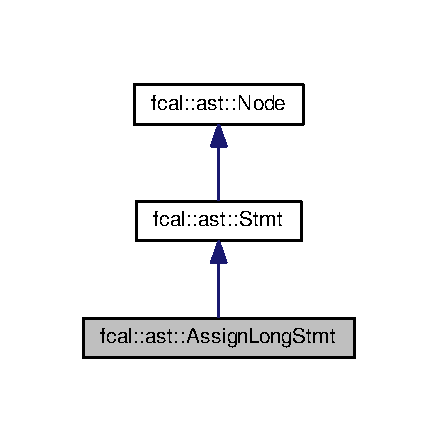
\includegraphics[width=210pt]{classfcal_1_1ast_1_1AssignLongStmt__inherit__graph}
\end{center}
\end{figure}


Collaboration diagram for fcal\+:\+:ast\+:\+:Assign\+Long\+Stmt\+:\nopagebreak
\begin{figure}[H]
\begin{center}
\leavevmode
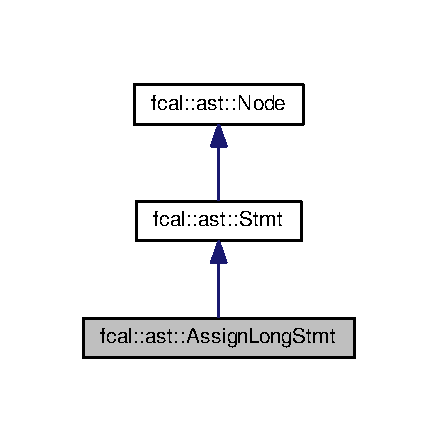
\includegraphics[width=210pt]{classfcal_1_1ast_1_1AssignLongStmt__coll__graph}
\end{center}
\end{figure}
\subsection*{Public Member Functions}
\begin{DoxyCompactItemize}
\item 
\hyperlink{classfcal_1_1ast_1_1AssignLongStmt_a38d5957840878b0dcb69da9da7975a63}{Assign\+Long\+Stmt} (\hyperlink{classfcal_1_1ast_1_1VarName}{Var\+Name} $\ast$var\+\_\+name, \hyperlink{classfcal_1_1ast_1_1Expr}{Expr} $\ast$expr, \hyperlink{classfcal_1_1ast_1_1Expr}{Expr} $\ast$expr2, \hyperlink{classfcal_1_1ast_1_1Expr}{Expr} $\ast$expr3)
\item 
std\+::string \hyperlink{classfcal_1_1ast_1_1AssignLongStmt_a7ff252236eef89c19c8c13c224cf8b81}{unparse} ()
\begin{DoxyCompactList}\small\item\em \hyperlink{classfcal_1_1ast_1_1AssignLongStmt}{Assign\+Long\+Stmt} \hyperlink{classfcal_1_1ast_1_1AssignLongStmt_a7ff252236eef89c19c8c13c224cf8b81}{unparse()} method. \end{DoxyCompactList}\item 
std\+::string {\bfseries cpp\+\_\+code} ()\hypertarget{classfcal_1_1ast_1_1AssignLongStmt_a77fa27de8fddeff175dae275cc3736c5}{}\label{classfcal_1_1ast_1_1AssignLongStmt_a77fa27de8fddeff175dae275cc3736c5}

\end{DoxyCompactItemize}


\subsection{Detailed Description}
The \hyperlink{classfcal_1_1ast_1_1AssignLongStmt}{Assign\+Long\+Stmt} class inherits directly from the abstract \hyperlink{classfcal_1_1ast_1_1Stmt}{Stmt} parent. 

\subsection{Constructor \& Destructor Documentation}
\index{fcal\+::ast\+::\+Assign\+Long\+Stmt@{fcal\+::ast\+::\+Assign\+Long\+Stmt}!Assign\+Long\+Stmt@{Assign\+Long\+Stmt}}
\index{Assign\+Long\+Stmt@{Assign\+Long\+Stmt}!fcal\+::ast\+::\+Assign\+Long\+Stmt@{fcal\+::ast\+::\+Assign\+Long\+Stmt}}
\subsubsection[{\texorpdfstring{Assign\+Long\+Stmt(\+Var\+Name $\ast$var\+\_\+name, Expr $\ast$expr, Expr $\ast$expr2, Expr $\ast$expr3)}{AssignLongStmt(VarName *var_name, Expr *expr, Expr *expr2, Expr *expr3)}}]{\setlength{\rightskip}{0pt plus 5cm}fcal\+::ast\+::\+Assign\+Long\+Stmt\+::\+Assign\+Long\+Stmt (
\begin{DoxyParamCaption}
\item[{{\bf Var\+Name} $\ast$}]{var\+\_\+name, }
\item[{{\bf Expr} $\ast$}]{expr, }
\item[{{\bf Expr} $\ast$}]{expr2, }
\item[{{\bf Expr} $\ast$}]{expr3}
\end{DoxyParamCaption}
)\hspace{0.3cm}{\ttfamily [inline]}, {\ttfamily [explicit]}}\hypertarget{classfcal_1_1ast_1_1AssignLongStmt_a38d5957840878b0dcb69da9da7975a63}{}\label{classfcal_1_1ast_1_1AssignLongStmt_a38d5957840878b0dcb69da9da7975a63}
\hyperlink{classfcal_1_1ast_1_1AssignLongStmt}{Assign\+Long\+Stmt} production class takes the parameters\+: $\ast$var\+\_\+name, $\ast$expr, expr2, and $\ast$expr3 
\begin{DoxyParams}{Parameters}
{\em $\ast$var\+\_\+name} & is the name of the variable being assigned \\
\hline
{\em $\ast$expr} & is the first parameter in a matrix sequence \\
\hline
{\em $\ast$expr2} & is the second parameter in a matrix sequence \\
\hline
{\em $\ast$expr3} & is the expression being assigned to the specific matrix position \\
\hline
\end{DoxyParams}


\subsection{Member Function Documentation}
\index{fcal\+::ast\+::\+Assign\+Long\+Stmt@{fcal\+::ast\+::\+Assign\+Long\+Stmt}!unparse@{unparse}}
\index{unparse@{unparse}!fcal\+::ast\+::\+Assign\+Long\+Stmt@{fcal\+::ast\+::\+Assign\+Long\+Stmt}}
\subsubsection[{\texorpdfstring{unparse()}{unparse()}}]{\setlength{\rightskip}{0pt plus 5cm}std\+::string fcal\+::ast\+::\+Assign\+Long\+Stmt\+::unparse (
\begin{DoxyParamCaption}
{}
\end{DoxyParamCaption}
)\hspace{0.3cm}{\ttfamily [virtual]}}\hypertarget{classfcal_1_1ast_1_1AssignLongStmt_a7ff252236eef89c19c8c13c224cf8b81}{}\label{classfcal_1_1ast_1_1AssignLongStmt_a7ff252236eef89c19c8c13c224cf8b81}


\hyperlink{classfcal_1_1ast_1_1AssignLongStmt}{Assign\+Long\+Stmt} \hyperlink{classfcal_1_1ast_1_1AssignLongStmt_a7ff252236eef89c19c8c13c224cf8b81}{unparse()} method. 

\hyperlink{classfcal_1_1ast_1_1AssignLongStmt}{Assign\+Long\+Stmt} \hyperlink{classfcal_1_1ast_1_1AssignLongStmt_a7ff252236eef89c19c8c13c224cf8b81}{unparse()} returns var\+\_\+name\+\_\+, expr\+\_\+, expr2\+\_\+ and expr3\+\_\+. 

Implements \hyperlink{classfcal_1_1ast_1_1Node_a81865f5a1df593708a39bf492952742a}{fcal\+::ast\+::\+Node}.



The documentation for this class was generated from the following files\+:\begin{DoxyCompactItemize}
\item 
include/ast.\+h\item 
src/ast.\+cc\end{DoxyCompactItemize}

\hypertarget{classfcal_1_1ast_1_1AssignStmt}{}\section{fcal\+:\+:ast\+:\+:Assign\+Stmt Class Reference}
\label{classfcal_1_1ast_1_1AssignStmt}\index{fcal\+::ast\+::\+Assign\+Stmt@{fcal\+::ast\+::\+Assign\+Stmt}}


The \hyperlink{classfcal_1_1ast_1_1AssignStmt}{Assign\+Stmt} class inherits directly from the abstract \hyperlink{classfcal_1_1ast_1_1Stmt}{Stmt} parent class.  




{\ttfamily \#include $<$ast.\+h$>$}



Inheritance diagram for fcal\+:\+:ast\+:\+:Assign\+Stmt\+:\nopagebreak
\begin{figure}[H]
\begin{center}
\leavevmode
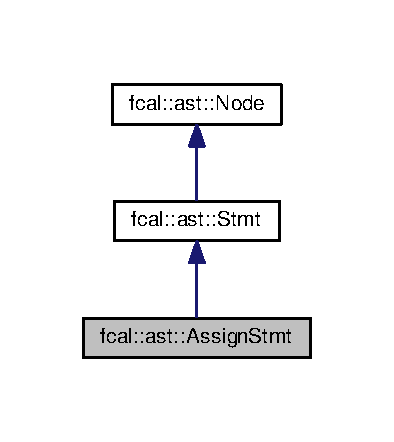
\includegraphics[width=189pt]{classfcal_1_1ast_1_1AssignStmt__inherit__graph}
\end{center}
\end{figure}


Collaboration diagram for fcal\+:\+:ast\+:\+:Assign\+Stmt\+:\nopagebreak
\begin{figure}[H]
\begin{center}
\leavevmode
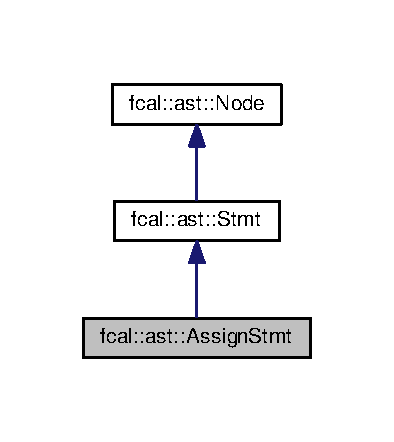
\includegraphics[width=189pt]{classfcal_1_1ast_1_1AssignStmt__coll__graph}
\end{center}
\end{figure}
\subsection*{Public Member Functions}
\begin{DoxyCompactItemize}
\item 
\hyperlink{classfcal_1_1ast_1_1AssignStmt_af73e7e2328c592bf74621873480d063b}{Assign\+Stmt} (\hyperlink{classfcal_1_1ast_1_1VarName}{Var\+Name} $\ast$var\+\_\+name, \hyperlink{classfcal_1_1ast_1_1Expr}{Expr} $\ast$expr)
\item 
std\+::string \hyperlink{classfcal_1_1ast_1_1AssignStmt_ae58f8af8bc26ae0994d95ae266433ded}{unparse} ()
\begin{DoxyCompactList}\small\item\em \hyperlink{classfcal_1_1ast_1_1AssignStmt}{Assign\+Stmt} \hyperlink{classfcal_1_1ast_1_1AssignStmt_ae58f8af8bc26ae0994d95ae266433ded}{unparse()} method. \end{DoxyCompactList}\item 
std\+::string {\bfseries cpp\+\_\+code} ()\hypertarget{classfcal_1_1ast_1_1AssignStmt_a0d6dbae495e452e2d7fc6eb4b5fc41f6}{}\label{classfcal_1_1ast_1_1AssignStmt_a0d6dbae495e452e2d7fc6eb4b5fc41f6}

\end{DoxyCompactItemize}


\subsection{Detailed Description}
The \hyperlink{classfcal_1_1ast_1_1AssignStmt}{Assign\+Stmt} class inherits directly from the abstract \hyperlink{classfcal_1_1ast_1_1Stmt}{Stmt} parent class. 

\subsection{Constructor \& Destructor Documentation}
\index{fcal\+::ast\+::\+Assign\+Stmt@{fcal\+::ast\+::\+Assign\+Stmt}!Assign\+Stmt@{Assign\+Stmt}}
\index{Assign\+Stmt@{Assign\+Stmt}!fcal\+::ast\+::\+Assign\+Stmt@{fcal\+::ast\+::\+Assign\+Stmt}}
\subsubsection[{\texorpdfstring{Assign\+Stmt(\+Var\+Name $\ast$var\+\_\+name, Expr $\ast$expr)}{AssignStmt(VarName *var_name, Expr *expr)}}]{\setlength{\rightskip}{0pt plus 5cm}fcal\+::ast\+::\+Assign\+Stmt\+::\+Assign\+Stmt (
\begin{DoxyParamCaption}
\item[{{\bf Var\+Name} $\ast$}]{var\+\_\+name, }
\item[{{\bf Expr} $\ast$}]{expr}
\end{DoxyParamCaption}
)\hspace{0.3cm}{\ttfamily [inline]}, {\ttfamily [explicit]}}\hypertarget{classfcal_1_1ast_1_1AssignStmt_af73e7e2328c592bf74621873480d063b}{}\label{classfcal_1_1ast_1_1AssignStmt_af73e7e2328c592bf74621873480d063b}
\hyperlink{classfcal_1_1ast_1_1AssignStmt}{Assign\+Stmt} production class takes the parameters\+: $\ast$var\+\_\+name and $\ast$expr 
\begin{DoxyParams}{Parameters}
{\em $\ast$var\+\_\+name} & is the name of the variable being assigned \\
\hline
{\em $\ast$expr} & is the expression being assigned to the variable name \\
\hline
\end{DoxyParams}


\subsection{Member Function Documentation}
\index{fcal\+::ast\+::\+Assign\+Stmt@{fcal\+::ast\+::\+Assign\+Stmt}!unparse@{unparse}}
\index{unparse@{unparse}!fcal\+::ast\+::\+Assign\+Stmt@{fcal\+::ast\+::\+Assign\+Stmt}}
\subsubsection[{\texorpdfstring{unparse()}{unparse()}}]{\setlength{\rightskip}{0pt plus 5cm}std\+::string fcal\+::ast\+::\+Assign\+Stmt\+::unparse (
\begin{DoxyParamCaption}
{}
\end{DoxyParamCaption}
)\hspace{0.3cm}{\ttfamily [virtual]}}\hypertarget{classfcal_1_1ast_1_1AssignStmt_ae58f8af8bc26ae0994d95ae266433ded}{}\label{classfcal_1_1ast_1_1AssignStmt_ae58f8af8bc26ae0994d95ae266433ded}


\hyperlink{classfcal_1_1ast_1_1AssignStmt}{Assign\+Stmt} \hyperlink{classfcal_1_1ast_1_1AssignStmt_ae58f8af8bc26ae0994d95ae266433ded}{unparse()} method. 

\hyperlink{classfcal_1_1ast_1_1AssignStmt}{Assign\+Stmt} \hyperlink{classfcal_1_1ast_1_1AssignStmt_ae58f8af8bc26ae0994d95ae266433ded}{unparse()} returns var\+\_\+name\+\_\+, expr\+\_\+. 

Implements \hyperlink{classfcal_1_1ast_1_1Node_a81865f5a1df593708a39bf492952742a}{fcal\+::ast\+::\+Node}.



The documentation for this class was generated from the following files\+:\begin{DoxyCompactItemize}
\item 
include/ast.\+h\item 
src/ast.\+cc\end{DoxyCompactItemize}

\hypertarget{classfcal_1_1ast_1_1BinaryOp}{}\section{fcal\+:\+:ast\+:\+:Binary\+Op Class Reference}
\label{classfcal_1_1ast_1_1BinaryOp}\index{fcal\+::ast\+::\+Binary\+Op@{fcal\+::ast\+::\+Binary\+Op}}


{\ttfamily \#include $<$ast.\+h$>$}



Inheritance diagram for fcal\+:\+:ast\+:\+:Binary\+Op\+:
\nopagebreak
\begin{figure}[H]
\begin{center}
\leavevmode
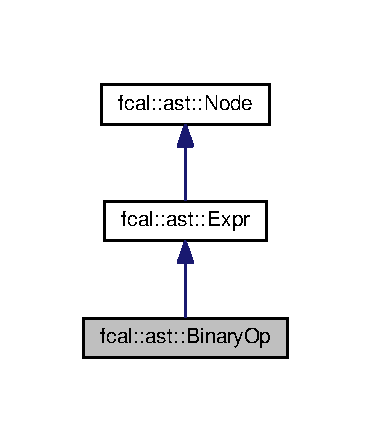
\includegraphics[width=178pt]{classfcal_1_1ast_1_1BinaryOp__inherit__graph}
\end{center}
\end{figure}


Collaboration diagram for fcal\+:\+:ast\+:\+:Binary\+Op\+:
\nopagebreak
\begin{figure}[H]
\begin{center}
\leavevmode
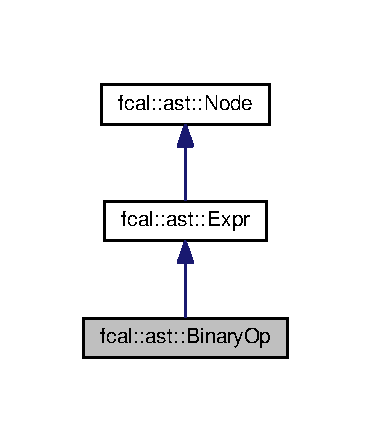
\includegraphics[width=178pt]{classfcal_1_1ast_1_1BinaryOp__coll__graph}
\end{center}
\end{figure}
\subsection*{Public Member Functions}
\begin{DoxyCompactItemize}
\item 
\hyperlink{classfcal_1_1ast_1_1BinaryOp_ad904b6af1e7ac258d9afaa1d6716df51}{Binary\+Op} (\hyperlink{classfcal_1_1ast_1_1Expr}{Expr} $\ast$expr, std\+::string $\ast$op, \hyperlink{classfcal_1_1ast_1_1Expr}{Expr} $\ast$expr2)
\item 
std\+::string \hyperlink{classfcal_1_1ast_1_1BinaryOp_a7f019bd362a138dd80450dfdafd2325a}{unparse} ()
\begin{DoxyCompactList}\small\item\em \hyperlink{classfcal_1_1ast_1_1BinaryOp}{Binary\+Op} \hyperlink{classfcal_1_1ast_1_1BinaryOp_a7f019bd362a138dd80450dfdafd2325a}{unparse()} method. \end{DoxyCompactList}\item 
std\+::string {\bfseries cpp\+\_\+code} ()\hypertarget{classfcal_1_1ast_1_1BinaryOp_a17df80baf8b6fd11dcd827941d6b424f}{}\label{classfcal_1_1ast_1_1BinaryOp_a17df80baf8b6fd11dcd827941d6b424f}

\end{DoxyCompactItemize}


\subsection{Detailed Description}
The \hyperlink{classfcal_1_1ast_1_1BinaryOp}{Binary\+Op} class inherits directly from the parent \hyperlink{classfcal_1_1ast_1_1Expr}{Expr} class. The \hyperlink{classfcal_1_1ast_1_1BinaryOp}{Binary\+Op} class combines the redundant nature of the implementing multiple production rule classes for the various binary operators including\+: $\ast$, /, +, -\/, $>$, $>$=, $<$, $<$=, ==, !=, \&\& and $\vert$$\vert$.

The constructor determines the type of operator associated with expression by defining the $\ast$op to the lexeme of the prev\+\_\+token\+\_\+ for the matched signed. 

\subsection{Constructor \& Destructor Documentation}
\index{fcal\+::ast\+::\+Binary\+Op@{fcal\+::ast\+::\+Binary\+Op}!Binary\+Op@{Binary\+Op}}
\index{Binary\+Op@{Binary\+Op}!fcal\+::ast\+::\+Binary\+Op@{fcal\+::ast\+::\+Binary\+Op}}
\subsubsection[{\texorpdfstring{Binary\+Op(\+Expr $\ast$expr, std\+::string $\ast$op, Expr $\ast$expr2)}{BinaryOp(Expr *expr, std::string *op, Expr *expr2)}}]{\setlength{\rightskip}{0pt plus 5cm}fcal\+::ast\+::\+Binary\+Op\+::\+Binary\+Op (
\begin{DoxyParamCaption}
\item[{{\bf Expr} $\ast$}]{expr, }
\item[{std\+::string $\ast$}]{op, }
\item[{{\bf Expr} $\ast$}]{expr2}
\end{DoxyParamCaption}
)\hspace{0.3cm}{\ttfamily [inline]}, {\ttfamily [explicit]}}\hypertarget{classfcal_1_1ast_1_1BinaryOp_ad904b6af1e7ac258d9afaa1d6716df51}{}\label{classfcal_1_1ast_1_1BinaryOp_ad904b6af1e7ac258d9afaa1d6716df51}
\hyperlink{classfcal_1_1ast_1_1BinaryOp}{Binary\+Op} production rules take the parameters\+: $\ast$expr, $\ast$op and $\ast$expr2 
\begin{DoxyParams}{Parameters}
{\em $\ast$expr} & is the L\+HS expression \\
\hline
{\em $\ast$op} & is the binary operator \\
\hline
{\em $\ast$expr2} & is the R\+HS expression \\
\hline
\end{DoxyParams}


\subsection{Member Function Documentation}
\index{fcal\+::ast\+::\+Binary\+Op@{fcal\+::ast\+::\+Binary\+Op}!unparse@{unparse}}
\index{unparse@{unparse}!fcal\+::ast\+::\+Binary\+Op@{fcal\+::ast\+::\+Binary\+Op}}
\subsubsection[{\texorpdfstring{unparse()}{unparse()}}]{\setlength{\rightskip}{0pt plus 5cm}std\+::string fcal\+::ast\+::\+Binary\+Op\+::unparse (
\begin{DoxyParamCaption}
{}
\end{DoxyParamCaption}
)\hspace{0.3cm}{\ttfamily [virtual]}}\hypertarget{classfcal_1_1ast_1_1BinaryOp_a7f019bd362a138dd80450dfdafd2325a}{}\label{classfcal_1_1ast_1_1BinaryOp_a7f019bd362a138dd80450dfdafd2325a}


\hyperlink{classfcal_1_1ast_1_1BinaryOp}{Binary\+Op} \hyperlink{classfcal_1_1ast_1_1BinaryOp_a7f019bd362a138dd80450dfdafd2325a}{unparse()} method. 

\hyperlink{classfcal_1_1ast_1_1BinaryOp}{Binary\+Op} returns the expr\+\_\+, op\+\_\+ and expr2\+\_\+. 

Implements \hyperlink{classfcal_1_1ast_1_1Node_a81865f5a1df593708a39bf492952742a}{fcal\+::ast\+::\+Node}.



The documentation for this class was generated from the following files\+:\begin{DoxyCompactItemize}
\item 
include/ast.\+h\item 
src/ast.\+cc\end{DoxyCompactItemize}

\hypertarget{classfcal_1_1ast_1_1BlockStmt}{}\section{fcal\+:\+:ast\+:\+:Block\+Stmt Class Reference}
\label{classfcal_1_1ast_1_1BlockStmt}\index{fcal\+::ast\+::\+Block\+Stmt@{fcal\+::ast\+::\+Block\+Stmt}}


The \hyperlink{classfcal_1_1ast_1_1BlockStmt}{Block\+Stmt} class inherits directly from the abstract \hyperlink{classfcal_1_1ast_1_1Stmt}{Stmt} parent class.  




{\ttfamily \#include $<$ast.\+h$>$}



Inheritance diagram for fcal\+:\+:ast\+:\+:Block\+Stmt\+:\nopagebreak
\begin{figure}[H]
\begin{center}
\leavevmode
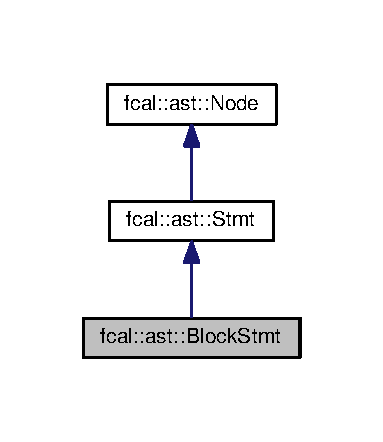
\includegraphics[width=184pt]{classfcal_1_1ast_1_1BlockStmt__inherit__graph}
\end{center}
\end{figure}


Collaboration diagram for fcal\+:\+:ast\+:\+:Block\+Stmt\+:\nopagebreak
\begin{figure}[H]
\begin{center}
\leavevmode
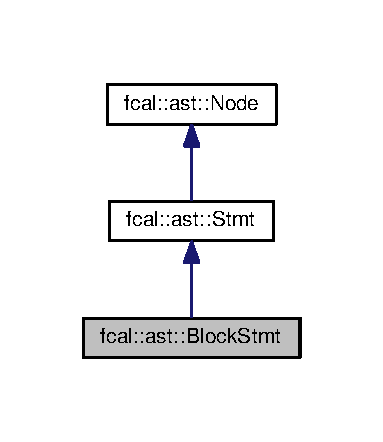
\includegraphics[width=184pt]{classfcal_1_1ast_1_1BlockStmt__coll__graph}
\end{center}
\end{figure}
\subsection*{Public Member Functions}
\begin{DoxyCompactItemize}
\item 
\hyperlink{classfcal_1_1ast_1_1BlockStmt_a066ef99adee82963a793e961ebaacdf1}{Block\+Stmt} (\hyperlink{classfcal_1_1ast_1_1Stmts}{Stmts} $\ast$stmts)
\item 
std\+::string \hyperlink{classfcal_1_1ast_1_1BlockStmt_acecf7901ab8c1a338a5966ad9b7ecb56}{unparse} ()
\begin{DoxyCompactList}\small\item\em \hyperlink{classfcal_1_1ast_1_1BlockStmt}{Block\+Stmt} \hyperlink{classfcal_1_1ast_1_1BlockStmt_acecf7901ab8c1a338a5966ad9b7ecb56}{unparse()} method. \end{DoxyCompactList}\item 
std\+::string {\bfseries cpp\+\_\+code} ()\hypertarget{classfcal_1_1ast_1_1BlockStmt_a8b61f0a6ab8aca5ae7b09a12255f4a17}{}\label{classfcal_1_1ast_1_1BlockStmt_a8b61f0a6ab8aca5ae7b09a12255f4a17}

\end{DoxyCompactItemize}


\subsection{Detailed Description}
The \hyperlink{classfcal_1_1ast_1_1BlockStmt}{Block\+Stmt} class inherits directly from the abstract \hyperlink{classfcal_1_1ast_1_1Stmt}{Stmt} parent class. 

\subsection{Constructor \& Destructor Documentation}
\index{fcal\+::ast\+::\+Block\+Stmt@{fcal\+::ast\+::\+Block\+Stmt}!Block\+Stmt@{Block\+Stmt}}
\index{Block\+Stmt@{Block\+Stmt}!fcal\+::ast\+::\+Block\+Stmt@{fcal\+::ast\+::\+Block\+Stmt}}
\subsubsection[{\texorpdfstring{Block\+Stmt(\+Stmts $\ast$stmts)}{BlockStmt(Stmts *stmts)}}]{\setlength{\rightskip}{0pt plus 5cm}fcal\+::ast\+::\+Block\+Stmt\+::\+Block\+Stmt (
\begin{DoxyParamCaption}
\item[{{\bf Stmts} $\ast$}]{stmts}
\end{DoxyParamCaption}
)\hspace{0.3cm}{\ttfamily [inline]}, {\ttfamily [explicit]}}\hypertarget{classfcal_1_1ast_1_1BlockStmt_a066ef99adee82963a793e961ebaacdf1}{}\label{classfcal_1_1ast_1_1BlockStmt_a066ef99adee82963a793e961ebaacdf1}
\hyperlink{classfcal_1_1ast_1_1BlockStmt}{Block\+Stmt} production class takes a single parameter\+: stmts 
\begin{DoxyParams}{Parameters}
{\em $\ast$stmts} & statements \\
\hline
\end{DoxyParams}


\subsection{Member Function Documentation}
\index{fcal\+::ast\+::\+Block\+Stmt@{fcal\+::ast\+::\+Block\+Stmt}!unparse@{unparse}}
\index{unparse@{unparse}!fcal\+::ast\+::\+Block\+Stmt@{fcal\+::ast\+::\+Block\+Stmt}}
\subsubsection[{\texorpdfstring{unparse()}{unparse()}}]{\setlength{\rightskip}{0pt plus 5cm}std\+::string fcal\+::ast\+::\+Block\+Stmt\+::unparse (
\begin{DoxyParamCaption}
{}
\end{DoxyParamCaption}
)\hspace{0.3cm}{\ttfamily [virtual]}}\hypertarget{classfcal_1_1ast_1_1BlockStmt_acecf7901ab8c1a338a5966ad9b7ecb56}{}\label{classfcal_1_1ast_1_1BlockStmt_acecf7901ab8c1a338a5966ad9b7ecb56}


\hyperlink{classfcal_1_1ast_1_1BlockStmt}{Block\+Stmt} \hyperlink{classfcal_1_1ast_1_1BlockStmt_acecf7901ab8c1a338a5966ad9b7ecb56}{unparse()} method. 

\hyperlink{classfcal_1_1ast_1_1BlockStmt}{Block\+Stmt} \hyperlink{classfcal_1_1ast_1_1BlockStmt_acecf7901ab8c1a338a5966ad9b7ecb56}{unparse()} returns the stmts\+\_\+ parameter. 

Implements \hyperlink{classfcal_1_1ast_1_1Node_a81865f5a1df593708a39bf492952742a}{fcal\+::ast\+::\+Node}.



The documentation for this class was generated from the following files\+:\begin{DoxyCompactItemize}
\item 
include/ast.\+h\item 
src/ast.\+cc\end{DoxyCompactItemize}

\hypertarget{classfcal_1_1ast_1_1BoolFalse}{}\section{fcal\+:\+:ast\+:\+:Bool\+False Class Reference}
\label{classfcal_1_1ast_1_1BoolFalse}\index{fcal\+::ast\+::\+Bool\+False@{fcal\+::ast\+::\+Bool\+False}}


The \hyperlink{classfcal_1_1ast_1_1BoolFalse}{Bool\+False} class inherits directly from the abstract \hyperlink{classfcal_1_1ast_1_1Expr}{Expr} class.  




{\ttfamily \#include $<$ast.\+h$>$}



Inheritance diagram for fcal\+:\+:ast\+:\+:Bool\+False\+:\nopagebreak
\begin{figure}[H]
\begin{center}
\leavevmode
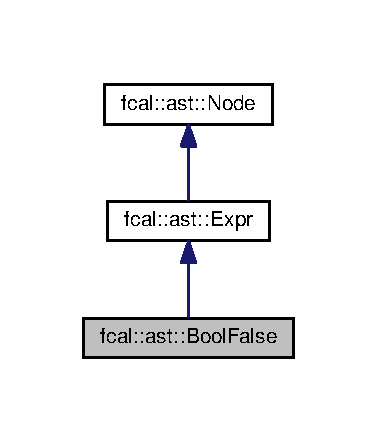
\includegraphics[width=181pt]{classfcal_1_1ast_1_1BoolFalse__inherit__graph}
\end{center}
\end{figure}


Collaboration diagram for fcal\+:\+:ast\+:\+:Bool\+False\+:\nopagebreak
\begin{figure}[H]
\begin{center}
\leavevmode
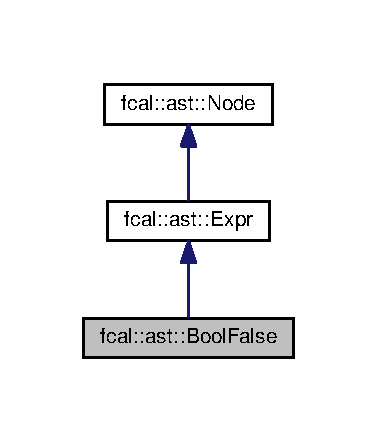
\includegraphics[width=181pt]{classfcal_1_1ast_1_1BoolFalse__coll__graph}
\end{center}
\end{figure}
\subsection*{Public Member Functions}
\begin{DoxyCompactItemize}
\item 
\hyperlink{classfcal_1_1ast_1_1BoolFalse_a38a3fc84a3b5028b659fa79036ecd91c}{Bool\+False} ()\hypertarget{classfcal_1_1ast_1_1BoolFalse_a38a3fc84a3b5028b659fa79036ecd91c}{}\label{classfcal_1_1ast_1_1BoolFalse_a38a3fc84a3b5028b659fa79036ecd91c}

\begin{DoxyCompactList}\small\item\em \hyperlink{classfcal_1_1ast_1_1BoolFalse_a38a3fc84a3b5028b659fa79036ecd91c}{Bool\+False()} constructor. \end{DoxyCompactList}\item 
std\+::string \hyperlink{classfcal_1_1ast_1_1BoolFalse_ae0ed05097f347fb87cdaefd115168f94}{unparse} ()
\begin{DoxyCompactList}\small\item\em \hyperlink{classfcal_1_1ast_1_1BoolFalse}{Bool\+False} \hyperlink{classfcal_1_1ast_1_1BoolFalse_ae0ed05097f347fb87cdaefd115168f94}{unparse()} method. \end{DoxyCompactList}\item 
std\+::string {\bfseries cpp\+\_\+code} ()\hypertarget{classfcal_1_1ast_1_1BoolFalse_a6e2f4bb07915ed96e9e183ffa16578a0}{}\label{classfcal_1_1ast_1_1BoolFalse_a6e2f4bb07915ed96e9e183ffa16578a0}

\end{DoxyCompactItemize}


\subsection{Detailed Description}
The \hyperlink{classfcal_1_1ast_1_1BoolFalse}{Bool\+False} class inherits directly from the abstract \hyperlink{classfcal_1_1ast_1_1Expr}{Expr} class. 

\subsection{Member Function Documentation}
\index{fcal\+::ast\+::\+Bool\+False@{fcal\+::ast\+::\+Bool\+False}!unparse@{unparse}}
\index{unparse@{unparse}!fcal\+::ast\+::\+Bool\+False@{fcal\+::ast\+::\+Bool\+False}}
\subsubsection[{\texorpdfstring{unparse()}{unparse()}}]{\setlength{\rightskip}{0pt plus 5cm}std\+::string fcal\+::ast\+::\+Bool\+False\+::unparse (
\begin{DoxyParamCaption}
{}
\end{DoxyParamCaption}
)\hspace{0.3cm}{\ttfamily [virtual]}}\hypertarget{classfcal_1_1ast_1_1BoolFalse_ae0ed05097f347fb87cdaefd115168f94}{}\label{classfcal_1_1ast_1_1BoolFalse_ae0ed05097f347fb87cdaefd115168f94}


\hyperlink{classfcal_1_1ast_1_1BoolFalse}{Bool\+False} \hyperlink{classfcal_1_1ast_1_1BoolFalse_ae0ed05097f347fb87cdaefd115168f94}{unparse()} method. 

\hyperlink{classfcal_1_1ast_1_1BoolFalse}{Bool\+False} returns a \char`\"{}\+False\char`\"{} string for a boolean false. 

Implements \hyperlink{classfcal_1_1ast_1_1Node_a81865f5a1df593708a39bf492952742a}{fcal\+::ast\+::\+Node}.



The documentation for this class was generated from the following files\+:\begin{DoxyCompactItemize}
\item 
include/ast.\+h\item 
src/ast.\+cc\end{DoxyCompactItemize}

\hypertarget{classfcal_1_1ast_1_1BoolTrue}{}\section{fcal\+:\+:ast\+:\+:Bool\+True Class Reference}
\label{classfcal_1_1ast_1_1BoolTrue}\index{fcal\+::ast\+::\+Bool\+True@{fcal\+::ast\+::\+Bool\+True}}


The \hyperlink{classfcal_1_1ast_1_1BoolTrue}{Bool\+True} class inherits directly from the abstract \hyperlink{classfcal_1_1ast_1_1Expr}{Expr} class.  




{\ttfamily \#include $<$ast.\+h$>$}



Inheritance diagram for fcal\+:\+:ast\+:\+:Bool\+True\+:
\nopagebreak
\begin{figure}[H]
\begin{center}
\leavevmode
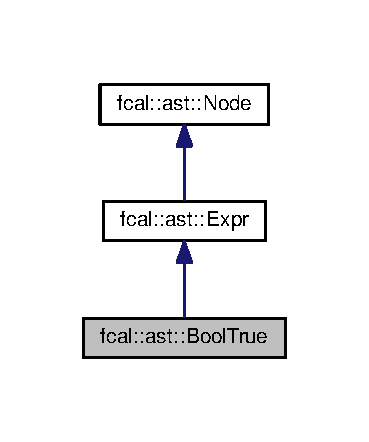
\includegraphics[width=177pt]{classfcal_1_1ast_1_1BoolTrue__inherit__graph}
\end{center}
\end{figure}


Collaboration diagram for fcal\+:\+:ast\+:\+:Bool\+True\+:
\nopagebreak
\begin{figure}[H]
\begin{center}
\leavevmode
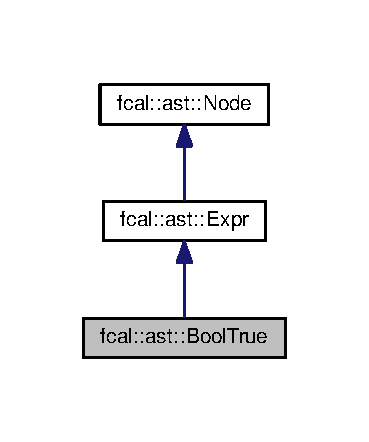
\includegraphics[width=177pt]{classfcal_1_1ast_1_1BoolTrue__coll__graph}
\end{center}
\end{figure}
\subsection*{Public Member Functions}
\begin{DoxyCompactItemize}
\item 
\hyperlink{classfcal_1_1ast_1_1BoolTrue_acc7f964d0dce8fa53de59eea835bb69c}{Bool\+True} ()\hypertarget{classfcal_1_1ast_1_1BoolTrue_acc7f964d0dce8fa53de59eea835bb69c}{}\label{classfcal_1_1ast_1_1BoolTrue_acc7f964d0dce8fa53de59eea835bb69c}

\begin{DoxyCompactList}\small\item\em \hyperlink{classfcal_1_1ast_1_1BoolTrue_acc7f964d0dce8fa53de59eea835bb69c}{Bool\+True()} constructor. \end{DoxyCompactList}\item 
std\+::string \hyperlink{classfcal_1_1ast_1_1BoolTrue_a1467c30c135c099ea80f19f965bddca8}{unparse} ()
\begin{DoxyCompactList}\small\item\em \hyperlink{classfcal_1_1ast_1_1BoolTrue}{Bool\+True} \hyperlink{classfcal_1_1ast_1_1BoolTrue_a1467c30c135c099ea80f19f965bddca8}{unparse()} method. \end{DoxyCompactList}\item 
std\+::string {\bfseries cpp\+\_\+code} ()\hypertarget{classfcal_1_1ast_1_1BoolTrue_a82b6d3221f2d17af809f04b55f75b0e3}{}\label{classfcal_1_1ast_1_1BoolTrue_a82b6d3221f2d17af809f04b55f75b0e3}

\end{DoxyCompactItemize}


\subsection{Detailed Description}
The \hyperlink{classfcal_1_1ast_1_1BoolTrue}{Bool\+True} class inherits directly from the abstract \hyperlink{classfcal_1_1ast_1_1Expr}{Expr} class. 

\subsection{Member Function Documentation}
\index{fcal\+::ast\+::\+Bool\+True@{fcal\+::ast\+::\+Bool\+True}!unparse@{unparse}}
\index{unparse@{unparse}!fcal\+::ast\+::\+Bool\+True@{fcal\+::ast\+::\+Bool\+True}}
\subsubsection[{\texorpdfstring{unparse()}{unparse()}}]{\setlength{\rightskip}{0pt plus 5cm}std\+::string fcal\+::ast\+::\+Bool\+True\+::unparse (
\begin{DoxyParamCaption}
{}
\end{DoxyParamCaption}
)\hspace{0.3cm}{\ttfamily [virtual]}}\hypertarget{classfcal_1_1ast_1_1BoolTrue_a1467c30c135c099ea80f19f965bddca8}{}\label{classfcal_1_1ast_1_1BoolTrue_a1467c30c135c099ea80f19f965bddca8}


\hyperlink{classfcal_1_1ast_1_1BoolTrue}{Bool\+True} \hyperlink{classfcal_1_1ast_1_1BoolTrue_a1467c30c135c099ea80f19f965bddca8}{unparse()} method. 

\hyperlink{classfcal_1_1ast_1_1BoolTrue}{Bool\+True} returns the \char`\"{}\+True\char`\"{} string for a boolean truth. 

Implements \hyperlink{classfcal_1_1ast_1_1Node_a81865f5a1df593708a39bf492952742a}{fcal\+::ast\+::\+Node}.



The documentation for this class was generated from the following files\+:\begin{DoxyCompactItemize}
\item 
include/ast.\+h\item 
src/ast.\+cc\end{DoxyCompactItemize}

\hypertarget{classfcal_1_1scanner_1_1CharConstToken}{}\section{fcal\+:\+:scanner\+:\+:Char\+Const\+Token Class Reference}
\label{classfcal_1_1scanner_1_1CharConstToken}\index{fcal\+::scanner\+::\+Char\+Const\+Token@{fcal\+::scanner\+::\+Char\+Const\+Token}}


Inheritance diagram for fcal\+:\+:scanner\+:\+:Char\+Const\+Token\+:
\nopagebreak
\begin{figure}[H]
\begin{center}
\leavevmode
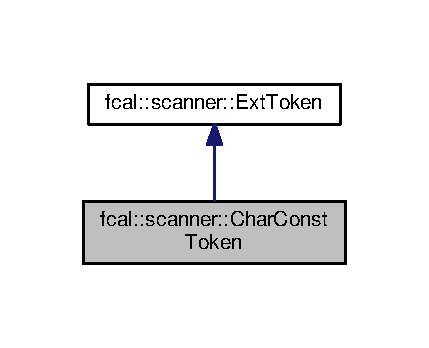
\includegraphics[width=206pt]{classfcal_1_1scanner_1_1CharConstToken__inherit__graph}
\end{center}
\end{figure}


Collaboration diagram for fcal\+:\+:scanner\+:\+:Char\+Const\+Token\+:
\nopagebreak
\begin{figure}[H]
\begin{center}
\leavevmode
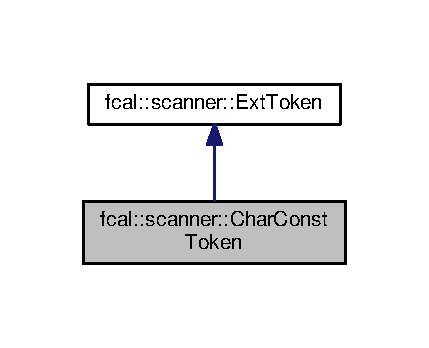
\includegraphics[width=206pt]{classfcal_1_1scanner_1_1CharConstToken__coll__graph}
\end{center}
\end{figure}
\subsection*{Public Member Functions}
\begin{DoxyCompactItemize}
\item 
{\bfseries Char\+Const\+Token} (\hyperlink{classfcal_1_1parser_1_1Parser}{parser\+::\+Parser} $\ast$p, \hyperlink{classfcal_1_1scanner_1_1Token}{Token} $\ast$t)\hypertarget{classfcal_1_1scanner_1_1CharConstToken_ae108041381482344ee7cf3bf0629fbba}{}\label{classfcal_1_1scanner_1_1CharConstToken_ae108041381482344ee7cf3bf0629fbba}

\item 
\hyperlink{classfcal_1_1parser_1_1ParseResult}{parser\+::\+Parse\+Result} {\bfseries nud} ()\hypertarget{classfcal_1_1scanner_1_1CharConstToken_a5e9299e684f969cde0f71c0041e92153}{}\label{classfcal_1_1scanner_1_1CharConstToken_a5e9299e684f969cde0f71c0041e92153}

\item 
std\+::string {\bfseries description} ()\hypertarget{classfcal_1_1scanner_1_1CharConstToken_a283d5fb12d36caac1afed73c1035b562}{}\label{classfcal_1_1scanner_1_1CharConstToken_a283d5fb12d36caac1afed73c1035b562}

\end{DoxyCompactItemize}
\subsection*{Additional Inherited Members}


The documentation for this class was generated from the following file\+:\begin{DoxyCompactItemize}
\item 
include/ext\+\_\+token.\+h\end{DoxyCompactItemize}

\hypertarget{classfcal_1_1scanner_1_1DashToken}{}\section{fcal\+:\+:scanner\+:\+:Dash\+Token Class Reference}
\label{classfcal_1_1scanner_1_1DashToken}\index{fcal\+::scanner\+::\+Dash\+Token@{fcal\+::scanner\+::\+Dash\+Token}}


Inheritance diagram for fcal\+:\+:scanner\+:\+:Dash\+Token\+:
\nopagebreak
\begin{figure}[H]
\begin{center}
\leavevmode
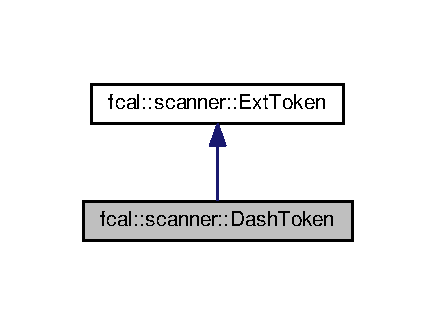
\includegraphics[width=209pt]{classfcal_1_1scanner_1_1DashToken__inherit__graph}
\end{center}
\end{figure}


Collaboration diagram for fcal\+:\+:scanner\+:\+:Dash\+Token\+:
\nopagebreak
\begin{figure}[H]
\begin{center}
\leavevmode
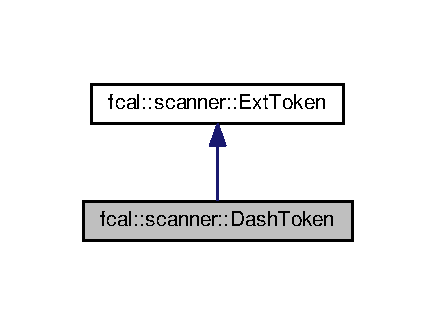
\includegraphics[width=209pt]{classfcal_1_1scanner_1_1DashToken__coll__graph}
\end{center}
\end{figure}
\subsection*{Public Member Functions}
\begin{DoxyCompactItemize}
\item 
{\bfseries Dash\+Token} (\hyperlink{classfcal_1_1parser_1_1Parser}{parser\+::\+Parser} $\ast$p, \hyperlink{classfcal_1_1scanner_1_1Token}{Token} $\ast$t)\hypertarget{classfcal_1_1scanner_1_1DashToken_afaabbf1a78e35a4592cd8a5e1bfab79f}{}\label{classfcal_1_1scanner_1_1DashToken_afaabbf1a78e35a4592cd8a5e1bfab79f}

\item 
\hyperlink{classfcal_1_1parser_1_1ParseResult}{parser\+::\+Parse\+Result} {\bfseries led} (\hyperlink{classfcal_1_1parser_1_1ParseResult}{parser\+::\+Parse\+Result} left)\hypertarget{classfcal_1_1scanner_1_1DashToken_a7c0e98c83937cf698ce6f32380e17c52}{}\label{classfcal_1_1scanner_1_1DashToken_a7c0e98c83937cf698ce6f32380e17c52}

\item 
std\+::string {\bfseries description} ()\hypertarget{classfcal_1_1scanner_1_1DashToken_a87476e28739d1c9966ed330ba8154342}{}\label{classfcal_1_1scanner_1_1DashToken_a87476e28739d1c9966ed330ba8154342}

\item 
int {\bfseries lbp} ()\hypertarget{classfcal_1_1scanner_1_1DashToken_a1b88432765ae6c30be1250015ebaa2c4}{}\label{classfcal_1_1scanner_1_1DashToken_a1b88432765ae6c30be1250015ebaa2c4}

\end{DoxyCompactItemize}
\subsection*{Additional Inherited Members}


The documentation for this class was generated from the following file\+:\begin{DoxyCompactItemize}
\item 
include/ext\+\_\+token.\+h\end{DoxyCompactItemize}

\hypertarget{classfcal_1_1ast_1_1Decl}{}\section{fcal\+:\+:ast\+:\+:Decl Class Reference}
\label{classfcal_1_1ast_1_1Decl}\index{fcal\+::ast\+::\+Decl@{fcal\+::ast\+::\+Decl}}


{\ttfamily \#include $<$ast.\+h$>$}



Inheritance diagram for fcal\+:\+:ast\+:\+:Decl\+:
\nopagebreak
\begin{figure}[H]
\begin{center}
\leavevmode
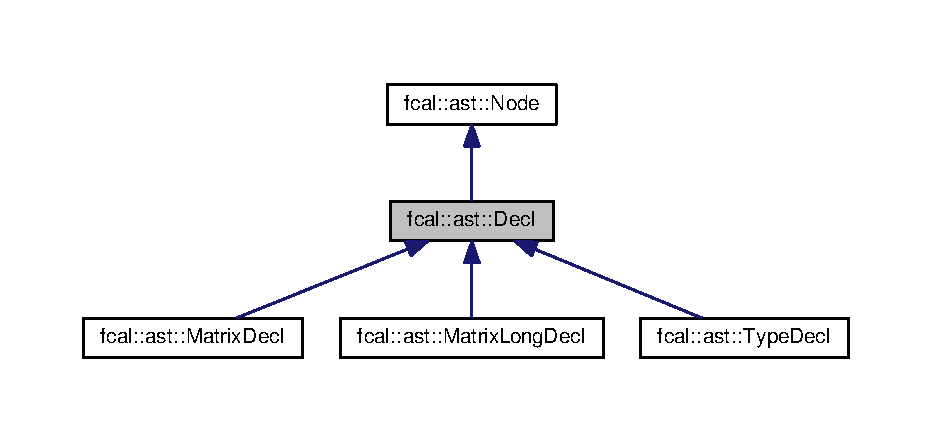
\includegraphics[width=350pt]{classfcal_1_1ast_1_1Decl__inherit__graph}
\end{center}
\end{figure}


Collaboration diagram for fcal\+:\+:ast\+:\+:Decl\+:
\nopagebreak
\begin{figure}[H]
\begin{center}
\leavevmode
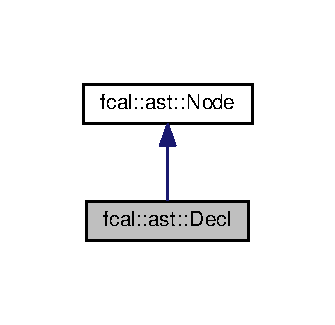
\includegraphics[width=161pt]{classfcal_1_1ast_1_1Decl__coll__graph}
\end{center}
\end{figure}
\subsection*{Additional Inherited Members}


\subsection{Detailed Description}
This is an abstract \hyperlink{classfcal_1_1ast_1_1Decl}{Decl} class that inherits directly from the parent \hyperlink{classfcal_1_1ast_1_1Node}{Node} class. 

The documentation for this class was generated from the following file\+:\begin{DoxyCompactItemize}
\item 
include/ast.\+h\end{DoxyCompactItemize}

\hypertarget{classfcal_1_1ast_1_1EmptyStmts}{}\section{fcal\+:\+:ast\+:\+:Empty\+Stmts Class Reference}
\label{classfcal_1_1ast_1_1EmptyStmts}\index{fcal\+::ast\+::\+Empty\+Stmts@{fcal\+::ast\+::\+Empty\+Stmts}}


The \hyperlink{classfcal_1_1ast_1_1EmptyStmts}{Empty\+Stmts} class inherits directly from the abstract \hyperlink{classfcal_1_1ast_1_1Stmts}{Stmts} parent class.  




{\ttfamily \#include $<$ast.\+h$>$}



Inheritance diagram for fcal\+:\+:ast\+:\+:Empty\+Stmts\+:
\nopagebreak
\begin{figure}[H]
\begin{center}
\leavevmode
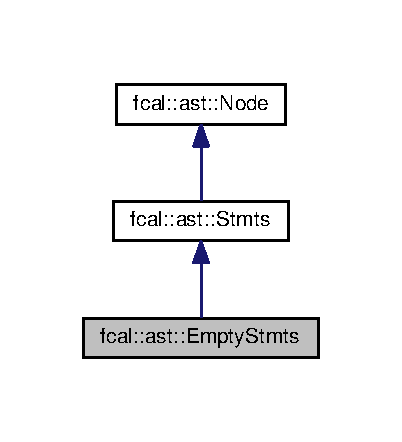
\includegraphics[width=193pt]{classfcal_1_1ast_1_1EmptyStmts__inherit__graph}
\end{center}
\end{figure}


Collaboration diagram for fcal\+:\+:ast\+:\+:Empty\+Stmts\+:
\nopagebreak
\begin{figure}[H]
\begin{center}
\leavevmode
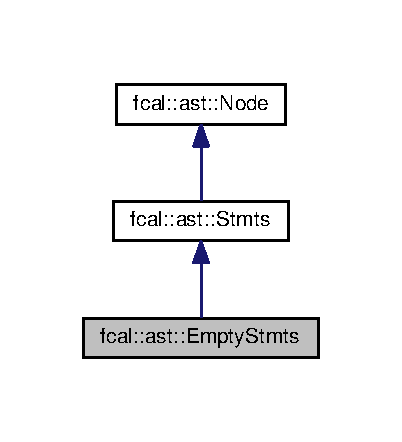
\includegraphics[width=193pt]{classfcal_1_1ast_1_1EmptyStmts__coll__graph}
\end{center}
\end{figure}
\subsection*{Public Member Functions}
\begin{DoxyCompactItemize}
\item 
\hyperlink{classfcal_1_1ast_1_1EmptyStmts_a3fffb31d194ba39a3f7cb22a75dba005}{Empty\+Stmts} ()\hypertarget{classfcal_1_1ast_1_1EmptyStmts_a3fffb31d194ba39a3f7cb22a75dba005}{}\label{classfcal_1_1ast_1_1EmptyStmts_a3fffb31d194ba39a3f7cb22a75dba005}

\begin{DoxyCompactList}\small\item\em \hyperlink{classfcal_1_1ast_1_1EmptyStmts}{Empty\+Stmts} Deconstructor. \end{DoxyCompactList}\item 
std\+::string \hyperlink{classfcal_1_1ast_1_1EmptyStmts_abbccd9fb3e02082962774479fc47116d}{unparse} ()
\begin{DoxyCompactList}\small\item\em \hyperlink{classfcal_1_1ast_1_1EmptyStmts}{Empty\+Stmts} \hyperlink{classfcal_1_1ast_1_1EmptyStmts_abbccd9fb3e02082962774479fc47116d}{unparse()} method. \end{DoxyCompactList}\item 
std\+::string {\bfseries cpp\+\_\+code} ()\hypertarget{classfcal_1_1ast_1_1EmptyStmts_afeac719b025e227f68dc595dd9c135bd}{}\label{classfcal_1_1ast_1_1EmptyStmts_afeac719b025e227f68dc595dd9c135bd}

\end{DoxyCompactItemize}


\subsection{Detailed Description}
The \hyperlink{classfcal_1_1ast_1_1EmptyStmts}{Empty\+Stmts} class inherits directly from the abstract \hyperlink{classfcal_1_1ast_1_1Stmts}{Stmts} parent class. 

\subsection{Member Function Documentation}
\index{fcal\+::ast\+::\+Empty\+Stmts@{fcal\+::ast\+::\+Empty\+Stmts}!unparse@{unparse}}
\index{unparse@{unparse}!fcal\+::ast\+::\+Empty\+Stmts@{fcal\+::ast\+::\+Empty\+Stmts}}
\subsubsection[{\texorpdfstring{unparse()}{unparse()}}]{\setlength{\rightskip}{0pt plus 5cm}std\+::string fcal\+::ast\+::\+Empty\+Stmts\+::unparse (
\begin{DoxyParamCaption}
{}
\end{DoxyParamCaption}
)\hspace{0.3cm}{\ttfamily [virtual]}}\hypertarget{classfcal_1_1ast_1_1EmptyStmts_abbccd9fb3e02082962774479fc47116d}{}\label{classfcal_1_1ast_1_1EmptyStmts_abbccd9fb3e02082962774479fc47116d}


\hyperlink{classfcal_1_1ast_1_1EmptyStmts}{Empty\+Stmts} \hyperlink{classfcal_1_1ast_1_1EmptyStmts_abbccd9fb3e02082962774479fc47116d}{unparse()} method. 

\hyperlink{classfcal_1_1ast_1_1EmptyStmts}{Empty\+Stmts} \hyperlink{classfcal_1_1ast_1_1EmptyStmts_abbccd9fb3e02082962774479fc47116d}{unparse()} returns nothing. 

Implements \hyperlink{classfcal_1_1ast_1_1Node_a81865f5a1df593708a39bf492952742a}{fcal\+::ast\+::\+Node}.



The documentation for this class was generated from the following files\+:\begin{DoxyCompactItemize}
\item 
include/ast.\+h\item 
src/ast.\+cc\end{DoxyCompactItemize}

\hypertarget{classfcal_1_1scanner_1_1EndOfFileToken}{}\section{fcal\+:\+:scanner\+:\+:End\+Of\+File\+Token Class Reference}
\label{classfcal_1_1scanner_1_1EndOfFileToken}\index{fcal\+::scanner\+::\+End\+Of\+File\+Token@{fcal\+::scanner\+::\+End\+Of\+File\+Token}}


Inheritance diagram for fcal\+:\+:scanner\+:\+:End\+Of\+File\+Token\+:\nopagebreak
\begin{figure}[H]
\begin{center}
\leavevmode
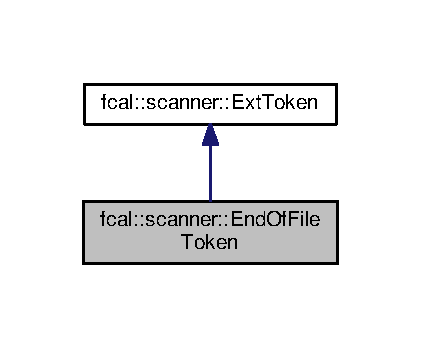
\includegraphics[width=202pt]{classfcal_1_1scanner_1_1EndOfFileToken__inherit__graph}
\end{center}
\end{figure}


Collaboration diagram for fcal\+:\+:scanner\+:\+:End\+Of\+File\+Token\+:\nopagebreak
\begin{figure}[H]
\begin{center}
\leavevmode
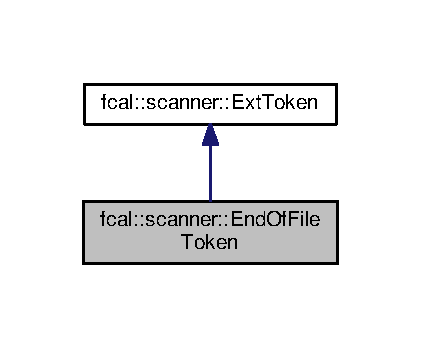
\includegraphics[width=202pt]{classfcal_1_1scanner_1_1EndOfFileToken__coll__graph}
\end{center}
\end{figure}
\subsection*{Public Member Functions}
\begin{DoxyCompactItemize}
\item 
{\bfseries End\+Of\+File\+Token} (\hyperlink{classfcal_1_1parser_1_1Parser}{parser\+::\+Parser} $\ast$p, \hyperlink{classfcal_1_1scanner_1_1Token}{Token} $\ast$t)\hypertarget{classfcal_1_1scanner_1_1EndOfFileToken_a275106595ca3f5a46c80efb281021f2b}{}\label{classfcal_1_1scanner_1_1EndOfFileToken_a275106595ca3f5a46c80efb281021f2b}

\item 
std\+::string {\bfseries description} ()\hypertarget{classfcal_1_1scanner_1_1EndOfFileToken_a8fdfe21df812622405e5b7814970f367}{}\label{classfcal_1_1scanner_1_1EndOfFileToken_a8fdfe21df812622405e5b7814970f367}

\end{DoxyCompactItemize}
\subsection*{Additional Inherited Members}


The documentation for this class was generated from the following file\+:\begin{DoxyCompactItemize}
\item 
include/ext\+\_\+token.\+h\end{DoxyCompactItemize}

\hypertarget{classfcal_1_1ast_1_1EndStmt}{}\section{fcal\+:\+:ast\+:\+:End\+Stmt Class Reference}
\label{classfcal_1_1ast_1_1EndStmt}\index{fcal\+::ast\+::\+End\+Stmt@{fcal\+::ast\+::\+End\+Stmt}}


The \hyperlink{classfcal_1_1ast_1_1EndStmt}{End\+Stmt} class inherits directly from the abstract \hyperlink{classfcal_1_1ast_1_1Stmt}{Stmt} parent class.  




{\ttfamily \#include $<$ast.\+h$>$}



Inheritance diagram for fcal\+:\+:ast\+:\+:End\+Stmt\+:\nopagebreak
\begin{figure}[H]
\begin{center}
\leavevmode
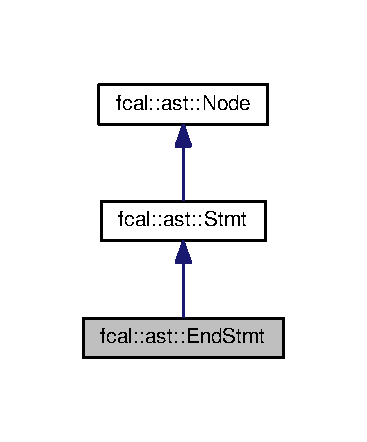
\includegraphics[width=176pt]{classfcal_1_1ast_1_1EndStmt__inherit__graph}
\end{center}
\end{figure}


Collaboration diagram for fcal\+:\+:ast\+:\+:End\+Stmt\+:\nopagebreak
\begin{figure}[H]
\begin{center}
\leavevmode
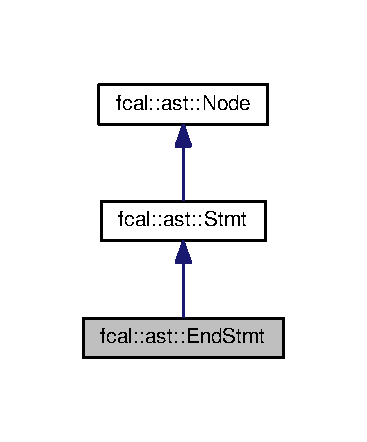
\includegraphics[width=176pt]{classfcal_1_1ast_1_1EndStmt__coll__graph}
\end{center}
\end{figure}
\subsection*{Public Member Functions}
\begin{DoxyCompactItemize}
\item 
\hyperlink{classfcal_1_1ast_1_1EndStmt_afcfe9d73ce8101b449533b389bd21326}{End\+Stmt} ()\hypertarget{classfcal_1_1ast_1_1EndStmt_afcfe9d73ce8101b449533b389bd21326}{}\label{classfcal_1_1ast_1_1EndStmt_afcfe9d73ce8101b449533b389bd21326}

\begin{DoxyCompactList}\small\item\em \hyperlink{classfcal_1_1ast_1_1EndStmt_afcfe9d73ce8101b449533b389bd21326}{End\+Stmt()} constructor. \end{DoxyCompactList}\item 
std\+::string \hyperlink{classfcal_1_1ast_1_1EndStmt_ab1900c9948ccc1a1cd8eca29cebb9baa}{unparse} ()
\begin{DoxyCompactList}\small\item\em \hyperlink{classfcal_1_1ast_1_1EndStmt}{End\+Stmt} \hyperlink{classfcal_1_1ast_1_1EndStmt_ab1900c9948ccc1a1cd8eca29cebb9baa}{unparse()} method. \end{DoxyCompactList}\item 
std\+::string {\bfseries cpp\+\_\+code} ()\hypertarget{classfcal_1_1ast_1_1EndStmt_a1c2355e6142907cf7d42d7cfbca3ec1c}{}\label{classfcal_1_1ast_1_1EndStmt_a1c2355e6142907cf7d42d7cfbca3ec1c}

\end{DoxyCompactItemize}


\subsection{Detailed Description}
The \hyperlink{classfcal_1_1ast_1_1EndStmt}{End\+Stmt} class inherits directly from the abstract \hyperlink{classfcal_1_1ast_1_1Stmt}{Stmt} parent class. 

\subsection{Member Function Documentation}
\index{fcal\+::ast\+::\+End\+Stmt@{fcal\+::ast\+::\+End\+Stmt}!unparse@{unparse}}
\index{unparse@{unparse}!fcal\+::ast\+::\+End\+Stmt@{fcal\+::ast\+::\+End\+Stmt}}
\subsubsection[{\texorpdfstring{unparse()}{unparse()}}]{\setlength{\rightskip}{0pt plus 5cm}std\+::string fcal\+::ast\+::\+End\+Stmt\+::unparse (
\begin{DoxyParamCaption}
{}
\end{DoxyParamCaption}
)\hspace{0.3cm}{\ttfamily [virtual]}}\hypertarget{classfcal_1_1ast_1_1EndStmt_ab1900c9948ccc1a1cd8eca29cebb9baa}{}\label{classfcal_1_1ast_1_1EndStmt_ab1900c9948ccc1a1cd8eca29cebb9baa}


\hyperlink{classfcal_1_1ast_1_1EndStmt}{End\+Stmt} \hyperlink{classfcal_1_1ast_1_1EndStmt_ab1900c9948ccc1a1cd8eca29cebb9baa}{unparse()} method. 

\hyperlink{classfcal_1_1ast_1_1EndStmt}{End\+Stmt} returns a semicolon (;) for end of line. 

Implements \hyperlink{classfcal_1_1ast_1_1Node_a81865f5a1df593708a39bf492952742a}{fcal\+::ast\+::\+Node}.



The documentation for this class was generated from the following files\+:\begin{DoxyCompactItemize}
\item 
include/ast.\+h\item 
src/ast.\+cc\end{DoxyCompactItemize}

\hypertarget{classfcal_1_1ast_1_1Expr}{}\section{fcal\+:\+:ast\+:\+:Expr Class Reference}
\label{classfcal_1_1ast_1_1Expr}\index{fcal\+::ast\+::\+Expr@{fcal\+::ast\+::\+Expr}}


{\ttfamily \#include $<$ast.\+h$>$}



Inheritance diagram for fcal\+:\+:ast\+:\+:Expr\+:
\nopagebreak
\begin{figure}[H]
\begin{center}
\leavevmode
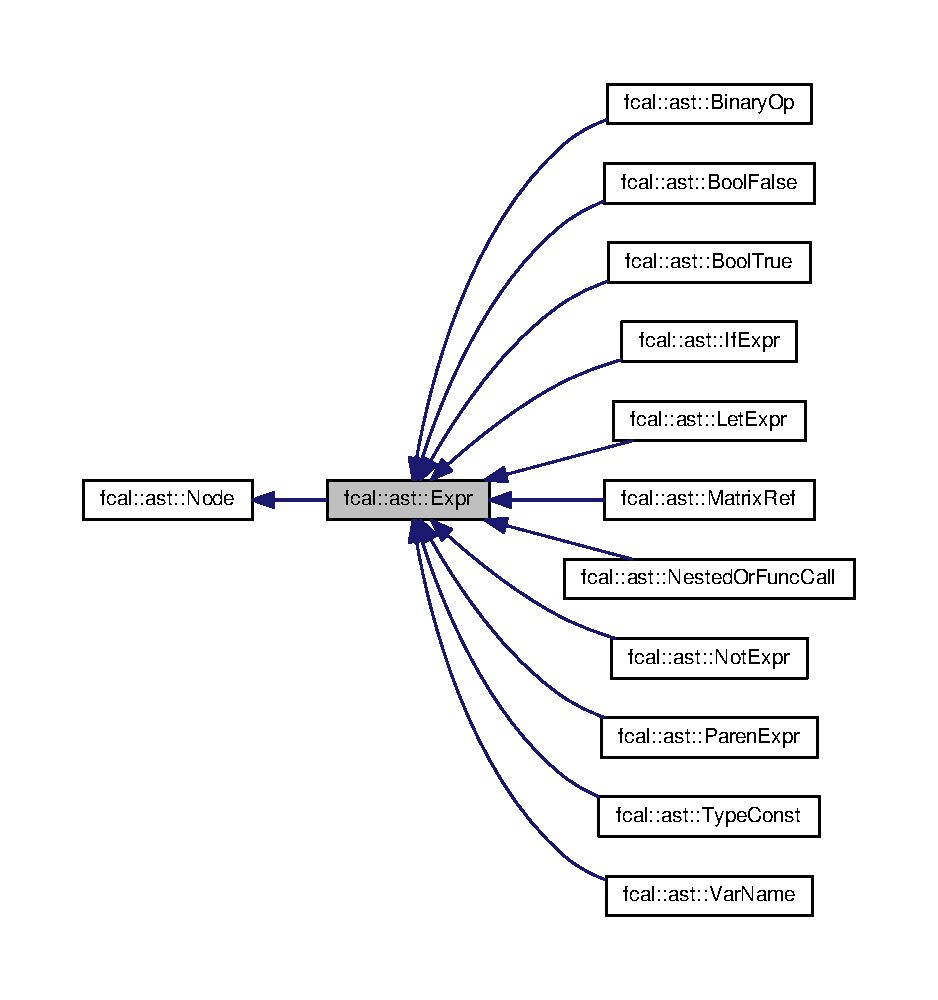
\includegraphics[width=350pt]{classfcal_1_1ast_1_1Expr__inherit__graph}
\end{center}
\end{figure}


Collaboration diagram for fcal\+:\+:ast\+:\+:Expr\+:
\nopagebreak
\begin{figure}[H]
\begin{center}
\leavevmode
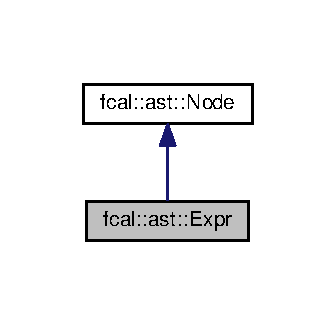
\includegraphics[width=161pt]{classfcal_1_1ast_1_1Expr__coll__graph}
\end{center}
\end{figure}
\subsection*{Additional Inherited Members}


\subsection{Detailed Description}
This is an abstract \hyperlink{classfcal_1_1ast_1_1Expr}{Expr} class that inherits directly from the parent \hyperlink{classfcal_1_1ast_1_1Node}{Node} class. 

The documentation for this class was generated from the following file\+:\begin{DoxyCompactItemize}
\item 
include/ast.\+h\end{DoxyCompactItemize}

\hypertarget{classfcal_1_1scanner_1_1ExtToken}{}\section{fcal\+:\+:scanner\+:\+:Ext\+Token Class Reference}
\label{classfcal_1_1scanner_1_1ExtToken}\index{fcal\+::scanner\+::\+Ext\+Token@{fcal\+::scanner\+::\+Ext\+Token}}


Inheritance diagram for fcal\+:\+:scanner\+:\+:Ext\+Token\+:
\nopagebreak
\begin{figure}[H]
\begin{center}
\leavevmode
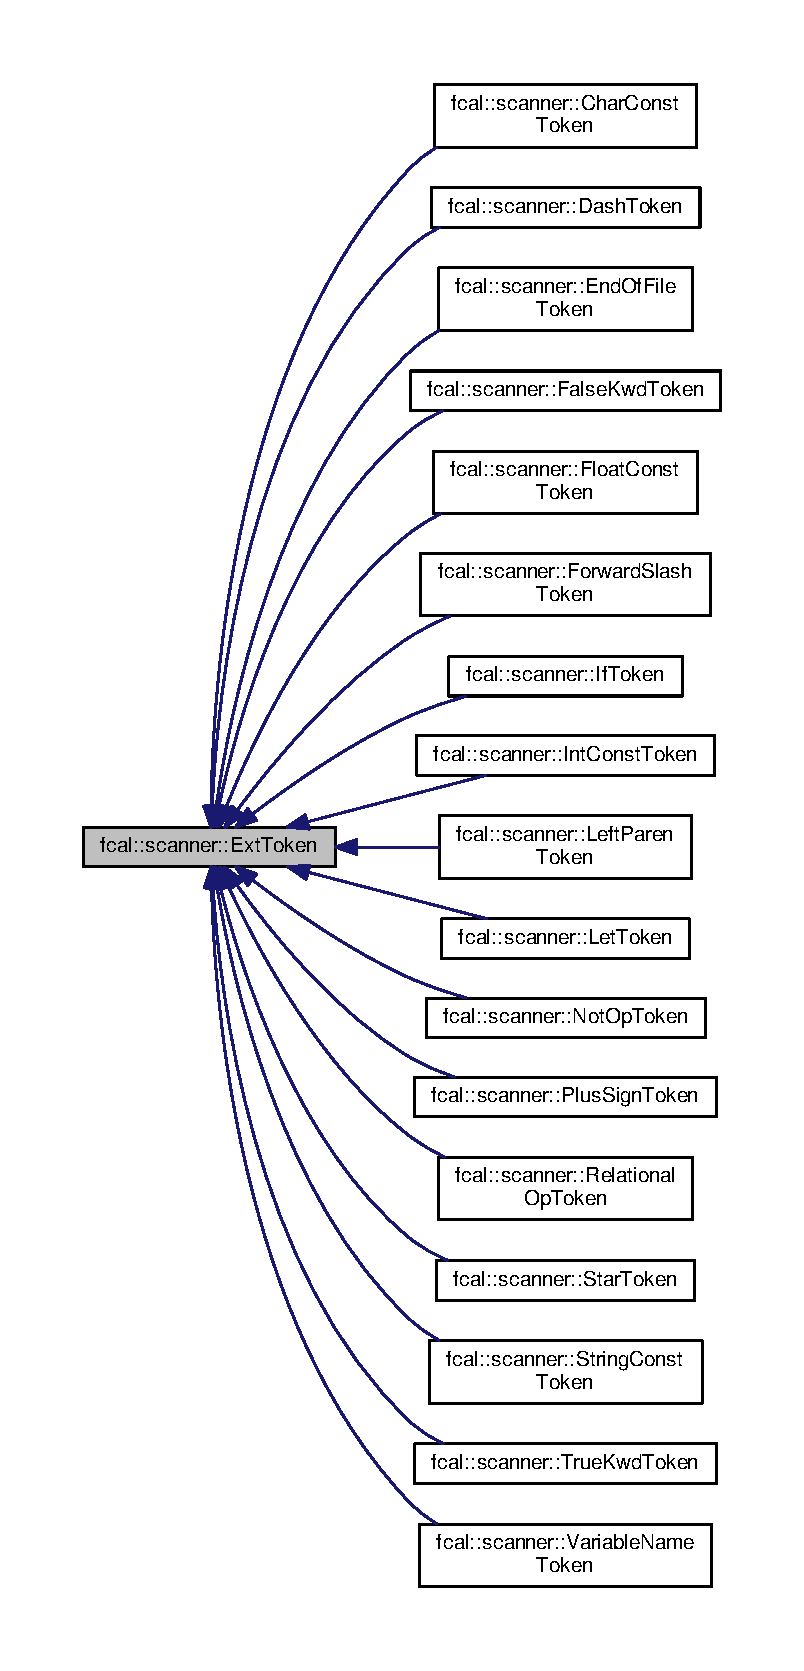
\includegraphics[height=550pt]{classfcal_1_1scanner_1_1ExtToken__inherit__graph}
\end{center}
\end{figure}
\subsection*{Public Member Functions}
\begin{DoxyCompactItemize}
\item 
{\bfseries Ext\+Token} (\hyperlink{classfcal_1_1parser_1_1Parser}{parser\+::\+Parser} $\ast$p, \hyperlink{classfcal_1_1scanner_1_1Token}{Token} $\ast$t)\hypertarget{classfcal_1_1scanner_1_1ExtToken_afda92e9d2c7b66f2b9aaed8ac07bca46}{}\label{classfcal_1_1scanner_1_1ExtToken_afda92e9d2c7b66f2b9aaed8ac07bca46}

\item 
{\bfseries Ext\+Token} (\hyperlink{classfcal_1_1parser_1_1Parser}{parser\+::\+Parser} $\ast$p, \hyperlink{classfcal_1_1scanner_1_1Token}{Token} $\ast$t, std\+::string d)\hypertarget{classfcal_1_1scanner_1_1ExtToken_aa6846c2c9fb91a37715b0f41a0ffcda4}{}\label{classfcal_1_1scanner_1_1ExtToken_aa6846c2c9fb91a37715b0f41a0ffcda4}

\item 
virtual \hyperlink{classfcal_1_1parser_1_1ParseResult}{parser\+::\+Parse\+Result} {\bfseries nud} (void)\hypertarget{classfcal_1_1scanner_1_1ExtToken_a2e1ca27a07d55593ffd67780dbcad7dd}{}\label{classfcal_1_1scanner_1_1ExtToken_a2e1ca27a07d55593ffd67780dbcad7dd}

\item 
virtual \hyperlink{classfcal_1_1parser_1_1ParseResult}{parser\+::\+Parse\+Result} {\bfseries led} (\hyperlink{classfcal_1_1parser_1_1ParseResult}{parser\+::\+Parse\+Result} left)\hypertarget{classfcal_1_1scanner_1_1ExtToken_a42c352ef5e019a1155be80b4a40deb38}{}\label{classfcal_1_1scanner_1_1ExtToken_a42c352ef5e019a1155be80b4a40deb38}

\item 
\hyperlink{classfcal_1_1scanner_1_1ExtToken}{Ext\+Token} $\ast$ {\bfseries Extend\+Token} (\hyperlink{classfcal_1_1parser_1_1Parser}{parser\+::\+Parser} $\ast$p, \hyperlink{classfcal_1_1scanner_1_1Token}{Token} $\ast$tokens)\hypertarget{classfcal_1_1scanner_1_1ExtToken_ad6a5965961553c85d7fbaa688fabf052}{}\label{classfcal_1_1scanner_1_1ExtToken_ad6a5965961553c85d7fbaa688fabf052}

\item 
\hyperlink{classfcal_1_1scanner_1_1ExtToken}{Ext\+Token} $\ast$ {\bfseries Extend\+Token\+List} (\hyperlink{classfcal_1_1parser_1_1Parser}{parser\+::\+Parser} $\ast$p, \hyperlink{classfcal_1_1scanner_1_1Token}{Token} $\ast$tokens)\hypertarget{classfcal_1_1scanner_1_1ExtToken_a4995af1527ea8ba6ee99f3fa8646856d}{}\label{classfcal_1_1scanner_1_1ExtToken_a4995af1527ea8ba6ee99f3fa8646856d}

\item 
virtual int {\bfseries lbp} ()\hypertarget{classfcal_1_1scanner_1_1ExtToken_adecef3770f08e5a26f103ab62171cc91}{}\label{classfcal_1_1scanner_1_1ExtToken_adecef3770f08e5a26f103ab62171cc91}

\item 
virtual std\+::string {\bfseries description} ()\hypertarget{classfcal_1_1scanner_1_1ExtToken_a29a72149492d7fef7968a1b894d334c7}{}\label{classfcal_1_1scanner_1_1ExtToken_a29a72149492d7fef7968a1b894d334c7}

\item 
std\+::string {\bfseries lexeme} (void) const \hypertarget{classfcal_1_1scanner_1_1ExtToken_a32d06bece581a1711625c3a503db21e1}{}\label{classfcal_1_1scanner_1_1ExtToken_a32d06bece581a1711625c3a503db21e1}

\item 
\hyperlink{classfcal_1_1scanner_1_1ExtToken}{Ext\+Token} $\ast$ {\bfseries next} (void) const \hypertarget{classfcal_1_1scanner_1_1ExtToken_aa927cdbdee70b7e74e0aee075f340472}{}\label{classfcal_1_1scanner_1_1ExtToken_aa927cdbdee70b7e74e0aee075f340472}

\item 
scanner\+::\+Token\+Type {\bfseries terminal} (void) const \hypertarget{classfcal_1_1scanner_1_1ExtToken_a0bc057f41ebfeab0900a467af3798bbf}{}\label{classfcal_1_1scanner_1_1ExtToken_a0bc057f41ebfeab0900a467af3798bbf}

\end{DoxyCompactItemize}
\subsection*{Protected Member Functions}
\begin{DoxyCompactItemize}
\item 
\hyperlink{classfcal_1_1parser_1_1Parser}{parser\+::\+Parser} $\ast$ {\bfseries parser} (void)\hypertarget{classfcal_1_1scanner_1_1ExtToken_a311bc29b9732fc7825012ecf08d1d73f}{}\label{classfcal_1_1scanner_1_1ExtToken_a311bc29b9732fc7825012ecf08d1d73f}

\end{DoxyCompactItemize}


The documentation for this class was generated from the following files\+:\begin{DoxyCompactItemize}
\item 
include/ext\+\_\+token.\+h\item 
src/ext\+\_\+token.\+cc\end{DoxyCompactItemize}

\hypertarget{classfcal_1_1scanner_1_1FalseKwdToken}{}\section{fcal\+:\+:scanner\+:\+:False\+Kwd\+Token Class Reference}
\label{classfcal_1_1scanner_1_1FalseKwdToken}\index{fcal\+::scanner\+::\+False\+Kwd\+Token@{fcal\+::scanner\+::\+False\+Kwd\+Token}}


Inheritance diagram for fcal\+:\+:scanner\+:\+:False\+Kwd\+Token\+:\nopagebreak
\begin{figure}[H]
\begin{center}
\leavevmode
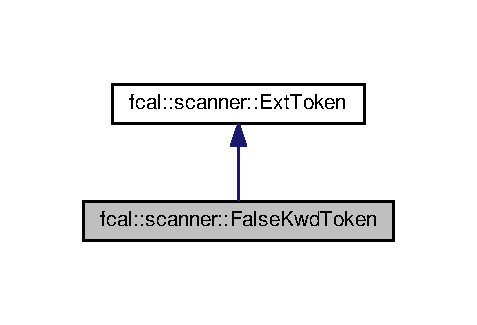
\includegraphics[width=229pt]{classfcal_1_1scanner_1_1FalseKwdToken__inherit__graph}
\end{center}
\end{figure}


Collaboration diagram for fcal\+:\+:scanner\+:\+:False\+Kwd\+Token\+:\nopagebreak
\begin{figure}[H]
\begin{center}
\leavevmode
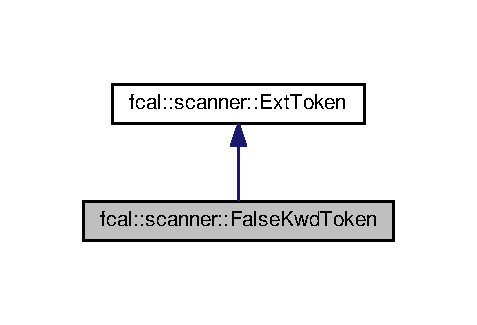
\includegraphics[width=229pt]{classfcal_1_1scanner_1_1FalseKwdToken__coll__graph}
\end{center}
\end{figure}
\subsection*{Public Member Functions}
\begin{DoxyCompactItemize}
\item 
{\bfseries False\+Kwd\+Token} (\hyperlink{classfcal_1_1parser_1_1Parser}{parser\+::\+Parser} $\ast$p, \hyperlink{classfcal_1_1scanner_1_1Token}{Token} $\ast$t)\hypertarget{classfcal_1_1scanner_1_1FalseKwdToken_ac35ad99acd8ed526d7e7a5d5216b060e}{}\label{classfcal_1_1scanner_1_1FalseKwdToken_ac35ad99acd8ed526d7e7a5d5216b060e}

\item 
\hyperlink{classfcal_1_1parser_1_1ParseResult}{parser\+::\+Parse\+Result} {\bfseries nud} ()\hypertarget{classfcal_1_1scanner_1_1FalseKwdToken_a57566622065242fe629d5f991022cdac}{}\label{classfcal_1_1scanner_1_1FalseKwdToken_a57566622065242fe629d5f991022cdac}

\item 
std\+::string {\bfseries description} ()\hypertarget{classfcal_1_1scanner_1_1FalseKwdToken_ad03d22a5baf8377d409dcae104cfc997}{}\label{classfcal_1_1scanner_1_1FalseKwdToken_ad03d22a5baf8377d409dcae104cfc997}

\end{DoxyCompactItemize}
\subsection*{Additional Inherited Members}


The documentation for this class was generated from the following file\+:\begin{DoxyCompactItemize}
\item 
include/ext\+\_\+token.\+h\end{DoxyCompactItemize}

\hypertarget{classfcal_1_1scanner_1_1FloatConstToken}{}\section{fcal\+:\+:scanner\+:\+:Float\+Const\+Token Class Reference}
\label{classfcal_1_1scanner_1_1FloatConstToken}\index{fcal\+::scanner\+::\+Float\+Const\+Token@{fcal\+::scanner\+::\+Float\+Const\+Token}}


Inheritance diagram for fcal\+:\+:scanner\+:\+:Float\+Const\+Token\+:\nopagebreak
\begin{figure}[H]
\begin{center}
\leavevmode
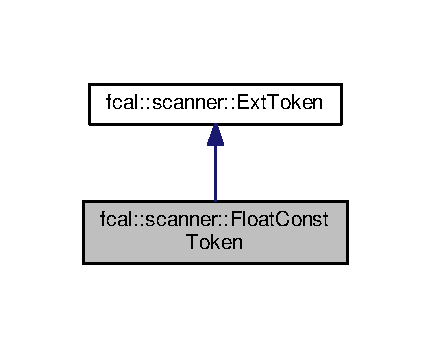
\includegraphics[width=207pt]{classfcal_1_1scanner_1_1FloatConstToken__inherit__graph}
\end{center}
\end{figure}


Collaboration diagram for fcal\+:\+:scanner\+:\+:Float\+Const\+Token\+:\nopagebreak
\begin{figure}[H]
\begin{center}
\leavevmode
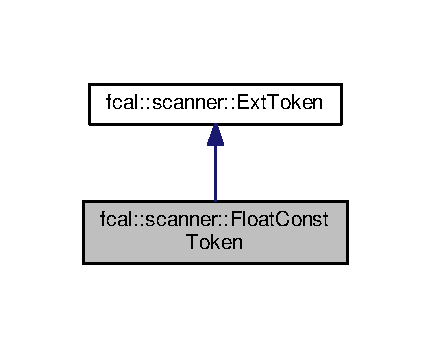
\includegraphics[width=207pt]{classfcal_1_1scanner_1_1FloatConstToken__coll__graph}
\end{center}
\end{figure}
\subsection*{Public Member Functions}
\begin{DoxyCompactItemize}
\item 
{\bfseries Float\+Const\+Token} (\hyperlink{classfcal_1_1parser_1_1Parser}{parser\+::\+Parser} $\ast$p, \hyperlink{classfcal_1_1scanner_1_1Token}{Token} $\ast$t)\hypertarget{classfcal_1_1scanner_1_1FloatConstToken_a715ecedd2f42b7fbcfbf564dad7909fc}{}\label{classfcal_1_1scanner_1_1FloatConstToken_a715ecedd2f42b7fbcfbf564dad7909fc}

\item 
\hyperlink{classfcal_1_1parser_1_1ParseResult}{parser\+::\+Parse\+Result} {\bfseries nud} ()\hypertarget{classfcal_1_1scanner_1_1FloatConstToken_a7ceca1dc6b064daf39e7250d8d93a9ce}{}\label{classfcal_1_1scanner_1_1FloatConstToken_a7ceca1dc6b064daf39e7250d8d93a9ce}

\item 
std\+::string {\bfseries description} ()\hypertarget{classfcal_1_1scanner_1_1FloatConstToken_ac98711e11205722a389fc19682183286}{}\label{classfcal_1_1scanner_1_1FloatConstToken_ac98711e11205722a389fc19682183286}

\end{DoxyCompactItemize}
\subsection*{Additional Inherited Members}


The documentation for this class was generated from the following file\+:\begin{DoxyCompactItemize}
\item 
include/ext\+\_\+token.\+h\end{DoxyCompactItemize}

\hypertarget{classfcal_1_1scanner_1_1ForwardSlashToken}{}\section{fcal\+:\+:scanner\+:\+:Forward\+Slash\+Token Class Reference}
\label{classfcal_1_1scanner_1_1ForwardSlashToken}\index{fcal\+::scanner\+::\+Forward\+Slash\+Token@{fcal\+::scanner\+::\+Forward\+Slash\+Token}}


Inheritance diagram for fcal\+:\+:scanner\+:\+:Forward\+Slash\+Token\+:\nopagebreak
\begin{figure}[H]
\begin{center}
\leavevmode
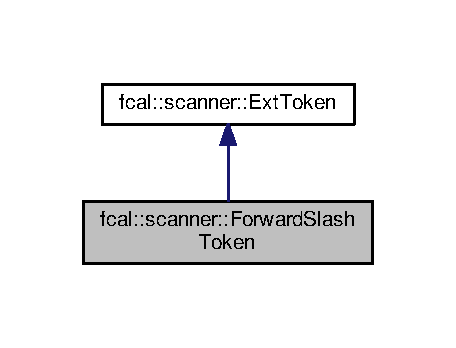
\includegraphics[width=219pt]{classfcal_1_1scanner_1_1ForwardSlashToken__inherit__graph}
\end{center}
\end{figure}


Collaboration diagram for fcal\+:\+:scanner\+:\+:Forward\+Slash\+Token\+:\nopagebreak
\begin{figure}[H]
\begin{center}
\leavevmode
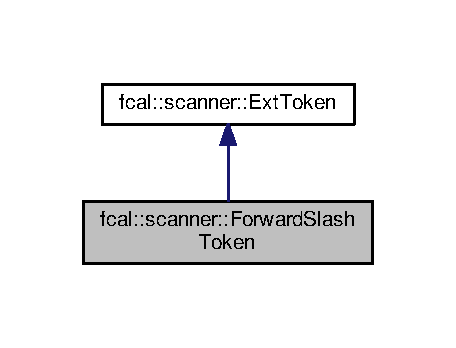
\includegraphics[width=219pt]{classfcal_1_1scanner_1_1ForwardSlashToken__coll__graph}
\end{center}
\end{figure}
\subsection*{Public Member Functions}
\begin{DoxyCompactItemize}
\item 
{\bfseries Forward\+Slash\+Token} (\hyperlink{classfcal_1_1parser_1_1Parser}{parser\+::\+Parser} $\ast$p, \hyperlink{classfcal_1_1scanner_1_1Token}{Token} $\ast$t)\hypertarget{classfcal_1_1scanner_1_1ForwardSlashToken_a78339cc748c46b86c73945ea345e6e1d}{}\label{classfcal_1_1scanner_1_1ForwardSlashToken_a78339cc748c46b86c73945ea345e6e1d}

\item 
\hyperlink{classfcal_1_1parser_1_1ParseResult}{parser\+::\+Parse\+Result} {\bfseries led} (\hyperlink{classfcal_1_1parser_1_1ParseResult}{parser\+::\+Parse\+Result} left)\hypertarget{classfcal_1_1scanner_1_1ForwardSlashToken_a75ba06718e3faa1d53c62182d0f7b1db}{}\label{classfcal_1_1scanner_1_1ForwardSlashToken_a75ba06718e3faa1d53c62182d0f7b1db}

\item 
std\+::string {\bfseries description} ()\hypertarget{classfcal_1_1scanner_1_1ForwardSlashToken_a04d39d9ea4cbb704862d33cb447de83b}{}\label{classfcal_1_1scanner_1_1ForwardSlashToken_a04d39d9ea4cbb704862d33cb447de83b}

\item 
int {\bfseries lbp} ()\hypertarget{classfcal_1_1scanner_1_1ForwardSlashToken_ae2c4a56a7c81f1f9d697ccca1e95c153}{}\label{classfcal_1_1scanner_1_1ForwardSlashToken_ae2c4a56a7c81f1f9d697ccca1e95c153}

\end{DoxyCompactItemize}
\subsection*{Additional Inherited Members}


The documentation for this class was generated from the following file\+:\begin{DoxyCompactItemize}
\item 
include/ext\+\_\+token.\+h\end{DoxyCompactItemize}

\hypertarget{classfcal_1_1ast_1_1IfElseStmt}{}\section{fcal\+:\+:ast\+:\+:If\+Else\+Stmt Class Reference}
\label{classfcal_1_1ast_1_1IfElseStmt}\index{fcal\+::ast\+::\+If\+Else\+Stmt@{fcal\+::ast\+::\+If\+Else\+Stmt}}


The \hyperlink{classfcal_1_1ast_1_1IfElseStmt}{If\+Else\+Stmt} class inherits directly from the abstract \hyperlink{classfcal_1_1ast_1_1Stmt}{Stmt} parent class.  




{\ttfamily \#include $<$ast.\+h$>$}



Inheritance diagram for fcal\+:\+:ast\+:\+:If\+Else\+Stmt\+:\nopagebreak
\begin{figure}[H]
\begin{center}
\leavevmode
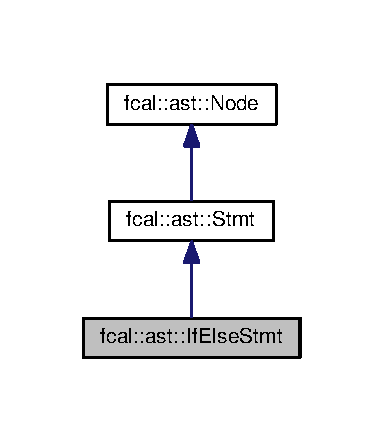
\includegraphics[width=184pt]{classfcal_1_1ast_1_1IfElseStmt__inherit__graph}
\end{center}
\end{figure}


Collaboration diagram for fcal\+:\+:ast\+:\+:If\+Else\+Stmt\+:\nopagebreak
\begin{figure}[H]
\begin{center}
\leavevmode
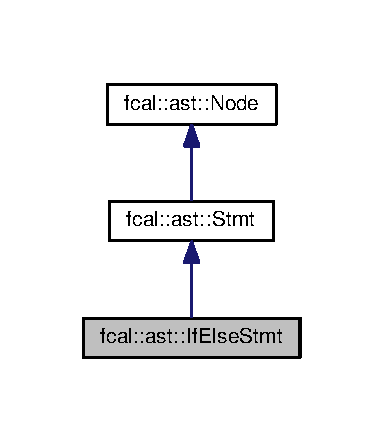
\includegraphics[width=184pt]{classfcal_1_1ast_1_1IfElseStmt__coll__graph}
\end{center}
\end{figure}
\subsection*{Public Member Functions}
\begin{DoxyCompactItemize}
\item 
\hyperlink{classfcal_1_1ast_1_1IfElseStmt_adf51b8907ed61b1608e5fe70824471e8}{If\+Else\+Stmt} (\hyperlink{classfcal_1_1ast_1_1Expr}{Expr} $\ast$expr, \hyperlink{classfcal_1_1ast_1_1Stmt}{Stmt} $\ast$stmt, \hyperlink{classfcal_1_1ast_1_1Stmt}{Stmt} $\ast$stmt2)
\item 
std\+::string \hyperlink{classfcal_1_1ast_1_1IfElseStmt_a58584903e7e9480773ca5be804342721}{unparse} ()
\begin{DoxyCompactList}\small\item\em \hyperlink{classfcal_1_1ast_1_1IfElseStmt}{If\+Else\+Stmt} unparse method() \end{DoxyCompactList}\item 
std\+::string {\bfseries cpp\+\_\+code} ()\hypertarget{classfcal_1_1ast_1_1IfElseStmt_a5339619d1f29800558f735cb6cb99681}{}\label{classfcal_1_1ast_1_1IfElseStmt_a5339619d1f29800558f735cb6cb99681}

\end{DoxyCompactItemize}


\subsection{Detailed Description}
The \hyperlink{classfcal_1_1ast_1_1IfElseStmt}{If\+Else\+Stmt} class inherits directly from the abstract \hyperlink{classfcal_1_1ast_1_1Stmt}{Stmt} parent class. 

\subsection{Constructor \& Destructor Documentation}
\index{fcal\+::ast\+::\+If\+Else\+Stmt@{fcal\+::ast\+::\+If\+Else\+Stmt}!If\+Else\+Stmt@{If\+Else\+Stmt}}
\index{If\+Else\+Stmt@{If\+Else\+Stmt}!fcal\+::ast\+::\+If\+Else\+Stmt@{fcal\+::ast\+::\+If\+Else\+Stmt}}
\subsubsection[{\texorpdfstring{If\+Else\+Stmt(\+Expr $\ast$expr, Stmt $\ast$stmt, Stmt $\ast$stmt2)}{IfElseStmt(Expr *expr, Stmt *stmt, Stmt *stmt2)}}]{\setlength{\rightskip}{0pt plus 5cm}fcal\+::ast\+::\+If\+Else\+Stmt\+::\+If\+Else\+Stmt (
\begin{DoxyParamCaption}
\item[{{\bf Expr} $\ast$}]{expr, }
\item[{{\bf Stmt} $\ast$}]{stmt, }
\item[{{\bf Stmt} $\ast$}]{stmt2}
\end{DoxyParamCaption}
)\hspace{0.3cm}{\ttfamily [inline]}, {\ttfamily [explicit]}}\hypertarget{classfcal_1_1ast_1_1IfElseStmt_adf51b8907ed61b1608e5fe70824471e8}{}\label{classfcal_1_1ast_1_1IfElseStmt_adf51b8907ed61b1608e5fe70824471e8}
\hyperlink{classfcal_1_1ast_1_1IfElseStmt}{If\+Else\+Stmt} production class takes the parameters\+: $\ast$expr, $\ast$stmt and $\ast$stmt2 
\begin{DoxyParams}{Parameters}
{\em $\ast$expr} & expression of the if statement \\
\hline
{\em $\ast$stmt} & statement of the then clause \\
\hline
{\em $\ast$stmt2} & statement of the else clause \\
\hline
\end{DoxyParams}


\subsection{Member Function Documentation}
\index{fcal\+::ast\+::\+If\+Else\+Stmt@{fcal\+::ast\+::\+If\+Else\+Stmt}!unparse@{unparse}}
\index{unparse@{unparse}!fcal\+::ast\+::\+If\+Else\+Stmt@{fcal\+::ast\+::\+If\+Else\+Stmt}}
\subsubsection[{\texorpdfstring{unparse()}{unparse()}}]{\setlength{\rightskip}{0pt plus 5cm}std\+::string fcal\+::ast\+::\+If\+Else\+Stmt\+::unparse (
\begin{DoxyParamCaption}
{}
\end{DoxyParamCaption}
)\hspace{0.3cm}{\ttfamily [virtual]}}\hypertarget{classfcal_1_1ast_1_1IfElseStmt_a58584903e7e9480773ca5be804342721}{}\label{classfcal_1_1ast_1_1IfElseStmt_a58584903e7e9480773ca5be804342721}


\hyperlink{classfcal_1_1ast_1_1IfElseStmt}{If\+Else\+Stmt} unparse method() 

\hyperlink{classfcal_1_1ast_1_1IfElseStmt}{If\+Else\+Stmt} \hyperlink{classfcal_1_1ast_1_1IfElseStmt_a58584903e7e9480773ca5be804342721}{unparse()} returns the expr\+\_\+, stmt\+\_\+ and stmt2\+\_\+ parameters. 

Implements \hyperlink{classfcal_1_1ast_1_1Node_a81865f5a1df593708a39bf492952742a}{fcal\+::ast\+::\+Node}.



The documentation for this class was generated from the following files\+:\begin{DoxyCompactItemize}
\item 
include/ast.\+h\item 
src/ast.\+cc\end{DoxyCompactItemize}

\hypertarget{classfcal_1_1ast_1_1IfExpr}{}\section{fcal\+:\+:ast\+:\+:If\+Expr Class Reference}
\label{classfcal_1_1ast_1_1IfExpr}\index{fcal\+::ast\+::\+If\+Expr@{fcal\+::ast\+::\+If\+Expr}}


The \hyperlink{classfcal_1_1ast_1_1IfExpr}{If\+Expr} class inherits directly from the abstract \hyperlink{classfcal_1_1ast_1_1Expr}{Expr} class.  




{\ttfamily \#include $<$ast.\+h$>$}



Inheritance diagram for fcal\+:\+:ast\+:\+:If\+Expr\+:
\nopagebreak
\begin{figure}[H]
\begin{center}
\leavevmode
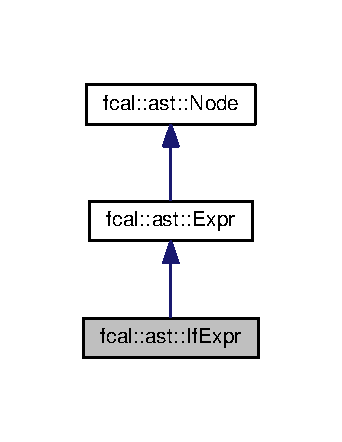
\includegraphics[width=164pt]{classfcal_1_1ast_1_1IfExpr__inherit__graph}
\end{center}
\end{figure}


Collaboration diagram for fcal\+:\+:ast\+:\+:If\+Expr\+:
\nopagebreak
\begin{figure}[H]
\begin{center}
\leavevmode
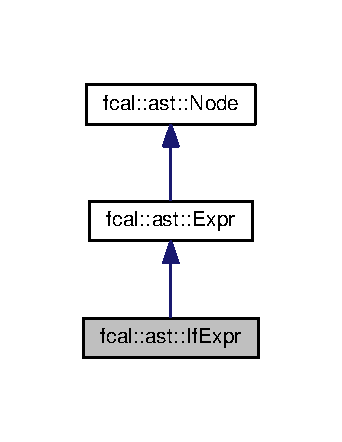
\includegraphics[width=164pt]{classfcal_1_1ast_1_1IfExpr__coll__graph}
\end{center}
\end{figure}
\subsection*{Public Member Functions}
\begin{DoxyCompactItemize}
\item 
\hyperlink{classfcal_1_1ast_1_1IfExpr_a96d71744e60f8075805e269ad01599f4}{If\+Expr} (\hyperlink{classfcal_1_1ast_1_1Expr}{Expr} $\ast$expr, \hyperlink{classfcal_1_1ast_1_1Expr}{Expr} $\ast$expr2, \hyperlink{classfcal_1_1ast_1_1Expr}{Expr} $\ast$expr3)
\item 
std\+::string \hyperlink{classfcal_1_1ast_1_1IfExpr_a4092cf20150a2cde02364d4c7233e558}{unparse} ()
\begin{DoxyCompactList}\small\item\em \hyperlink{classfcal_1_1ast_1_1IfExpr}{If\+Expr} \hyperlink{classfcal_1_1ast_1_1IfExpr_a4092cf20150a2cde02364d4c7233e558}{unparse()} method. \end{DoxyCompactList}\item 
std\+::string {\bfseries cpp\+\_\+code} ()\hypertarget{classfcal_1_1ast_1_1IfExpr_a8d6e41c15a9586eae9b440ef7a1c80ea}{}\label{classfcal_1_1ast_1_1IfExpr_a8d6e41c15a9586eae9b440ef7a1c80ea}

\end{DoxyCompactItemize}


\subsection{Detailed Description}
The \hyperlink{classfcal_1_1ast_1_1IfExpr}{If\+Expr} class inherits directly from the abstract \hyperlink{classfcal_1_1ast_1_1Expr}{Expr} class. 

\subsection{Constructor \& Destructor Documentation}
\index{fcal\+::ast\+::\+If\+Expr@{fcal\+::ast\+::\+If\+Expr}!If\+Expr@{If\+Expr}}
\index{If\+Expr@{If\+Expr}!fcal\+::ast\+::\+If\+Expr@{fcal\+::ast\+::\+If\+Expr}}
\subsubsection[{\texorpdfstring{If\+Expr(\+Expr $\ast$expr, Expr $\ast$expr2, Expr $\ast$expr3)}{IfExpr(Expr *expr, Expr *expr2, Expr *expr3)}}]{\setlength{\rightskip}{0pt plus 5cm}fcal\+::ast\+::\+If\+Expr\+::\+If\+Expr (
\begin{DoxyParamCaption}
\item[{{\bf Expr} $\ast$}]{expr, }
\item[{{\bf Expr} $\ast$}]{expr2, }
\item[{{\bf Expr} $\ast$}]{expr3}
\end{DoxyParamCaption}
)\hspace{0.3cm}{\ttfamily [inline]}, {\ttfamily [explicit]}}\hypertarget{classfcal_1_1ast_1_1IfExpr_a96d71744e60f8075805e269ad01599f4}{}\label{classfcal_1_1ast_1_1IfExpr_a96d71744e60f8075805e269ad01599f4}
\hyperlink{classfcal_1_1ast_1_1IfExpr}{If\+Expr} production rules take the paramters\+: $\ast$expr, $\ast$expr2 and $\ast$expr3 
\begin{DoxyParams}{Parameters}
{\em $\ast$expr} & is the if expression \\
\hline
{\em $\ast$expr2} & is the then expression \\
\hline
{\em $\ast$expr3} & is the else expression \\
\hline
\end{DoxyParams}


\subsection{Member Function Documentation}
\index{fcal\+::ast\+::\+If\+Expr@{fcal\+::ast\+::\+If\+Expr}!unparse@{unparse}}
\index{unparse@{unparse}!fcal\+::ast\+::\+If\+Expr@{fcal\+::ast\+::\+If\+Expr}}
\subsubsection[{\texorpdfstring{unparse()}{unparse()}}]{\setlength{\rightskip}{0pt plus 5cm}std\+::string fcal\+::ast\+::\+If\+Expr\+::unparse (
\begin{DoxyParamCaption}
{}
\end{DoxyParamCaption}
)\hspace{0.3cm}{\ttfamily [virtual]}}\hypertarget{classfcal_1_1ast_1_1IfExpr_a4092cf20150a2cde02364d4c7233e558}{}\label{classfcal_1_1ast_1_1IfExpr_a4092cf20150a2cde02364d4c7233e558}


\hyperlink{classfcal_1_1ast_1_1IfExpr}{If\+Expr} \hyperlink{classfcal_1_1ast_1_1IfExpr_a4092cf20150a2cde02364d4c7233e558}{unparse()} method. 

\hyperlink{classfcal_1_1ast_1_1IfExpr}{If\+Expr} returns expr\+\_\+, expr2\+\_\+ and expr3\+\_\+ paramters. 

Implements \hyperlink{classfcal_1_1ast_1_1Node_a81865f5a1df593708a39bf492952742a}{fcal\+::ast\+::\+Node}.



The documentation for this class was generated from the following files\+:\begin{DoxyCompactItemize}
\item 
include/ast.\+h\item 
src/ast.\+cc\end{DoxyCompactItemize}

\hypertarget{classfcal_1_1ast_1_1IfStmt}{}\section{fcal\+:\+:ast\+:\+:If\+Stmt Class Reference}
\label{classfcal_1_1ast_1_1IfStmt}\index{fcal\+::ast\+::\+If\+Stmt@{fcal\+::ast\+::\+If\+Stmt}}


The \hyperlink{classfcal_1_1ast_1_1IfStmt}{If\+Stmt} class inherits directly from the abstract \hyperlink{classfcal_1_1ast_1_1Stmt}{Stmt} parent class.  




{\ttfamily \#include $<$ast.\+h$>$}



Inheritance diagram for fcal\+:\+:ast\+:\+:If\+Stmt\+:
\nopagebreak
\begin{figure}[H]
\begin{center}
\leavevmode
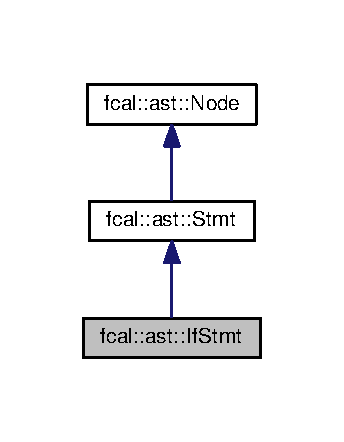
\includegraphics[width=165pt]{classfcal_1_1ast_1_1IfStmt__inherit__graph}
\end{center}
\end{figure}


Collaboration diagram for fcal\+:\+:ast\+:\+:If\+Stmt\+:
\nopagebreak
\begin{figure}[H]
\begin{center}
\leavevmode
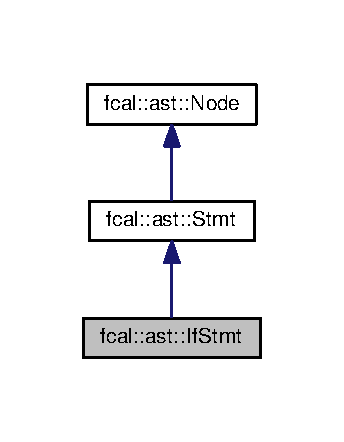
\includegraphics[width=165pt]{classfcal_1_1ast_1_1IfStmt__coll__graph}
\end{center}
\end{figure}
\subsection*{Public Member Functions}
\begin{DoxyCompactItemize}
\item 
\hyperlink{classfcal_1_1ast_1_1IfStmt_aaf938559e1c0ebedd6b670a88323af19}{If\+Stmt} (\hyperlink{classfcal_1_1ast_1_1Expr}{Expr} $\ast$expr, \hyperlink{classfcal_1_1ast_1_1Stmt}{Stmt} $\ast$stmt)
\item 
std\+::string \hyperlink{classfcal_1_1ast_1_1IfStmt_acf7d0fbe7a9ff597216a23992f603062}{unparse} ()
\begin{DoxyCompactList}\small\item\em \hyperlink{classfcal_1_1ast_1_1IfStmt}{If\+Stmt} \hyperlink{classfcal_1_1ast_1_1IfStmt_acf7d0fbe7a9ff597216a23992f603062}{unparse()} method. \end{DoxyCompactList}\item 
std\+::string {\bfseries cpp\+\_\+code} ()\hypertarget{classfcal_1_1ast_1_1IfStmt_aff4861d1e02ebf4de6a8ae65e5473fc5}{}\label{classfcal_1_1ast_1_1IfStmt_aff4861d1e02ebf4de6a8ae65e5473fc5}

\end{DoxyCompactItemize}


\subsection{Detailed Description}
The \hyperlink{classfcal_1_1ast_1_1IfStmt}{If\+Stmt} class inherits directly from the abstract \hyperlink{classfcal_1_1ast_1_1Stmt}{Stmt} parent class. 

\subsection{Constructor \& Destructor Documentation}
\index{fcal\+::ast\+::\+If\+Stmt@{fcal\+::ast\+::\+If\+Stmt}!If\+Stmt@{If\+Stmt}}
\index{If\+Stmt@{If\+Stmt}!fcal\+::ast\+::\+If\+Stmt@{fcal\+::ast\+::\+If\+Stmt}}
\subsubsection[{\texorpdfstring{If\+Stmt(\+Expr $\ast$expr, Stmt $\ast$stmt)}{IfStmt(Expr *expr, Stmt *stmt)}}]{\setlength{\rightskip}{0pt plus 5cm}fcal\+::ast\+::\+If\+Stmt\+::\+If\+Stmt (
\begin{DoxyParamCaption}
\item[{{\bf Expr} $\ast$}]{expr, }
\item[{{\bf Stmt} $\ast$}]{stmt}
\end{DoxyParamCaption}
)\hspace{0.3cm}{\ttfamily [inline]}, {\ttfamily [explicit]}}\hypertarget{classfcal_1_1ast_1_1IfStmt_aaf938559e1c0ebedd6b670a88323af19}{}\label{classfcal_1_1ast_1_1IfStmt_aaf938559e1c0ebedd6b670a88323af19}
\hyperlink{classfcal_1_1ast_1_1IfStmt}{If\+Stmt} production class takes the parameters\+: $\ast$expr and $\ast$stmt 
\begin{DoxyParams}{Parameters}
{\em $\ast$expr} & expression of the if statement \\
\hline
{\em $\ast$stmt} & statement of the then clause \\
\hline
\end{DoxyParams}


\subsection{Member Function Documentation}
\index{fcal\+::ast\+::\+If\+Stmt@{fcal\+::ast\+::\+If\+Stmt}!unparse@{unparse}}
\index{unparse@{unparse}!fcal\+::ast\+::\+If\+Stmt@{fcal\+::ast\+::\+If\+Stmt}}
\subsubsection[{\texorpdfstring{unparse()}{unparse()}}]{\setlength{\rightskip}{0pt plus 5cm}std\+::string fcal\+::ast\+::\+If\+Stmt\+::unparse (
\begin{DoxyParamCaption}
{}
\end{DoxyParamCaption}
)\hspace{0.3cm}{\ttfamily [virtual]}}\hypertarget{classfcal_1_1ast_1_1IfStmt_acf7d0fbe7a9ff597216a23992f603062}{}\label{classfcal_1_1ast_1_1IfStmt_acf7d0fbe7a9ff597216a23992f603062}


\hyperlink{classfcal_1_1ast_1_1IfStmt}{If\+Stmt} \hyperlink{classfcal_1_1ast_1_1IfStmt_acf7d0fbe7a9ff597216a23992f603062}{unparse()} method. 

\hyperlink{classfcal_1_1ast_1_1IfStmt}{If\+Stmt} \hyperlink{classfcal_1_1ast_1_1IfStmt_acf7d0fbe7a9ff597216a23992f603062}{unparse()} returns the expr\+\_\+ and stmt\+\_\+ parameters. 

Implements \hyperlink{classfcal_1_1ast_1_1Node_a81865f5a1df593708a39bf492952742a}{fcal\+::ast\+::\+Node}.



The documentation for this class was generated from the following files\+:\begin{DoxyCompactItemize}
\item 
include/ast.\+h\item 
src/ast.\+cc\end{DoxyCompactItemize}

\hypertarget{classfcal_1_1scanner_1_1IfToken}{}\section{fcal\+:\+:scanner\+:\+:If\+Token Class Reference}
\label{classfcal_1_1scanner_1_1IfToken}\index{fcal\+::scanner\+::\+If\+Token@{fcal\+::scanner\+::\+If\+Token}}


Inheritance diagram for fcal\+:\+:scanner\+:\+:If\+Token\+:\nopagebreak
\begin{figure}[H]
\begin{center}
\leavevmode
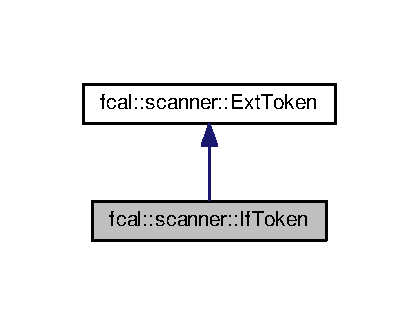
\includegraphics[width=201pt]{classfcal_1_1scanner_1_1IfToken__inherit__graph}
\end{center}
\end{figure}


Collaboration diagram for fcal\+:\+:scanner\+:\+:If\+Token\+:\nopagebreak
\begin{figure}[H]
\begin{center}
\leavevmode
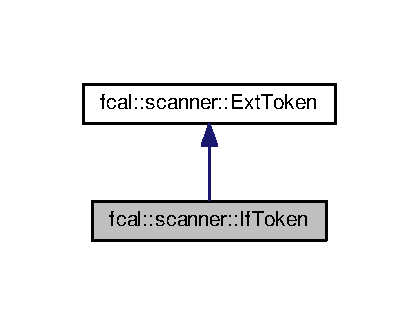
\includegraphics[width=201pt]{classfcal_1_1scanner_1_1IfToken__coll__graph}
\end{center}
\end{figure}
\subsection*{Public Member Functions}
\begin{DoxyCompactItemize}
\item 
{\bfseries If\+Token} (\hyperlink{classfcal_1_1parser_1_1Parser}{parser\+::\+Parser} $\ast$p, \hyperlink{classfcal_1_1scanner_1_1Token}{Token} $\ast$t)\hypertarget{classfcal_1_1scanner_1_1IfToken_ab62190e056e132f94f99077fd48049fc}{}\label{classfcal_1_1scanner_1_1IfToken_ab62190e056e132f94f99077fd48049fc}

\item 
\hyperlink{classfcal_1_1parser_1_1ParseResult}{parser\+::\+Parse\+Result} {\bfseries nud} ()\hypertarget{classfcal_1_1scanner_1_1IfToken_a66e666cbade5d1be24d0639dad88a594}{}\label{classfcal_1_1scanner_1_1IfToken_a66e666cbade5d1be24d0639dad88a594}

\item 
std\+::string {\bfseries description} ()\hypertarget{classfcal_1_1scanner_1_1IfToken_a76c60330e996fab7bbcaaab1f825d62c}{}\label{classfcal_1_1scanner_1_1IfToken_a76c60330e996fab7bbcaaab1f825d62c}

\item 
int {\bfseries lbp} ()\hypertarget{classfcal_1_1scanner_1_1IfToken_a8ef9ce247acf496793ef3cecafea1c42}{}\label{classfcal_1_1scanner_1_1IfToken_a8ef9ce247acf496793ef3cecafea1c42}

\end{DoxyCompactItemize}
\subsection*{Additional Inherited Members}


The documentation for this class was generated from the following file\+:\begin{DoxyCompactItemize}
\item 
include/ext\+\_\+token.\+h\end{DoxyCompactItemize}

\hypertarget{classfcal_1_1scanner_1_1IntConstToken}{}\section{fcal\+:\+:scanner\+:\+:Int\+Const\+Token Class Reference}
\label{classfcal_1_1scanner_1_1IntConstToken}\index{fcal\+::scanner\+::\+Int\+Const\+Token@{fcal\+::scanner\+::\+Int\+Const\+Token}}


Inheritance diagram for fcal\+:\+:scanner\+:\+:Int\+Const\+Token\+:
\nopagebreak
\begin{figure}[H]
\begin{center}
\leavevmode
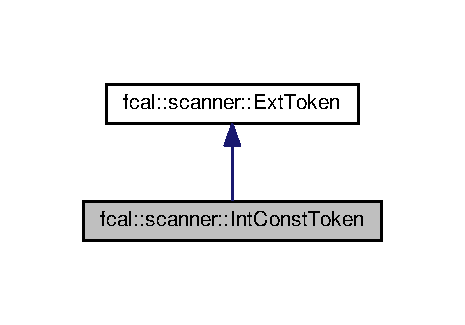
\includegraphics[width=223pt]{classfcal_1_1scanner_1_1IntConstToken__inherit__graph}
\end{center}
\end{figure}


Collaboration diagram for fcal\+:\+:scanner\+:\+:Int\+Const\+Token\+:
\nopagebreak
\begin{figure}[H]
\begin{center}
\leavevmode
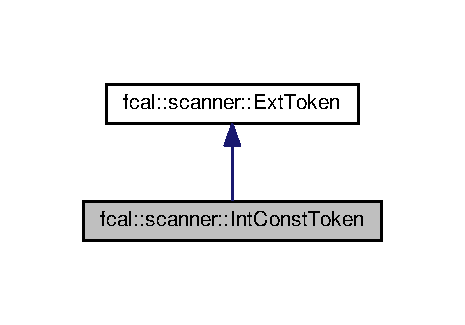
\includegraphics[width=223pt]{classfcal_1_1scanner_1_1IntConstToken__coll__graph}
\end{center}
\end{figure}
\subsection*{Public Member Functions}
\begin{DoxyCompactItemize}
\item 
{\bfseries Int\+Const\+Token} (\hyperlink{classfcal_1_1parser_1_1Parser}{parser\+::\+Parser} $\ast$p, \hyperlink{classfcal_1_1scanner_1_1Token}{Token} $\ast$t)\hypertarget{classfcal_1_1scanner_1_1IntConstToken_a2846b99b9b48717e35d81446618eb924}{}\label{classfcal_1_1scanner_1_1IntConstToken_a2846b99b9b48717e35d81446618eb924}

\item 
\hyperlink{classfcal_1_1parser_1_1ParseResult}{parser\+::\+Parse\+Result} {\bfseries nud} ()\hypertarget{classfcal_1_1scanner_1_1IntConstToken_aede9ed23780dbb33a7852b3ecf6183da}{}\label{classfcal_1_1scanner_1_1IntConstToken_aede9ed23780dbb33a7852b3ecf6183da}

\item 
std\+::string {\bfseries description} ()\hypertarget{classfcal_1_1scanner_1_1IntConstToken_a9359c997cac9cf57a5c7debc6a1811ab}{}\label{classfcal_1_1scanner_1_1IntConstToken_a9359c997cac9cf57a5c7debc6a1811ab}

\end{DoxyCompactItemize}
\subsection*{Additional Inherited Members}


The documentation for this class was generated from the following file\+:\begin{DoxyCompactItemize}
\item 
include/ext\+\_\+token.\+h\end{DoxyCompactItemize}

\hypertarget{classfcal_1_1scanner_1_1LeftParenToken}{}\section{fcal\+:\+:scanner\+:\+:Left\+Paren\+Token Class Reference}
\label{classfcal_1_1scanner_1_1LeftParenToken}\index{fcal\+::scanner\+::\+Left\+Paren\+Token@{fcal\+::scanner\+::\+Left\+Paren\+Token}}


Inheritance diagram for fcal\+:\+:scanner\+:\+:Left\+Paren\+Token\+:
\nopagebreak
\begin{figure}[H]
\begin{center}
\leavevmode
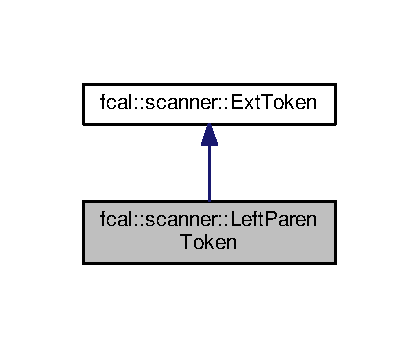
\includegraphics[width=201pt]{classfcal_1_1scanner_1_1LeftParenToken__inherit__graph}
\end{center}
\end{figure}


Collaboration diagram for fcal\+:\+:scanner\+:\+:Left\+Paren\+Token\+:
\nopagebreak
\begin{figure}[H]
\begin{center}
\leavevmode
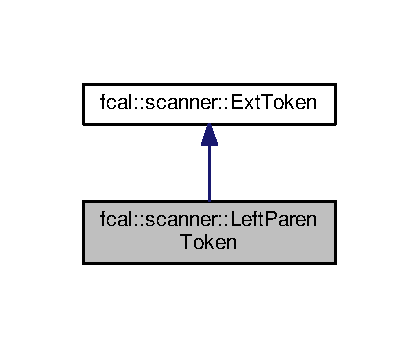
\includegraphics[width=201pt]{classfcal_1_1scanner_1_1LeftParenToken__coll__graph}
\end{center}
\end{figure}
\subsection*{Public Member Functions}
\begin{DoxyCompactItemize}
\item 
{\bfseries Left\+Paren\+Token} (\hyperlink{classfcal_1_1parser_1_1Parser}{parser\+::\+Parser} $\ast$p, \hyperlink{classfcal_1_1scanner_1_1Token}{Token} $\ast$t)\hypertarget{classfcal_1_1scanner_1_1LeftParenToken_a306e81a052bdff9c4e9fb4912e0732ee}{}\label{classfcal_1_1scanner_1_1LeftParenToken_a306e81a052bdff9c4e9fb4912e0732ee}

\item 
\hyperlink{classfcal_1_1parser_1_1ParseResult}{parser\+::\+Parse\+Result} {\bfseries nud} ()\hypertarget{classfcal_1_1scanner_1_1LeftParenToken_a793eb1dfcd6ea5546081c7cf8733534a}{}\label{classfcal_1_1scanner_1_1LeftParenToken_a793eb1dfcd6ea5546081c7cf8733534a}

\item 
std\+::string {\bfseries description} ()\hypertarget{classfcal_1_1scanner_1_1LeftParenToken_a32ea8cf7b793bb532161781f8f42113c}{}\label{classfcal_1_1scanner_1_1LeftParenToken_a32ea8cf7b793bb532161781f8f42113c}

\item 
int {\bfseries lbp} ()\hypertarget{classfcal_1_1scanner_1_1LeftParenToken_a2bfc3c31dc0fef8961d4f33a3bc81f25}{}\label{classfcal_1_1scanner_1_1LeftParenToken_a2bfc3c31dc0fef8961d4f33a3bc81f25}

\end{DoxyCompactItemize}
\subsection*{Additional Inherited Members}


The documentation for this class was generated from the following file\+:\begin{DoxyCompactItemize}
\item 
include/ext\+\_\+token.\+h\end{DoxyCompactItemize}

\hypertarget{classfcal_1_1ast_1_1LetExpr}{}\section{fcal\+:\+:ast\+:\+:Let\+Expr Class Reference}
\label{classfcal_1_1ast_1_1LetExpr}\index{fcal\+::ast\+::\+Let\+Expr@{fcal\+::ast\+::\+Let\+Expr}}


The \hyperlink{classfcal_1_1ast_1_1LetExpr}{Let\+Expr} class inherits directly from the abstract \hyperlink{classfcal_1_1ast_1_1Expr}{Expr} class.  




{\ttfamily \#include $<$ast.\+h$>$}



Inheritance diagram for fcal\+:\+:ast\+:\+:Let\+Expr\+:
\nopagebreak
\begin{figure}[H]
\begin{center}
\leavevmode
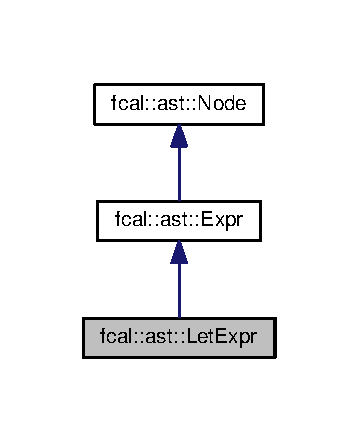
\includegraphics[width=172pt]{classfcal_1_1ast_1_1LetExpr__inherit__graph}
\end{center}
\end{figure}


Collaboration diagram for fcal\+:\+:ast\+:\+:Let\+Expr\+:
\nopagebreak
\begin{figure}[H]
\begin{center}
\leavevmode
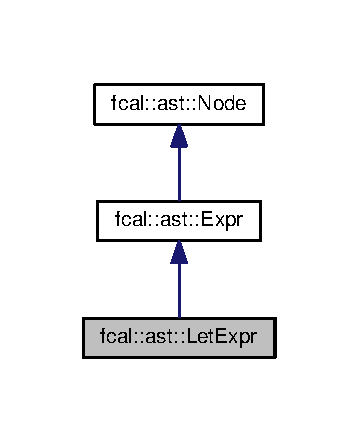
\includegraphics[width=172pt]{classfcal_1_1ast_1_1LetExpr__coll__graph}
\end{center}
\end{figure}
\subsection*{Public Member Functions}
\begin{DoxyCompactItemize}
\item 
\hyperlink{classfcal_1_1ast_1_1LetExpr_ab74edb2ea044f4a53e3aaf07ba3e692a}{Let\+Expr} (\hyperlink{classfcal_1_1ast_1_1Stmts}{Stmts} $\ast$stmts, \hyperlink{classfcal_1_1ast_1_1Expr}{Expr} $\ast$expr)
\item 
std\+::string \hyperlink{classfcal_1_1ast_1_1LetExpr_a5277bbe3510e870f65dd9158592ef6da}{unparse} ()
\begin{DoxyCompactList}\small\item\em \hyperlink{classfcal_1_1ast_1_1LetExpr}{Let\+Expr} \hyperlink{classfcal_1_1ast_1_1LetExpr_a5277bbe3510e870f65dd9158592ef6da}{unparse()} method. \end{DoxyCompactList}\item 
std\+::string {\bfseries cpp\+\_\+code} ()\hypertarget{classfcal_1_1ast_1_1LetExpr_a960972260e0f70e3baa79b10d5c0d8ce}{}\label{classfcal_1_1ast_1_1LetExpr_a960972260e0f70e3baa79b10d5c0d8ce}

\end{DoxyCompactItemize}


\subsection{Detailed Description}
The \hyperlink{classfcal_1_1ast_1_1LetExpr}{Let\+Expr} class inherits directly from the abstract \hyperlink{classfcal_1_1ast_1_1Expr}{Expr} class. 

\subsection{Constructor \& Destructor Documentation}
\index{fcal\+::ast\+::\+Let\+Expr@{fcal\+::ast\+::\+Let\+Expr}!Let\+Expr@{Let\+Expr}}
\index{Let\+Expr@{Let\+Expr}!fcal\+::ast\+::\+Let\+Expr@{fcal\+::ast\+::\+Let\+Expr}}
\subsubsection[{\texorpdfstring{Let\+Expr(\+Stmts $\ast$stmts, Expr $\ast$expr)}{LetExpr(Stmts *stmts, Expr *expr)}}]{\setlength{\rightskip}{0pt plus 5cm}fcal\+::ast\+::\+Let\+Expr\+::\+Let\+Expr (
\begin{DoxyParamCaption}
\item[{{\bf Stmts} $\ast$}]{stmts, }
\item[{{\bf Expr} $\ast$}]{expr}
\end{DoxyParamCaption}
)\hspace{0.3cm}{\ttfamily [inline]}, {\ttfamily [explicit]}}\hypertarget{classfcal_1_1ast_1_1LetExpr_ab74edb2ea044f4a53e3aaf07ba3e692a}{}\label{classfcal_1_1ast_1_1LetExpr_ab74edb2ea044f4a53e3aaf07ba3e692a}
\hyperlink{classfcal_1_1ast_1_1LetExpr}{Let\+Expr} production rules take the parameters\+: $\ast$stmts and $\ast$expr 
\begin{DoxyParams}{Parameters}
{\em $\ast$stmts} & are the statements between let and in \\
\hline
{\em $\ast$expr} & is the expression after in and before end \\
\hline
\end{DoxyParams}


\subsection{Member Function Documentation}
\index{fcal\+::ast\+::\+Let\+Expr@{fcal\+::ast\+::\+Let\+Expr}!unparse@{unparse}}
\index{unparse@{unparse}!fcal\+::ast\+::\+Let\+Expr@{fcal\+::ast\+::\+Let\+Expr}}
\subsubsection[{\texorpdfstring{unparse()}{unparse()}}]{\setlength{\rightskip}{0pt plus 5cm}std\+::string fcal\+::ast\+::\+Let\+Expr\+::unparse (
\begin{DoxyParamCaption}
{}
\end{DoxyParamCaption}
)\hspace{0.3cm}{\ttfamily [virtual]}}\hypertarget{classfcal_1_1ast_1_1LetExpr_a5277bbe3510e870f65dd9158592ef6da}{}\label{classfcal_1_1ast_1_1LetExpr_a5277bbe3510e870f65dd9158592ef6da}


\hyperlink{classfcal_1_1ast_1_1LetExpr}{Let\+Expr} \hyperlink{classfcal_1_1ast_1_1LetExpr_a5277bbe3510e870f65dd9158592ef6da}{unparse()} method. 

\hyperlink{classfcal_1_1ast_1_1LetExpr}{Let\+Expr} returns the stmts\+\_\+ and expr\+\_\+ paramters. 

Implements \hyperlink{classfcal_1_1ast_1_1Node_a81865f5a1df593708a39bf492952742a}{fcal\+::ast\+::\+Node}.



The documentation for this class was generated from the following files\+:\begin{DoxyCompactItemize}
\item 
include/ast.\+h\item 
src/ast.\+cc\end{DoxyCompactItemize}

\hypertarget{classfcal_1_1scanner_1_1LetToken}{}\section{fcal\+:\+:scanner\+:\+:Let\+Token Class Reference}
\label{classfcal_1_1scanner_1_1LetToken}\index{fcal\+::scanner\+::\+Let\+Token@{fcal\+::scanner\+::\+Let\+Token}}


Inheritance diagram for fcal\+:\+:scanner\+:\+:Let\+Token\+:\nopagebreak
\begin{figure}[H]
\begin{center}
\leavevmode
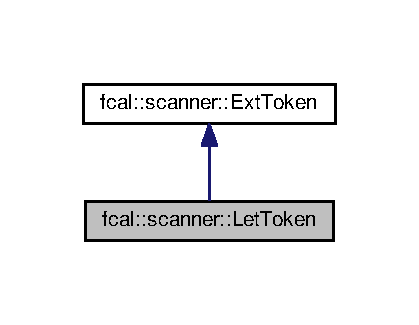
\includegraphics[width=201pt]{classfcal_1_1scanner_1_1LetToken__inherit__graph}
\end{center}
\end{figure}


Collaboration diagram for fcal\+:\+:scanner\+:\+:Let\+Token\+:\nopagebreak
\begin{figure}[H]
\begin{center}
\leavevmode
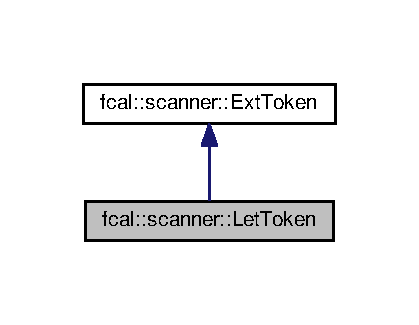
\includegraphics[width=201pt]{classfcal_1_1scanner_1_1LetToken__coll__graph}
\end{center}
\end{figure}
\subsection*{Public Member Functions}
\begin{DoxyCompactItemize}
\item 
{\bfseries Let\+Token} (\hyperlink{classfcal_1_1parser_1_1Parser}{parser\+::\+Parser} $\ast$p, \hyperlink{classfcal_1_1scanner_1_1Token}{Token} $\ast$t)\hypertarget{classfcal_1_1scanner_1_1LetToken_ad9897630e641c116602af17066086bf0}{}\label{classfcal_1_1scanner_1_1LetToken_ad9897630e641c116602af17066086bf0}

\item 
\hyperlink{classfcal_1_1parser_1_1ParseResult}{parser\+::\+Parse\+Result} {\bfseries nud} ()\hypertarget{classfcal_1_1scanner_1_1LetToken_a020d102d24a3bda7bddec7e6ccbb7f01}{}\label{classfcal_1_1scanner_1_1LetToken_a020d102d24a3bda7bddec7e6ccbb7f01}

\item 
std\+::string {\bfseries description} ()\hypertarget{classfcal_1_1scanner_1_1LetToken_aabb7ae69eea2ce5e179c26a72a479aa9}{}\label{classfcal_1_1scanner_1_1LetToken_aabb7ae69eea2ce5e179c26a72a479aa9}

\item 
int {\bfseries lbp} ()\hypertarget{classfcal_1_1scanner_1_1LetToken_abefbfa2c420b3e1214b85849d0db2e43}{}\label{classfcal_1_1scanner_1_1LetToken_abefbfa2c420b3e1214b85849d0db2e43}

\end{DoxyCompactItemize}
\subsection*{Additional Inherited Members}


The documentation for this class was generated from the following file\+:\begin{DoxyCompactItemize}
\item 
include/ext\+\_\+token.\+h\end{DoxyCompactItemize}

\hypertarget{classfcal_1_1ast_1_1MatrixDecl}{}\section{fcal\+:\+:ast\+:\+:Matrix\+Decl Class Reference}
\label{classfcal_1_1ast_1_1MatrixDecl}\index{fcal\+::ast\+::\+Matrix\+Decl@{fcal\+::ast\+::\+Matrix\+Decl}}


The \hyperlink{classfcal_1_1ast_1_1MatrixDecl}{Matrix\+Decl} class inherits directly from the abstract \hyperlink{classfcal_1_1ast_1_1Decl}{Decl} class.  




{\ttfamily \#include $<$ast.\+h$>$}



Inheritance diagram for fcal\+:\+:ast\+:\+:Matrix\+Decl\+:\nopagebreak
\begin{figure}[H]
\begin{center}
\leavevmode
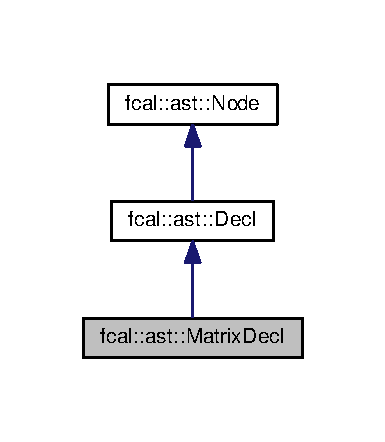
\includegraphics[width=185pt]{classfcal_1_1ast_1_1MatrixDecl__inherit__graph}
\end{center}
\end{figure}


Collaboration diagram for fcal\+:\+:ast\+:\+:Matrix\+Decl\+:\nopagebreak
\begin{figure}[H]
\begin{center}
\leavevmode
\includegraphics[width=185pt]{classfcal_1_1ast_1_1MatrixDecl__coll__graph}
\end{center}
\end{figure}
\subsection*{Public Member Functions}
\begin{DoxyCompactItemize}
\item 
\hyperlink{classfcal_1_1ast_1_1MatrixDecl_ac46452a489e1f9d3c55082468b605810}{Matrix\+Decl} (\hyperlink{classfcal_1_1ast_1_1VarName}{Var\+Name} $\ast$var\+\_\+name, \hyperlink{classfcal_1_1ast_1_1Expr}{Expr} $\ast$expr)
\item 
std\+::string \hyperlink{classfcal_1_1ast_1_1MatrixDecl_adae5ce31554a86fb0273d3d7d9258418}{unparse} ()
\begin{DoxyCompactList}\small\item\em \hyperlink{classfcal_1_1ast_1_1MatrixDecl}{Matrix\+Decl} \hyperlink{classfcal_1_1ast_1_1MatrixDecl_adae5ce31554a86fb0273d3d7d9258418}{unparse()} method. \end{DoxyCompactList}\item 
std\+::string {\bfseries cpp\+\_\+code} ()\hypertarget{classfcal_1_1ast_1_1MatrixDecl_af81d9bd3c45804445636cca2f6268811}{}\label{classfcal_1_1ast_1_1MatrixDecl_af81d9bd3c45804445636cca2f6268811}

\end{DoxyCompactItemize}


\subsection{Detailed Description}
The \hyperlink{classfcal_1_1ast_1_1MatrixDecl}{Matrix\+Decl} class inherits directly from the abstract \hyperlink{classfcal_1_1ast_1_1Decl}{Decl} class. 

\subsection{Constructor \& Destructor Documentation}
\index{fcal\+::ast\+::\+Matrix\+Decl@{fcal\+::ast\+::\+Matrix\+Decl}!Matrix\+Decl@{Matrix\+Decl}}
\index{Matrix\+Decl@{Matrix\+Decl}!fcal\+::ast\+::\+Matrix\+Decl@{fcal\+::ast\+::\+Matrix\+Decl}}
\subsubsection[{\texorpdfstring{Matrix\+Decl(\+Var\+Name $\ast$var\+\_\+name, Expr $\ast$expr)}{MatrixDecl(VarName *var_name, Expr *expr)}}]{\setlength{\rightskip}{0pt plus 5cm}fcal\+::ast\+::\+Matrix\+Decl\+::\+Matrix\+Decl (
\begin{DoxyParamCaption}
\item[{{\bf Var\+Name} $\ast$}]{var\+\_\+name, }
\item[{{\bf Expr} $\ast$}]{expr}
\end{DoxyParamCaption}
)\hspace{0.3cm}{\ttfamily [inline]}, {\ttfamily [explicit]}}\hypertarget{classfcal_1_1ast_1_1MatrixDecl_ac46452a489e1f9d3c55082468b605810}{}\label{classfcal_1_1ast_1_1MatrixDecl_ac46452a489e1f9d3c55082468b605810}
\hyperlink{classfcal_1_1ast_1_1MatrixDecl}{Matrix\+Decl} production class takes the parameters\+: $\ast$var\+\_\+name and $\ast$expr 
\begin{DoxyParams}{Parameters}
{\em $\ast$var\+\_\+name} & is the name of the variable being assigned \\
\hline
{\em $\ast$expr} & is the expression being assigned to the variable \\
\hline
\end{DoxyParams}


\subsection{Member Function Documentation}
\index{fcal\+::ast\+::\+Matrix\+Decl@{fcal\+::ast\+::\+Matrix\+Decl}!unparse@{unparse}}
\index{unparse@{unparse}!fcal\+::ast\+::\+Matrix\+Decl@{fcal\+::ast\+::\+Matrix\+Decl}}
\subsubsection[{\texorpdfstring{unparse()}{unparse()}}]{\setlength{\rightskip}{0pt plus 5cm}std\+::string fcal\+::ast\+::\+Matrix\+Decl\+::unparse (
\begin{DoxyParamCaption}
{}
\end{DoxyParamCaption}
)\hspace{0.3cm}{\ttfamily [virtual]}}\hypertarget{classfcal_1_1ast_1_1MatrixDecl_adae5ce31554a86fb0273d3d7d9258418}{}\label{classfcal_1_1ast_1_1MatrixDecl_adae5ce31554a86fb0273d3d7d9258418}


\hyperlink{classfcal_1_1ast_1_1MatrixDecl}{Matrix\+Decl} \hyperlink{classfcal_1_1ast_1_1MatrixDecl_adae5ce31554a86fb0273d3d7d9258418}{unparse()} method. 

\hyperlink{classfcal_1_1ast_1_1MatrixDecl}{Matrix\+Decl} returns var\+\_\+name\+\_\+ and expr\+\_\+. 

Implements \hyperlink{classfcal_1_1ast_1_1Node_a81865f5a1df593708a39bf492952742a}{fcal\+::ast\+::\+Node}.



The documentation for this class was generated from the following files\+:\begin{DoxyCompactItemize}
\item 
include/ast.\+h\item 
src/ast.\+cc\end{DoxyCompactItemize}

\hypertarget{classfcal_1_1ast_1_1MatrixLongDecl}{}\section{fcal\+:\+:ast\+:\+:Matrix\+Long\+Decl Class Reference}
\label{classfcal_1_1ast_1_1MatrixLongDecl}\index{fcal\+::ast\+::\+Matrix\+Long\+Decl@{fcal\+::ast\+::\+Matrix\+Long\+Decl}}


The \hyperlink{classfcal_1_1ast_1_1MatrixLongDecl}{Matrix\+Long\+Decl} class inherits directly from the abstract \hyperlink{classfcal_1_1ast_1_1Decl}{Decl} class.  




{\ttfamily \#include $<$ast.\+h$>$}



Inheritance diagram for fcal\+:\+:ast\+:\+:Matrix\+Long\+Decl\+:
\nopagebreak
\begin{figure}[H]
\begin{center}
\leavevmode
\includegraphics[width=206pt]{classfcal_1_1ast_1_1MatrixLongDecl__inherit__graph}
\end{center}
\end{figure}


Collaboration diagram for fcal\+:\+:ast\+:\+:Matrix\+Long\+Decl\+:
\nopagebreak
\begin{figure}[H]
\begin{center}
\leavevmode
\includegraphics[width=206pt]{classfcal_1_1ast_1_1MatrixLongDecl__coll__graph}
\end{center}
\end{figure}
\subsection*{Public Member Functions}
\begin{DoxyCompactItemize}
\item 
\hyperlink{classfcal_1_1ast_1_1MatrixLongDecl_a95cfff1523f2c6c7566303bf0fcfd615}{Matrix\+Long\+Decl} (\hyperlink{classfcal_1_1ast_1_1VarName}{Var\+Name} $\ast$var\+\_\+name, \hyperlink{classfcal_1_1ast_1_1Expr}{Expr} $\ast$expr, \hyperlink{classfcal_1_1ast_1_1Expr}{Expr} $\ast$expr2, \hyperlink{classfcal_1_1ast_1_1VarName}{Var\+Name} $\ast$var\+\_\+name2, \hyperlink{classfcal_1_1ast_1_1VarName}{Var\+Name} $\ast$var\+\_\+name3, \hyperlink{classfcal_1_1ast_1_1Expr}{Expr} $\ast$expr3)
\item 
std\+::string \hyperlink{classfcal_1_1ast_1_1MatrixLongDecl_addb5a0fd67a3468af9a5a512e268301e}{unparse} ()
\begin{DoxyCompactList}\small\item\em \hyperlink{classfcal_1_1ast_1_1MatrixLongDecl}{Matrix\+Long\+Decl} \hyperlink{classfcal_1_1ast_1_1MatrixLongDecl_addb5a0fd67a3468af9a5a512e268301e}{unparse()} method. \end{DoxyCompactList}\item 
std\+::string {\bfseries cpp\+\_\+code} ()\hypertarget{classfcal_1_1ast_1_1MatrixLongDecl_ab46f23586f9c5e38bd1959dd47a1e522}{}\label{classfcal_1_1ast_1_1MatrixLongDecl_ab46f23586f9c5e38bd1959dd47a1e522}

\end{DoxyCompactItemize}


\subsection{Detailed Description}
The \hyperlink{classfcal_1_1ast_1_1MatrixLongDecl}{Matrix\+Long\+Decl} class inherits directly from the abstract \hyperlink{classfcal_1_1ast_1_1Decl}{Decl} class. 

\subsection{Constructor \& Destructor Documentation}
\index{fcal\+::ast\+::\+Matrix\+Long\+Decl@{fcal\+::ast\+::\+Matrix\+Long\+Decl}!Matrix\+Long\+Decl@{Matrix\+Long\+Decl}}
\index{Matrix\+Long\+Decl@{Matrix\+Long\+Decl}!fcal\+::ast\+::\+Matrix\+Long\+Decl@{fcal\+::ast\+::\+Matrix\+Long\+Decl}}
\subsubsection[{\texorpdfstring{Matrix\+Long\+Decl(\+Var\+Name $\ast$var\+\_\+name, Expr $\ast$expr, Expr $\ast$expr2, Var\+Name $\ast$var\+\_\+name2, Var\+Name $\ast$var\+\_\+name3, Expr $\ast$expr3)}{MatrixLongDecl(VarName *var_name, Expr *expr, Expr *expr2, VarName *var_name2, VarName *var_name3, Expr *expr3)}}]{\setlength{\rightskip}{0pt plus 5cm}fcal\+::ast\+::\+Matrix\+Long\+Decl\+::\+Matrix\+Long\+Decl (
\begin{DoxyParamCaption}
\item[{{\bf Var\+Name} $\ast$}]{var\+\_\+name, }
\item[{{\bf Expr} $\ast$}]{expr, }
\item[{{\bf Expr} $\ast$}]{expr2, }
\item[{{\bf Var\+Name} $\ast$}]{var\+\_\+name2, }
\item[{{\bf Var\+Name} $\ast$}]{var\+\_\+name3, }
\item[{{\bf Expr} $\ast$}]{expr3}
\end{DoxyParamCaption}
)\hspace{0.3cm}{\ttfamily [inline]}, {\ttfamily [explicit]}}\hypertarget{classfcal_1_1ast_1_1MatrixLongDecl_a95cfff1523f2c6c7566303bf0fcfd615}{}\label{classfcal_1_1ast_1_1MatrixLongDecl_a95cfff1523f2c6c7566303bf0fcfd615}
Matrix\+Log\+Decl production class takes the parameters\+: $\ast$var\+\_\+name, $\ast$expr, expr2, $\ast$var\+\_\+name2, $\ast$var\+\_\+name3, and $\ast$expr3 
\begin{DoxyParams}{Parameters}
{\em $\ast$var\+\_\+name} & names the variable referencing the matrix \\
\hline
{\em $\ast$expr} & first parameter of the matrix \\
\hline
{\em $\ast$expr2} & second parameter of the matrix \\
\hline
{\em $\ast$var\+\_\+name2} & first variable reference \\
\hline
{\em $\ast$var\+\_\+name3} & secondary variable reference \\
\hline
{\em $\ast$expr3} & expression being assigned \\
\hline
\end{DoxyParams}


\subsection{Member Function Documentation}
\index{fcal\+::ast\+::\+Matrix\+Long\+Decl@{fcal\+::ast\+::\+Matrix\+Long\+Decl}!unparse@{unparse}}
\index{unparse@{unparse}!fcal\+::ast\+::\+Matrix\+Long\+Decl@{fcal\+::ast\+::\+Matrix\+Long\+Decl}}
\subsubsection[{\texorpdfstring{unparse()}{unparse()}}]{\setlength{\rightskip}{0pt plus 5cm}std\+::string fcal\+::ast\+::\+Matrix\+Long\+Decl\+::unparse (
\begin{DoxyParamCaption}
{}
\end{DoxyParamCaption}
)\hspace{0.3cm}{\ttfamily [virtual]}}\hypertarget{classfcal_1_1ast_1_1MatrixLongDecl_addb5a0fd67a3468af9a5a512e268301e}{}\label{classfcal_1_1ast_1_1MatrixLongDecl_addb5a0fd67a3468af9a5a512e268301e}


\hyperlink{classfcal_1_1ast_1_1MatrixLongDecl}{Matrix\+Long\+Decl} \hyperlink{classfcal_1_1ast_1_1MatrixLongDecl_addb5a0fd67a3468af9a5a512e268301e}{unparse()} method. 

\hyperlink{classfcal_1_1ast_1_1MatrixLongDecl}{Matrix\+Long\+Decl} returns var\+\_\+name\+\_\+, expr\+\_\+, expr2\+\_\+, var\+\_\+name2\+\_\+, var\+\_\+name3\+\_\+, and expr3\+\_\+ 

Implements \hyperlink{classfcal_1_1ast_1_1Node_a81865f5a1df593708a39bf492952742a}{fcal\+::ast\+::\+Node}.



The documentation for this class was generated from the following files\+:\begin{DoxyCompactItemize}
\item 
include/ast.\+h\item 
src/ast.\+cc\end{DoxyCompactItemize}

\hypertarget{classfcal_1_1ast_1_1MatrixRef}{}\section{fcal\+:\+:ast\+:\+:Matrix\+Ref Class Reference}
\label{classfcal_1_1ast_1_1MatrixRef}\index{fcal\+::ast\+::\+Matrix\+Ref@{fcal\+::ast\+::\+Matrix\+Ref}}


The \hyperlink{classfcal_1_1ast_1_1MatrixRef}{Matrix\+Ref} class inherits directly from the abstract \hyperlink{classfcal_1_1ast_1_1Expr}{Expr} class.  




{\ttfamily \#include $<$ast.\+h$>$}



Inheritance diagram for fcal\+:\+:ast\+:\+:Matrix\+Ref\+:
\nopagebreak
\begin{figure}[H]
\begin{center}
\leavevmode
\includegraphics[width=181pt]{classfcal_1_1ast_1_1MatrixRef__inherit__graph}
\end{center}
\end{figure}


Collaboration diagram for fcal\+:\+:ast\+:\+:Matrix\+Ref\+:
\nopagebreak
\begin{figure}[H]
\begin{center}
\leavevmode
\includegraphics[width=181pt]{classfcal_1_1ast_1_1MatrixRef__coll__graph}
\end{center}
\end{figure}
\subsection*{Public Member Functions}
\begin{DoxyCompactItemize}
\item 
\hyperlink{classfcal_1_1ast_1_1MatrixRef_aaef1a2bd3e934bf6b8c2a18321576f98}{Matrix\+Ref} (\hyperlink{classfcal_1_1ast_1_1VarName}{Var\+Name} $\ast$var\+\_\+name, \hyperlink{classfcal_1_1ast_1_1Expr}{Expr} $\ast$expr, \hyperlink{classfcal_1_1ast_1_1Expr}{Expr} $\ast$expr2)
\item 
std\+::string \hyperlink{classfcal_1_1ast_1_1MatrixRef_a464c4f47c039d24a14960d3d8df00051}{unparse} ()
\begin{DoxyCompactList}\small\item\em \hyperlink{classfcal_1_1ast_1_1MatrixRef}{Matrix\+Ref} \hyperlink{classfcal_1_1ast_1_1MatrixRef_a464c4f47c039d24a14960d3d8df00051}{unparse()} method. \end{DoxyCompactList}\item 
std\+::string {\bfseries cpp\+\_\+code} ()\hypertarget{classfcal_1_1ast_1_1MatrixRef_a90e589782dff7bbfd24ee19d8f6507a2}{}\label{classfcal_1_1ast_1_1MatrixRef_a90e589782dff7bbfd24ee19d8f6507a2}

\end{DoxyCompactItemize}


\subsection{Detailed Description}
The \hyperlink{classfcal_1_1ast_1_1MatrixRef}{Matrix\+Ref} class inherits directly from the abstract \hyperlink{classfcal_1_1ast_1_1Expr}{Expr} class. 

\subsection{Constructor \& Destructor Documentation}
\index{fcal\+::ast\+::\+Matrix\+Ref@{fcal\+::ast\+::\+Matrix\+Ref}!Matrix\+Ref@{Matrix\+Ref}}
\index{Matrix\+Ref@{Matrix\+Ref}!fcal\+::ast\+::\+Matrix\+Ref@{fcal\+::ast\+::\+Matrix\+Ref}}
\subsubsection[{\texorpdfstring{Matrix\+Ref(\+Var\+Name $\ast$var\+\_\+name, Expr $\ast$expr, Expr $\ast$expr2)}{MatrixRef(VarName *var_name, Expr *expr, Expr *expr2)}}]{\setlength{\rightskip}{0pt plus 5cm}fcal\+::ast\+::\+Matrix\+Ref\+::\+Matrix\+Ref (
\begin{DoxyParamCaption}
\item[{{\bf Var\+Name} $\ast$}]{var\+\_\+name, }
\item[{{\bf Expr} $\ast$}]{expr, }
\item[{{\bf Expr} $\ast$}]{expr2}
\end{DoxyParamCaption}
)\hspace{0.3cm}{\ttfamily [inline]}, {\ttfamily [explicit]}}\hypertarget{classfcal_1_1ast_1_1MatrixRef_aaef1a2bd3e934bf6b8c2a18321576f98}{}\label{classfcal_1_1ast_1_1MatrixRef_aaef1a2bd3e934bf6b8c2a18321576f98}
\hyperlink{classfcal_1_1ast_1_1MatrixRef}{Matrix\+Ref} production rules take the parameters\+: $\ast$var\+\_\+name, $\ast$expr, and expr2 
\begin{DoxyParams}{Parameters}
{\em $\ast$var\+\_\+name} & is the name of the matrix reference \\
\hline
{\em $\ast$expr} & is the first parameter \\
\hline
{\em $\ast$expr2} & is the second parameter \\
\hline
\end{DoxyParams}


\subsection{Member Function Documentation}
\index{fcal\+::ast\+::\+Matrix\+Ref@{fcal\+::ast\+::\+Matrix\+Ref}!unparse@{unparse}}
\index{unparse@{unparse}!fcal\+::ast\+::\+Matrix\+Ref@{fcal\+::ast\+::\+Matrix\+Ref}}
\subsubsection[{\texorpdfstring{unparse()}{unparse()}}]{\setlength{\rightskip}{0pt plus 5cm}std\+::string fcal\+::ast\+::\+Matrix\+Ref\+::unparse (
\begin{DoxyParamCaption}
{}
\end{DoxyParamCaption}
)\hspace{0.3cm}{\ttfamily [virtual]}}\hypertarget{classfcal_1_1ast_1_1MatrixRef_a464c4f47c039d24a14960d3d8df00051}{}\label{classfcal_1_1ast_1_1MatrixRef_a464c4f47c039d24a14960d3d8df00051}


\hyperlink{classfcal_1_1ast_1_1MatrixRef}{Matrix\+Ref} \hyperlink{classfcal_1_1ast_1_1MatrixRef_a464c4f47c039d24a14960d3d8df00051}{unparse()} method. 

\hyperlink{classfcal_1_1ast_1_1MatrixRef}{Matrix\+Ref} returns the var\+\_\+name\+\_\+, expr\+\_\+ and expr2\+\_\+ parameters. 

Implements \hyperlink{classfcal_1_1ast_1_1Node_a81865f5a1df593708a39bf492952742a}{fcal\+::ast\+::\+Node}.



The documentation for this class was generated from the following files\+:\begin{DoxyCompactItemize}
\item 
include/ast.\+h\item 
src/ast.\+cc\end{DoxyCompactItemize}

\hypertarget{classMySequence}{}\section{My\+Sequence$<$ T, N $>$ Class Template Reference}
\label{classMySequence}\index{My\+Sequence$<$ T, N $>$@{My\+Sequence$<$ T, N $>$}}
\subsection*{Public Member Functions}
\begin{DoxyCompactItemize}
\item 
void {\bfseries set\+\_\+member} (int x, T value)\hypertarget{classMySequence_a11e140540c8a21629c29f91f9574c5d5}{}\label{classMySequence_a11e140540c8a21629c29f91f9574c5d5}

\item 
T {\bfseries get\+\_\+member} (int x)\hypertarget{classMySequence_ae5c91917048f1bc78afd413dc393466e}{}\label{classMySequence_ae5c91917048f1bc78afd413dc393466e}

\end{DoxyCompactItemize}


The documentation for this class was generated from the following file\+:\begin{DoxyCompactItemize}
\item 
src/templates.\+cc\end{DoxyCompactItemize}

\hypertarget{classfcal_1_1ast_1_1NestedOrFuncCall}{}\section{fcal\+:\+:ast\+:\+:Nested\+Or\+Func\+Call Class Reference}
\label{classfcal_1_1ast_1_1NestedOrFuncCall}\index{fcal\+::ast\+::\+Nested\+Or\+Func\+Call@{fcal\+::ast\+::\+Nested\+Or\+Func\+Call}}


The \hyperlink{classfcal_1_1ast_1_1NestedOrFuncCall}{Nested\+Or\+Func\+Call} class inherits directly from the abstract \hyperlink{classfcal_1_1ast_1_1Expr}{Expr} class.  




{\ttfamily \#include $<$ast.\+h$>$}



Inheritance diagram for fcal\+:\+:ast\+:\+:Nested\+Or\+Func\+Call\+:\nopagebreak
\begin{figure}[H]
\begin{center}
\leavevmode
\includegraphics[width=219pt]{classfcal_1_1ast_1_1NestedOrFuncCall__inherit__graph}
\end{center}
\end{figure}


Collaboration diagram for fcal\+:\+:ast\+:\+:Nested\+Or\+Func\+Call\+:\nopagebreak
\begin{figure}[H]
\begin{center}
\leavevmode
\includegraphics[width=219pt]{classfcal_1_1ast_1_1NestedOrFuncCall__coll__graph}
\end{center}
\end{figure}
\subsection*{Public Member Functions}
\begin{DoxyCompactItemize}
\item 
\hyperlink{classfcal_1_1ast_1_1NestedOrFuncCall_ae6fe55c5f7d5a51b83631e33eb818698}{Nested\+Or\+Func\+Call} (\hyperlink{classfcal_1_1ast_1_1VarName}{Var\+Name} $\ast$var\+\_\+name, \hyperlink{classfcal_1_1ast_1_1Expr}{Expr} $\ast$expr)
\item 
std\+::string \hyperlink{classfcal_1_1ast_1_1NestedOrFuncCall_a1a8bc927427f8f11f0be98abbc89e9c9}{unparse} ()
\begin{DoxyCompactList}\small\item\em \hyperlink{classfcal_1_1ast_1_1NestedOrFuncCall}{Nested\+Or\+Func\+Call} \hyperlink{classfcal_1_1ast_1_1NestedOrFuncCall_a1a8bc927427f8f11f0be98abbc89e9c9}{unparse()} method. \end{DoxyCompactList}\item 
std\+::string {\bfseries cpp\+\_\+code} ()\hypertarget{classfcal_1_1ast_1_1NestedOrFuncCall_af6af5a0e3b599e6836f63535e9ded834}{}\label{classfcal_1_1ast_1_1NestedOrFuncCall_af6af5a0e3b599e6836f63535e9ded834}

\end{DoxyCompactItemize}


\subsection{Detailed Description}
The \hyperlink{classfcal_1_1ast_1_1NestedOrFuncCall}{Nested\+Or\+Func\+Call} class inherits directly from the abstract \hyperlink{classfcal_1_1ast_1_1Expr}{Expr} class. 

\subsection{Constructor \& Destructor Documentation}
\index{fcal\+::ast\+::\+Nested\+Or\+Func\+Call@{fcal\+::ast\+::\+Nested\+Or\+Func\+Call}!Nested\+Or\+Func\+Call@{Nested\+Or\+Func\+Call}}
\index{Nested\+Or\+Func\+Call@{Nested\+Or\+Func\+Call}!fcal\+::ast\+::\+Nested\+Or\+Func\+Call@{fcal\+::ast\+::\+Nested\+Or\+Func\+Call}}
\subsubsection[{\texorpdfstring{Nested\+Or\+Func\+Call(\+Var\+Name $\ast$var\+\_\+name, Expr $\ast$expr)}{NestedOrFuncCall(VarName *var_name, Expr *expr)}}]{\setlength{\rightskip}{0pt plus 5cm}fcal\+::ast\+::\+Nested\+Or\+Func\+Call\+::\+Nested\+Or\+Func\+Call (
\begin{DoxyParamCaption}
\item[{{\bf Var\+Name} $\ast$}]{var\+\_\+name, }
\item[{{\bf Expr} $\ast$}]{expr}
\end{DoxyParamCaption}
)\hspace{0.3cm}{\ttfamily [inline]}, {\ttfamily [explicit]}}\hypertarget{classfcal_1_1ast_1_1NestedOrFuncCall_ae6fe55c5f7d5a51b83631e33eb818698}{}\label{classfcal_1_1ast_1_1NestedOrFuncCall_ae6fe55c5f7d5a51b83631e33eb818698}
\hyperlink{classfcal_1_1ast_1_1NestedOrFuncCall}{Nested\+Or\+Func\+Call} production rules take the parameters\+: $\ast$var\+\_\+name and $\ast$expr 
\begin{DoxyParams}{Parameters}
{\em $\ast$var\+\_\+name} & is the variable name \\
\hline
{\em $\ast$expr} & is the nested expression \\
\hline
\end{DoxyParams}


\subsection{Member Function Documentation}
\index{fcal\+::ast\+::\+Nested\+Or\+Func\+Call@{fcal\+::ast\+::\+Nested\+Or\+Func\+Call}!unparse@{unparse}}
\index{unparse@{unparse}!fcal\+::ast\+::\+Nested\+Or\+Func\+Call@{fcal\+::ast\+::\+Nested\+Or\+Func\+Call}}
\subsubsection[{\texorpdfstring{unparse()}{unparse()}}]{\setlength{\rightskip}{0pt plus 5cm}std\+::string fcal\+::ast\+::\+Nested\+Or\+Func\+Call\+::unparse (
\begin{DoxyParamCaption}
{}
\end{DoxyParamCaption}
)\hspace{0.3cm}{\ttfamily [virtual]}}\hypertarget{classfcal_1_1ast_1_1NestedOrFuncCall_a1a8bc927427f8f11f0be98abbc89e9c9}{}\label{classfcal_1_1ast_1_1NestedOrFuncCall_a1a8bc927427f8f11f0be98abbc89e9c9}


\hyperlink{classfcal_1_1ast_1_1NestedOrFuncCall}{Nested\+Or\+Func\+Call} \hyperlink{classfcal_1_1ast_1_1NestedOrFuncCall_a1a8bc927427f8f11f0be98abbc89e9c9}{unparse()} method. 

\hyperlink{classfcal_1_1ast_1_1NestedOrFuncCall}{Nested\+Or\+Func\+Call} returns the var\+\_\+name\+\_\+ and expr\+\_\+ paramters. 

Implements \hyperlink{classfcal_1_1ast_1_1Node_a81865f5a1df593708a39bf492952742a}{fcal\+::ast\+::\+Node}.



The documentation for this class was generated from the following files\+:\begin{DoxyCompactItemize}
\item 
include/ast.\+h\item 
src/ast.\+cc\end{DoxyCompactItemize}

\hypertarget{classfcal_1_1ast_1_1Node}{}\section{fcal\+:\+:ast\+:\+:Node Class Reference}
\label{classfcal_1_1ast_1_1Node}\index{fcal\+::ast\+::\+Node@{fcal\+::ast\+::\+Node}}


{\ttfamily \#include $<$ast.\+h$>$}



Inheritance diagram for fcal\+:\+:ast\+:\+:Node\+:\nopagebreak
\begin{figure}[H]
\begin{center}
\leavevmode
\includegraphics[height=550pt]{classfcal_1_1ast_1_1Node__inherit__graph}
\end{center}
\end{figure}
\subsection*{Public Member Functions}
\begin{DoxyCompactItemize}
\item 
virtual std\+::string \hyperlink{classfcal_1_1ast_1_1Node_a81865f5a1df593708a39bf492952742a}{unparse} ()=0\hypertarget{classfcal_1_1ast_1_1Node_a81865f5a1df593708a39bf492952742a}{}\label{classfcal_1_1ast_1_1Node_a81865f5a1df593708a39bf492952742a}

\begin{DoxyCompactList}\small\item\em virtual \hyperlink{classfcal_1_1ast_1_1Node_a81865f5a1df593708a39bf492952742a}{unparse()} method \end{DoxyCompactList}\item 
virtual \hyperlink{classfcal_1_1ast_1_1Node_a9bc0227b31ced4b51daff34828210639}{$\sim$\+Node} ()\hypertarget{classfcal_1_1ast_1_1Node_a9bc0227b31ced4b51daff34828210639}{}\label{classfcal_1_1ast_1_1Node_a9bc0227b31ced4b51daff34828210639}

\begin{DoxyCompactList}\small\item\em Node() deconstructor. \end{DoxyCompactList}\end{DoxyCompactItemize}


\subsection{Detailed Description}
The abstract \hyperlink{classfcal_1_1ast_1_1Node}{Node} base class is the parent to all classes within the production rules. All further classes will inherit the \hyperlink{classfcal_1_1ast_1_1Node_a81865f5a1df593708a39bf492952742a}{unparse()} function. 

The documentation for this class was generated from the following file\+:\begin{DoxyCompactItemize}
\item 
include/ast.\+h\end{DoxyCompactItemize}

\hypertarget{classfcal_1_1ast_1_1NotExpr}{}\section{fcal\+:\+:ast\+:\+:Not\+Expr Class Reference}
\label{classfcal_1_1ast_1_1NotExpr}\index{fcal\+::ast\+::\+Not\+Expr@{fcal\+::ast\+::\+Not\+Expr}}


The \hyperlink{classfcal_1_1ast_1_1NotExpr}{Not\+Expr} class inherits directly from the abstract \hyperlink{classfcal_1_1ast_1_1Expr}{Expr} class.  




{\ttfamily \#include $<$ast.\+h$>$}



Inheritance diagram for fcal\+:\+:ast\+:\+:Not\+Expr\+:
\nopagebreak
\begin{figure}[H]
\begin{center}
\leavevmode
\includegraphics[width=174pt]{classfcal_1_1ast_1_1NotExpr__inherit__graph}
\end{center}
\end{figure}


Collaboration diagram for fcal\+:\+:ast\+:\+:Not\+Expr\+:
\nopagebreak
\begin{figure}[H]
\begin{center}
\leavevmode
\includegraphics[width=174pt]{classfcal_1_1ast_1_1NotExpr__coll__graph}
\end{center}
\end{figure}
\subsection*{Public Member Functions}
\begin{DoxyCompactItemize}
\item 
\hyperlink{classfcal_1_1ast_1_1NotExpr_ae3071e51e84437876115204a2725dcb8}{Not\+Expr} (\hyperlink{classfcal_1_1ast_1_1Expr}{Expr} $\ast$expr)
\item 
std\+::string \hyperlink{classfcal_1_1ast_1_1NotExpr_a46f164e673738d573c8616c70c26159f}{unparse} ()
\begin{DoxyCompactList}\small\item\em \hyperlink{classfcal_1_1ast_1_1NotExpr}{Not\+Expr} \hyperlink{classfcal_1_1ast_1_1NotExpr_a46f164e673738d573c8616c70c26159f}{unparse()} method. \end{DoxyCompactList}\item 
std\+::string {\bfseries cpp\+\_\+code} ()\hypertarget{classfcal_1_1ast_1_1NotExpr_a4395ed0395483cb6eb1fcffbf60d3933}{}\label{classfcal_1_1ast_1_1NotExpr_a4395ed0395483cb6eb1fcffbf60d3933}

\end{DoxyCompactItemize}


\subsection{Detailed Description}
The \hyperlink{classfcal_1_1ast_1_1NotExpr}{Not\+Expr} class inherits directly from the abstract \hyperlink{classfcal_1_1ast_1_1Expr}{Expr} class. 

\subsection{Constructor \& Destructor Documentation}
\index{fcal\+::ast\+::\+Not\+Expr@{fcal\+::ast\+::\+Not\+Expr}!Not\+Expr@{Not\+Expr}}
\index{Not\+Expr@{Not\+Expr}!fcal\+::ast\+::\+Not\+Expr@{fcal\+::ast\+::\+Not\+Expr}}
\subsubsection[{\texorpdfstring{Not\+Expr(\+Expr $\ast$expr)}{NotExpr(Expr *expr)}}]{\setlength{\rightskip}{0pt plus 5cm}fcal\+::ast\+::\+Not\+Expr\+::\+Not\+Expr (
\begin{DoxyParamCaption}
\item[{{\bf Expr} $\ast$}]{expr}
\end{DoxyParamCaption}
)\hspace{0.3cm}{\ttfamily [inline]}, {\ttfamily [explicit]}}\hypertarget{classfcal_1_1ast_1_1NotExpr_ae3071e51e84437876115204a2725dcb8}{}\label{classfcal_1_1ast_1_1NotExpr_ae3071e51e84437876115204a2725dcb8}
\hyperlink{classfcal_1_1ast_1_1NotExpr}{Not\+Expr} production rules take the parameter\+: $\ast$expr 
\begin{DoxyParams}{Parameters}
{\em $\ast$expr} & is the expression being negated \\
\hline
\end{DoxyParams}


\subsection{Member Function Documentation}
\index{fcal\+::ast\+::\+Not\+Expr@{fcal\+::ast\+::\+Not\+Expr}!unparse@{unparse}}
\index{unparse@{unparse}!fcal\+::ast\+::\+Not\+Expr@{fcal\+::ast\+::\+Not\+Expr}}
\subsubsection[{\texorpdfstring{unparse()}{unparse()}}]{\setlength{\rightskip}{0pt plus 5cm}std\+::string fcal\+::ast\+::\+Not\+Expr\+::unparse (
\begin{DoxyParamCaption}
{}
\end{DoxyParamCaption}
)\hspace{0.3cm}{\ttfamily [virtual]}}\hypertarget{classfcal_1_1ast_1_1NotExpr_a46f164e673738d573c8616c70c26159f}{}\label{classfcal_1_1ast_1_1NotExpr_a46f164e673738d573c8616c70c26159f}


\hyperlink{classfcal_1_1ast_1_1NotExpr}{Not\+Expr} \hyperlink{classfcal_1_1ast_1_1NotExpr_a46f164e673738d573c8616c70c26159f}{unparse()} method. 

\hyperlink{classfcal_1_1ast_1_1NotExpr}{Not\+Expr} returns a negated expr\+\_\+ parameter. 

Implements \hyperlink{classfcal_1_1ast_1_1Node_a81865f5a1df593708a39bf492952742a}{fcal\+::ast\+::\+Node}.



The documentation for this class was generated from the following files\+:\begin{DoxyCompactItemize}
\item 
include/ast.\+h\item 
src/ast.\+cc\end{DoxyCompactItemize}

\hypertarget{classfcal_1_1scanner_1_1NotOpToken}{}\section{fcal\+:\+:scanner\+:\+:Not\+Op\+Token Class Reference}
\label{classfcal_1_1scanner_1_1NotOpToken}\index{fcal\+::scanner\+::\+Not\+Op\+Token@{fcal\+::scanner\+::\+Not\+Op\+Token}}


Inheritance diagram for fcal\+:\+:scanner\+:\+:Not\+Op\+Token\+:
\nopagebreak
\begin{figure}[H]
\begin{center}
\leavevmode
\includegraphics[width=214pt]{classfcal_1_1scanner_1_1NotOpToken__inherit__graph}
\end{center}
\end{figure}


Collaboration diagram for fcal\+:\+:scanner\+:\+:Not\+Op\+Token\+:
\nopagebreak
\begin{figure}[H]
\begin{center}
\leavevmode
\includegraphics[width=214pt]{classfcal_1_1scanner_1_1NotOpToken__coll__graph}
\end{center}
\end{figure}
\subsection*{Public Member Functions}
\begin{DoxyCompactItemize}
\item 
{\bfseries Not\+Op\+Token} (\hyperlink{classfcal_1_1parser_1_1Parser}{parser\+::\+Parser} $\ast$p, \hyperlink{classfcal_1_1scanner_1_1Token}{Token} $\ast$t)\hypertarget{classfcal_1_1scanner_1_1NotOpToken_addec5b73aa06a1b13a870f9c620614c0}{}\label{classfcal_1_1scanner_1_1NotOpToken_addec5b73aa06a1b13a870f9c620614c0}

\item 
\hyperlink{classfcal_1_1parser_1_1ParseResult}{parser\+::\+Parse\+Result} {\bfseries nud} ()\hypertarget{classfcal_1_1scanner_1_1NotOpToken_a4fe82b09660e6f180319786cbe0428bc}{}\label{classfcal_1_1scanner_1_1NotOpToken_a4fe82b09660e6f180319786cbe0428bc}

\item 
std\+::string {\bfseries description} ()\hypertarget{classfcal_1_1scanner_1_1NotOpToken_ae56a9526025d994262cf83879e0c2533}{}\label{classfcal_1_1scanner_1_1NotOpToken_ae56a9526025d994262cf83879e0c2533}

\end{DoxyCompactItemize}
\subsection*{Additional Inherited Members}


The documentation for this class was generated from the following file\+:\begin{DoxyCompactItemize}
\item 
include/ext\+\_\+token.\+h\end{DoxyCompactItemize}

\hypertarget{classfcal_1_1ast_1_1ParenExpr}{}\section{fcal\+:\+:ast\+:\+:Paren\+Expr Class Reference}
\label{classfcal_1_1ast_1_1ParenExpr}\index{fcal\+::ast\+::\+Paren\+Expr@{fcal\+::ast\+::\+Paren\+Expr}}


The \hyperlink{classfcal_1_1ast_1_1ParenExpr}{Paren\+Expr} class inherits directly from the abstract \hyperlink{classfcal_1_1ast_1_1Expr}{Expr} class.  




{\ttfamily \#include $<$ast.\+h$>$}



Inheritance diagram for fcal\+:\+:ast\+:\+:Paren\+Expr\+:
\nopagebreak
\begin{figure}[H]
\begin{center}
\leavevmode
\includegraphics[width=184pt]{classfcal_1_1ast_1_1ParenExpr__inherit__graph}
\end{center}
\end{figure}


Collaboration diagram for fcal\+:\+:ast\+:\+:Paren\+Expr\+:
\nopagebreak
\begin{figure}[H]
\begin{center}
\leavevmode
\includegraphics[width=184pt]{classfcal_1_1ast_1_1ParenExpr__coll__graph}
\end{center}
\end{figure}
\subsection*{Public Member Functions}
\begin{DoxyCompactItemize}
\item 
\hyperlink{classfcal_1_1ast_1_1ParenExpr_ab6056fc0dc5ce5f0ce1992d1cb74345d}{Paren\+Expr} (\hyperlink{classfcal_1_1ast_1_1Expr}{Expr} $\ast$expr)
\item 
std\+::string \hyperlink{classfcal_1_1ast_1_1ParenExpr_a32712f82bb42e0c3b6fc5ef4595a9be4}{unparse} ()
\begin{DoxyCompactList}\small\item\em \hyperlink{classfcal_1_1ast_1_1ParenExpr}{Paren\+Expr} \hyperlink{classfcal_1_1ast_1_1ParenExpr_a32712f82bb42e0c3b6fc5ef4595a9be4}{unparse()} method. \end{DoxyCompactList}\item 
std\+::string {\bfseries cpp\+\_\+code} ()\hypertarget{classfcal_1_1ast_1_1ParenExpr_ae360e6092b46e71d21d116a59c3a69ee}{}\label{classfcal_1_1ast_1_1ParenExpr_ae360e6092b46e71d21d116a59c3a69ee}

\end{DoxyCompactItemize}


\subsection{Detailed Description}
The \hyperlink{classfcal_1_1ast_1_1ParenExpr}{Paren\+Expr} class inherits directly from the abstract \hyperlink{classfcal_1_1ast_1_1Expr}{Expr} class. 

\subsection{Constructor \& Destructor Documentation}
\index{fcal\+::ast\+::\+Paren\+Expr@{fcal\+::ast\+::\+Paren\+Expr}!Paren\+Expr@{Paren\+Expr}}
\index{Paren\+Expr@{Paren\+Expr}!fcal\+::ast\+::\+Paren\+Expr@{fcal\+::ast\+::\+Paren\+Expr}}
\subsubsection[{\texorpdfstring{Paren\+Expr(\+Expr $\ast$expr)}{ParenExpr(Expr *expr)}}]{\setlength{\rightskip}{0pt plus 5cm}fcal\+::ast\+::\+Paren\+Expr\+::\+Paren\+Expr (
\begin{DoxyParamCaption}
\item[{{\bf Expr} $\ast$}]{expr}
\end{DoxyParamCaption}
)\hspace{0.3cm}{\ttfamily [inline]}, {\ttfamily [explicit]}}\hypertarget{classfcal_1_1ast_1_1ParenExpr_ab6056fc0dc5ce5f0ce1992d1cb74345d}{}\label{classfcal_1_1ast_1_1ParenExpr_ab6056fc0dc5ce5f0ce1992d1cb74345d}
\hyperlink{classfcal_1_1ast_1_1ParenExpr}{Paren\+Expr} production rules take a single parameter\+: $\ast$expr 
\begin{DoxyParams}{Parameters}
{\em $\ast$expr} & is expression nested between parantheses \\
\hline
\end{DoxyParams}


\subsection{Member Function Documentation}
\index{fcal\+::ast\+::\+Paren\+Expr@{fcal\+::ast\+::\+Paren\+Expr}!unparse@{unparse}}
\index{unparse@{unparse}!fcal\+::ast\+::\+Paren\+Expr@{fcal\+::ast\+::\+Paren\+Expr}}
\subsubsection[{\texorpdfstring{unparse()}{unparse()}}]{\setlength{\rightskip}{0pt plus 5cm}std\+::string fcal\+::ast\+::\+Paren\+Expr\+::unparse (
\begin{DoxyParamCaption}
{}
\end{DoxyParamCaption}
)\hspace{0.3cm}{\ttfamily [virtual]}}\hypertarget{classfcal_1_1ast_1_1ParenExpr_a32712f82bb42e0c3b6fc5ef4595a9be4}{}\label{classfcal_1_1ast_1_1ParenExpr_a32712f82bb42e0c3b6fc5ef4595a9be4}


\hyperlink{classfcal_1_1ast_1_1ParenExpr}{Paren\+Expr} \hyperlink{classfcal_1_1ast_1_1ParenExpr_a32712f82bb42e0c3b6fc5ef4595a9be4}{unparse()} method. 

\hyperlink{classfcal_1_1ast_1_1ParenExpr}{Paren\+Expr} returns the expr\+\_\+ paramter. 

Implements \hyperlink{classfcal_1_1ast_1_1Node_a81865f5a1df593708a39bf492952742a}{fcal\+::ast\+::\+Node}.



The documentation for this class was generated from the following files\+:\begin{DoxyCompactItemize}
\item 
include/ast.\+h\item 
src/ast.\+cc\end{DoxyCompactItemize}

\hypertarget{classfcal_1_1parser_1_1Parser}{}\section{fcal\+:\+:parser\+:\+:Parser Class Reference}
\label{classfcal_1_1parser_1_1Parser}\index{fcal\+::parser\+::\+Parser@{fcal\+::parser\+::\+Parser}}
\subsection*{Public Member Functions}
\begin{DoxyCompactItemize}
\item 
\hyperlink{classfcal_1_1parser_1_1Parser_aab2e272d7a2e630fa248a61aa3b22653}{$\sim$\+Parser} (void)\hypertarget{classfcal_1_1parser_1_1Parser_aab2e272d7a2e630fa248a61aa3b22653}{}\label{classfcal_1_1parser_1_1Parser_aab2e272d7a2e630fa248a61aa3b22653}

\begin{DoxyCompactList}\small\item\em \hyperlink{classfcal_1_1parser_1_1Parser}{Parser} deconstructor function. \end{DoxyCompactList}\item 
\hyperlink{classfcal_1_1parser_1_1ParseResult}{Parse\+Result} \hyperlink{classfcal_1_1parser_1_1Parser_a57428b932759f7a6d5d65ff6e83c3ed1}{Parse} (const char $\ast$text)\hypertarget{classfcal_1_1parser_1_1Parser_a57428b932759f7a6d5d65ff6e83c3ed1}{}\label{classfcal_1_1parser_1_1Parser_a57428b932759f7a6d5d65ff6e83c3ed1}

\begin{DoxyCompactList}\small\item\em Parse constructor function. \end{DoxyCompactList}\item 
\hyperlink{classfcal_1_1parser_1_1ParseResult}{Parse\+Result} \hyperlink{classfcal_1_1parser_1_1Parser_a43de3cc3ab812c746520188acad91b3d}{Parse\+Program} ()\hypertarget{classfcal_1_1parser_1_1Parser_a43de3cc3ab812c746520188acad91b3d}{}\label{classfcal_1_1parser_1_1Parser_a43de3cc3ab812c746520188acad91b3d}

\begin{DoxyCompactList}\small\item\em Parse\+Program creates the first node in the A\+ST, the Program Node. \end{DoxyCompactList}\item 
\hyperlink{classfcal_1_1parser_1_1ParseResult}{Parse\+Result} \hyperlink{classfcal_1_1parser_1_1Parser_a5f3775636ba12362f72e039561336557}{parse\+\_\+decl} ()
\item 
\hyperlink{classfcal_1_1parser_1_1ParseResult}{Parse\+Result} \hyperlink{classfcal_1_1parser_1_1Parser_aa62545007028e5272d9643c876a9822c}{parse\+\_\+standard\+\_\+decl} ()
\item 
\hyperlink{classfcal_1_1parser_1_1ParseResult}{Parse\+Result} \hyperlink{classfcal_1_1parser_1_1Parser_aa4fe3c8652e6b19863d561f7bd5d6184}{parse\+\_\+matrix\+\_\+decl} ()
\item 
\hyperlink{classfcal_1_1parser_1_1ParseResult}{Parse\+Result} \hyperlink{classfcal_1_1parser_1_1Parser_a4380df554ab7d5e34118f766270de432}{parse\+\_\+stmts} ()
\item 
\hyperlink{classfcal_1_1parser_1_1ParseResult}{Parse\+Result} \hyperlink{classfcal_1_1parser_1_1Parser_aa5a86ad0157bcd6f1c65a849ea5acafa}{parse\+\_\+stmt} ()
\item 
\hyperlink{classfcal_1_1parser_1_1ParseResult}{Parse\+Result} {\bfseries parse\+\_\+expr} (int rbp)\hypertarget{classfcal_1_1parser_1_1Parser_ae3ef50b5c351bd8d899be70b00977246}{}\label{classfcal_1_1parser_1_1Parser_ae3ef50b5c351bd8d899be70b00977246}

\item 
\hyperlink{classfcal_1_1parser_1_1ParseResult}{Parse\+Result} \hyperlink{classfcal_1_1parser_1_1Parser_a90f9e6e5bb7b0bb8f6165653081d9df3}{parse\+\_\+true\+\_\+kwd} ()
\item 
\hyperlink{classfcal_1_1parser_1_1ParseResult}{Parse\+Result} \hyperlink{classfcal_1_1parser_1_1Parser_a3118c7b669131067232a17de629549f6}{parse\+\_\+false\+\_\+kwd} ()
\item 
\hyperlink{classfcal_1_1parser_1_1ParseResult}{Parse\+Result} \hyperlink{classfcal_1_1parser_1_1Parser_a8acdff8197580eb1d945072ff679306d}{parse\+\_\+int\+\_\+const} ()
\item 
\hyperlink{classfcal_1_1parser_1_1ParseResult}{Parse\+Result} \hyperlink{classfcal_1_1parser_1_1Parser_a86beefd5cab1bacded97977bd0785f31}{parse\+\_\+float\+\_\+const} ()
\item 
\hyperlink{classfcal_1_1parser_1_1ParseResult}{Parse\+Result} \hyperlink{classfcal_1_1parser_1_1Parser_ac87c57a45735cf4a811b4517e62001d5}{parse\+\_\+string\+\_\+const} ()
\item 
\hyperlink{classfcal_1_1parser_1_1ParseResult}{Parse\+Result} {\bfseries parse\+\_\+char\+\_\+const} ()\hypertarget{classfcal_1_1parser_1_1Parser_ab8d667fc04e0cbea885b0def177a5b8c}{}\label{classfcal_1_1parser_1_1Parser_ab8d667fc04e0cbea885b0def177a5b8c}

\item 
\hyperlink{classfcal_1_1parser_1_1ParseResult}{Parse\+Result} \hyperlink{classfcal_1_1parser_1_1Parser_a42a63ca82e8a3401f9e1e5cf6942a17f}{parse\+\_\+variable\+\_\+name} ()
\item 
\hyperlink{classfcal_1_1parser_1_1ParseResult}{Parse\+Result} \hyperlink{classfcal_1_1parser_1_1Parser_a230ffe70c18b3dad6d10ddec36a35e2f}{parse\+\_\+nested\+\_\+expr} ()
\item 
\hyperlink{classfcal_1_1parser_1_1ParseResult}{Parse\+Result} \hyperlink{classfcal_1_1parser_1_1Parser_a2349961f9d8868b8089ea13ae9e98fb4}{parse\+\_\+not\+\_\+expr} ()
\item 
\hyperlink{classfcal_1_1parser_1_1ParseResult}{Parse\+Result} \hyperlink{classfcal_1_1parser_1_1Parser_afe47685e472719748894c8991853de30}{parse\+\_\+let\+\_\+expr} ()
\item 
\hyperlink{classfcal_1_1parser_1_1ParseResult}{Parse\+Result} \hyperlink{classfcal_1_1parser_1_1Parser_a4f0fe50e12d5693818bf37fbbdda6ad4}{parse\+\_\+if\+\_\+expr} ()
\item 
\hyperlink{classfcal_1_1parser_1_1ParseResult}{Parse\+Result} \hyperlink{classfcal_1_1parser_1_1Parser_a491fe4bd93f17982da6242143a418521}{parse\+\_\+addition} (\hyperlink{classfcal_1_1parser_1_1ParseResult}{Parse\+Result} left)
\item 
\hyperlink{classfcal_1_1parser_1_1ParseResult}{Parse\+Result} \hyperlink{classfcal_1_1parser_1_1Parser_af32daaf2d2a1b933cc3de2c940ee48c4}{parse\+\_\+multiplication} (\hyperlink{classfcal_1_1parser_1_1ParseResult}{Parse\+Result} left)
\item 
\hyperlink{classfcal_1_1parser_1_1ParseResult}{Parse\+Result} \hyperlink{classfcal_1_1parser_1_1Parser_a2a7d7d74a714bb560017b15e745cf36e}{parse\+\_\+subtraction} (\hyperlink{classfcal_1_1parser_1_1ParseResult}{Parse\+Result} left)
\item 
\hyperlink{classfcal_1_1parser_1_1ParseResult}{Parse\+Result} \hyperlink{classfcal_1_1parser_1_1Parser_a244da88d6e0fffb16df81a2d63599d12}{parse\+\_\+division} (\hyperlink{classfcal_1_1parser_1_1ParseResult}{Parse\+Result} left)
\item 
\hyperlink{classfcal_1_1parser_1_1ParseResult}{Parse\+Result} \hyperlink{classfcal_1_1parser_1_1Parser_a6de383f3ce806fdeb0a627b323cadc82}{parse\+\_\+relational\+\_\+expr} (\hyperlink{classfcal_1_1parser_1_1ParseResult}{Parse\+Result} left)
\item 
void {\bfseries match} (const scanner\+::\+Token\+Type \&tt)\hypertarget{classfcal_1_1parser_1_1Parser_a83087c1451996a4446a945e230a5a34c}{}\label{classfcal_1_1parser_1_1Parser_a83087c1451996a4446a945e230a5a34c}

\item 
bool {\bfseries attempt\+\_\+match} (const scanner\+::\+Token\+Type \&tt)\hypertarget{classfcal_1_1parser_1_1Parser_a995d89e662161c0e968da921ffc38153}{}\label{classfcal_1_1parser_1_1Parser_a995d89e662161c0e968da921ffc38153}

\item 
bool {\bfseries next\+\_\+is} (const scanner\+::\+Token\+Type \&tt)\hypertarget{classfcal_1_1parser_1_1Parser_a98962efd8ee05a0a39c7500a365f00f4}{}\label{classfcal_1_1parser_1_1Parser_a98962efd8ee05a0a39c7500a365f00f4}

\item 
void {\bfseries next\+\_\+token} (void)\hypertarget{classfcal_1_1parser_1_1Parser_a4d5068c9590fc1a6e370fc86a0057899}{}\label{classfcal_1_1parser_1_1Parser_a4d5068c9590fc1a6e370fc86a0057899}

\end{DoxyCompactItemize}


\subsection{Member Function Documentation}
\index{fcal\+::parser\+::\+Parser@{fcal\+::parser\+::\+Parser}!parse\+\_\+addition@{parse\+\_\+addition}}
\index{parse\+\_\+addition@{parse\+\_\+addition}!fcal\+::parser\+::\+Parser@{fcal\+::parser\+::\+Parser}}
\subsubsection[{\texorpdfstring{parse\+\_\+addition(\+Parse\+Result left)}{parse_addition(ParseResult left)}}]{\setlength{\rightskip}{0pt plus 5cm}{\bf Parse\+Result} fcal\+::parser\+::\+Parser\+::parse\+\_\+addition (
\begin{DoxyParamCaption}
\item[{{\bf Parse\+Result}}]{pr\+Left}
\end{DoxyParamCaption}
)}\hypertarget{classfcal_1_1parser_1_1Parser_a491fe4bd93f17982da6242143a418521}{}\label{classfcal_1_1parser_1_1Parser_a491fe4bd93f17982da6242143a418521}
parse\+\_\+addition will generate a Binary\+Op with parameters expr, \char`\"{}+\char`\"{}, and expr2 \index{fcal\+::parser\+::\+Parser@{fcal\+::parser\+::\+Parser}!parse\+\_\+decl@{parse\+\_\+decl}}
\index{parse\+\_\+decl@{parse\+\_\+decl}!fcal\+::parser\+::\+Parser@{fcal\+::parser\+::\+Parser}}
\subsubsection[{\texorpdfstring{parse\+\_\+decl()}{parse_decl()}}]{\setlength{\rightskip}{0pt plus 5cm}{\bf Parse\+Result} fcal\+::parser\+::\+Parser\+::parse\+\_\+decl (
\begin{DoxyParamCaption}
{}
\end{DoxyParamCaption}
)}\hypertarget{classfcal_1_1parser_1_1Parser_a5f3775636ba12362f72e039561336557}{}\label{classfcal_1_1parser_1_1Parser_a5f3775636ba12362f72e039561336557}
parse\+\_\+decl will categorize what type of declaration using the current Token types to either parse\+\_\+matrix\+\_\+decl or parse\+\_\+standard\+\_\+decl \index{fcal\+::parser\+::\+Parser@{fcal\+::parser\+::\+Parser}!parse\+\_\+division@{parse\+\_\+division}}
\index{parse\+\_\+division@{parse\+\_\+division}!fcal\+::parser\+::\+Parser@{fcal\+::parser\+::\+Parser}}
\subsubsection[{\texorpdfstring{parse\+\_\+division(\+Parse\+Result left)}{parse_division(ParseResult left)}}]{\setlength{\rightskip}{0pt plus 5cm}{\bf Parse\+Result} fcal\+::parser\+::\+Parser\+::parse\+\_\+division (
\begin{DoxyParamCaption}
\item[{{\bf Parse\+Result}}]{pr\+Left}
\end{DoxyParamCaption}
)}\hypertarget{classfcal_1_1parser_1_1Parser_a244da88d6e0fffb16df81a2d63599d12}{}\label{classfcal_1_1parser_1_1Parser_a244da88d6e0fffb16df81a2d63599d12}
parse\+\_\+division will generate a Binary\+Op with parameters expr, \char`\"{}/\char`\"{}, and expr2 \index{fcal\+::parser\+::\+Parser@{fcal\+::parser\+::\+Parser}!parse\+\_\+false\+\_\+kwd@{parse\+\_\+false\+\_\+kwd}}
\index{parse\+\_\+false\+\_\+kwd@{parse\+\_\+false\+\_\+kwd}!fcal\+::parser\+::\+Parser@{fcal\+::parser\+::\+Parser}}
\subsubsection[{\texorpdfstring{parse\+\_\+false\+\_\+kwd()}{parse_false_kwd()}}]{\setlength{\rightskip}{0pt plus 5cm}{\bf Parse\+Result} fcal\+::parser\+::\+Parser\+::parse\+\_\+false\+\_\+kwd (
\begin{DoxyParamCaption}
{}
\end{DoxyParamCaption}
)}\hypertarget{classfcal_1_1parser_1_1Parser_a3118c7b669131067232a17de629549f6}{}\label{classfcal_1_1parser_1_1Parser_a3118c7b669131067232a17de629549f6}
parser\+\_\+false\+\_\+kwd idenitifies the current node\textquotesingle{}s Token type and if it is k\+False\+Kwd then it generates a Bool\+False subclass \index{fcal\+::parser\+::\+Parser@{fcal\+::parser\+::\+Parser}!parse\+\_\+float\+\_\+const@{parse\+\_\+float\+\_\+const}}
\index{parse\+\_\+float\+\_\+const@{parse\+\_\+float\+\_\+const}!fcal\+::parser\+::\+Parser@{fcal\+::parser\+::\+Parser}}
\subsubsection[{\texorpdfstring{parse\+\_\+float\+\_\+const()}{parse_float_const()}}]{\setlength{\rightskip}{0pt plus 5cm}{\bf Parse\+Result} fcal\+::parser\+::\+Parser\+::parse\+\_\+float\+\_\+const (
\begin{DoxyParamCaption}
{}
\end{DoxyParamCaption}
)}\hypertarget{classfcal_1_1parser_1_1Parser_a86beefd5cab1bacded97977bd0785f31}{}\label{classfcal_1_1parser_1_1Parser_a86beefd5cab1bacded97977bd0785f31}
parse\+\_\+float\+\_\+const identifies the current node\textquotesingle{}s Token type and if it is k\+Float\+Const then it generates a Type\+Const subclass and passes in a \char`\"{}float\char`\"{} lexeme with it \index{fcal\+::parser\+::\+Parser@{fcal\+::parser\+::\+Parser}!parse\+\_\+if\+\_\+expr@{parse\+\_\+if\+\_\+expr}}
\index{parse\+\_\+if\+\_\+expr@{parse\+\_\+if\+\_\+expr}!fcal\+::parser\+::\+Parser@{fcal\+::parser\+::\+Parser}}
\subsubsection[{\texorpdfstring{parse\+\_\+if\+\_\+expr()}{parse_if_expr()}}]{\setlength{\rightskip}{0pt plus 5cm}{\bf Parse\+Result} fcal\+::parser\+::\+Parser\+::parse\+\_\+if\+\_\+expr (
\begin{DoxyParamCaption}
{}
\end{DoxyParamCaption}
)}\hypertarget{classfcal_1_1parser_1_1Parser_a4f0fe50e12d5693818bf37fbbdda6ad4}{}\label{classfcal_1_1parser_1_1Parser_a4f0fe50e12d5693818bf37fbbdda6ad4}
parse\+\_\+if\+\_\+expr will generate an If\+Expr subclass with parameters expr, expr2, and expr3 \index{fcal\+::parser\+::\+Parser@{fcal\+::parser\+::\+Parser}!parse\+\_\+int\+\_\+const@{parse\+\_\+int\+\_\+const}}
\index{parse\+\_\+int\+\_\+const@{parse\+\_\+int\+\_\+const}!fcal\+::parser\+::\+Parser@{fcal\+::parser\+::\+Parser}}
\subsubsection[{\texorpdfstring{parse\+\_\+int\+\_\+const()}{parse_int_const()}}]{\setlength{\rightskip}{0pt plus 5cm}{\bf Parse\+Result} fcal\+::parser\+::\+Parser\+::parse\+\_\+int\+\_\+const (
\begin{DoxyParamCaption}
{}
\end{DoxyParamCaption}
)}\hypertarget{classfcal_1_1parser_1_1Parser_a8acdff8197580eb1d945072ff679306d}{}\label{classfcal_1_1parser_1_1Parser_a8acdff8197580eb1d945072ff679306d}
parse\+\_\+int\+\_\+const identifies the current node\textquotesingle{}s Token type and if it is k\+Int\+Const then it generates a Type\+Const subclass and passes in a \char`\"{}int\char`\"{} lexeme with it \index{fcal\+::parser\+::\+Parser@{fcal\+::parser\+::\+Parser}!parse\+\_\+let\+\_\+expr@{parse\+\_\+let\+\_\+expr}}
\index{parse\+\_\+let\+\_\+expr@{parse\+\_\+let\+\_\+expr}!fcal\+::parser\+::\+Parser@{fcal\+::parser\+::\+Parser}}
\subsubsection[{\texorpdfstring{parse\+\_\+let\+\_\+expr()}{parse_let_expr()}}]{\setlength{\rightskip}{0pt plus 5cm}{\bf Parse\+Result} fcal\+::parser\+::\+Parser\+::parse\+\_\+let\+\_\+expr (
\begin{DoxyParamCaption}
{}
\end{DoxyParamCaption}
)}\hypertarget{classfcal_1_1parser_1_1Parser_afe47685e472719748894c8991853de30}{}\label{classfcal_1_1parser_1_1Parser_afe47685e472719748894c8991853de30}
parse\+\_\+let\+\_\+expr will generate a Let\+Expr with parameters stmts and expr \index{fcal\+::parser\+::\+Parser@{fcal\+::parser\+::\+Parser}!parse\+\_\+matrix\+\_\+decl@{parse\+\_\+matrix\+\_\+decl}}
\index{parse\+\_\+matrix\+\_\+decl@{parse\+\_\+matrix\+\_\+decl}!fcal\+::parser\+::\+Parser@{fcal\+::parser\+::\+Parser}}
\subsubsection[{\texorpdfstring{parse\+\_\+matrix\+\_\+decl()}{parse_matrix_decl()}}]{\setlength{\rightskip}{0pt plus 5cm}{\bf Parse\+Result} fcal\+::parser\+::\+Parser\+::parse\+\_\+matrix\+\_\+decl (
\begin{DoxyParamCaption}
{}
\end{DoxyParamCaption}
)}\hypertarget{classfcal_1_1parser_1_1Parser_aa4fe3c8652e6b19863d561f7bd5d6184}{}\label{classfcal_1_1parser_1_1Parser_aa4fe3c8652e6b19863d561f7bd5d6184}
parse\+\_\+matrix\+\_\+decl parses a matrix declaration. If the second token is a left square bracker then it will parse according to the Matrix\+Long\+Decl, but there is not left square bracket then it will parse according to the regular Matrix\+Decl \index{fcal\+::parser\+::\+Parser@{fcal\+::parser\+::\+Parser}!parse\+\_\+multiplication@{parse\+\_\+multiplication}}
\index{parse\+\_\+multiplication@{parse\+\_\+multiplication}!fcal\+::parser\+::\+Parser@{fcal\+::parser\+::\+Parser}}
\subsubsection[{\texorpdfstring{parse\+\_\+multiplication(\+Parse\+Result left)}{parse_multiplication(ParseResult left)}}]{\setlength{\rightskip}{0pt plus 5cm}{\bf Parse\+Result} fcal\+::parser\+::\+Parser\+::parse\+\_\+multiplication (
\begin{DoxyParamCaption}
\item[{{\bf Parse\+Result}}]{pr\+Left}
\end{DoxyParamCaption}
)}\hypertarget{classfcal_1_1parser_1_1Parser_af32daaf2d2a1b933cc3de2c940ee48c4}{}\label{classfcal_1_1parser_1_1Parser_af32daaf2d2a1b933cc3de2c940ee48c4}
parse\+\_\+multiplication will generate a Binary\+Op with parameters expr, \char`\"{}$\ast$\char`\"{}, and expr2 \index{fcal\+::parser\+::\+Parser@{fcal\+::parser\+::\+Parser}!parse\+\_\+nested\+\_\+expr@{parse\+\_\+nested\+\_\+expr}}
\index{parse\+\_\+nested\+\_\+expr@{parse\+\_\+nested\+\_\+expr}!fcal\+::parser\+::\+Parser@{fcal\+::parser\+::\+Parser}}
\subsubsection[{\texorpdfstring{parse\+\_\+nested\+\_\+expr()}{parse_nested_expr()}}]{\setlength{\rightskip}{0pt plus 5cm}{\bf Parse\+Result} fcal\+::parser\+::\+Parser\+::parse\+\_\+nested\+\_\+expr (
\begin{DoxyParamCaption}
{}
\end{DoxyParamCaption}
)}\hypertarget{classfcal_1_1parser_1_1Parser_a230ffe70c18b3dad6d10ddec36a35e2f}{}\label{classfcal_1_1parser_1_1Parser_a230ffe70c18b3dad6d10ddec36a35e2f}
parse\+\_\+nested\+\_\+expr will generate a Paren\+Expr subclass with parameter expr \index{fcal\+::parser\+::\+Parser@{fcal\+::parser\+::\+Parser}!parse\+\_\+not\+\_\+expr@{parse\+\_\+not\+\_\+expr}}
\index{parse\+\_\+not\+\_\+expr@{parse\+\_\+not\+\_\+expr}!fcal\+::parser\+::\+Parser@{fcal\+::parser\+::\+Parser}}
\subsubsection[{\texorpdfstring{parse\+\_\+not\+\_\+expr()}{parse_not_expr()}}]{\setlength{\rightskip}{0pt plus 5cm}{\bf Parse\+Result} fcal\+::parser\+::\+Parser\+::parse\+\_\+not\+\_\+expr (
\begin{DoxyParamCaption}
{}
\end{DoxyParamCaption}
)}\hypertarget{classfcal_1_1parser_1_1Parser_a2349961f9d8868b8089ea13ae9e98fb4}{}\label{classfcal_1_1parser_1_1Parser_a2349961f9d8868b8089ea13ae9e98fb4}
parse\+\_\+not\+\_\+expr will generate a Not\+Expr with parameter expr \index{fcal\+::parser\+::\+Parser@{fcal\+::parser\+::\+Parser}!parse\+\_\+relational\+\_\+expr@{parse\+\_\+relational\+\_\+expr}}
\index{parse\+\_\+relational\+\_\+expr@{parse\+\_\+relational\+\_\+expr}!fcal\+::parser\+::\+Parser@{fcal\+::parser\+::\+Parser}}
\subsubsection[{\texorpdfstring{parse\+\_\+relational\+\_\+expr(\+Parse\+Result left)}{parse_relational_expr(ParseResult left)}}]{\setlength{\rightskip}{0pt plus 5cm}{\bf Parse\+Result} fcal\+::parser\+::\+Parser\+::parse\+\_\+relational\+\_\+expr (
\begin{DoxyParamCaption}
\item[{{\bf Parse\+Result}}]{pr\+Left}
\end{DoxyParamCaption}
)}\hypertarget{classfcal_1_1parser_1_1Parser_a6de383f3ce806fdeb0a627b323cadc82}{}\label{classfcal_1_1parser_1_1Parser_a6de383f3ce806fdeb0a627b323cadc82}
parse\+\_\+relational\+\_\+expr will generate a Binary\+Op with expr, whichever relational expression, and expr2 \index{fcal\+::parser\+::\+Parser@{fcal\+::parser\+::\+Parser}!parse\+\_\+standard\+\_\+decl@{parse\+\_\+standard\+\_\+decl}}
\index{parse\+\_\+standard\+\_\+decl@{parse\+\_\+standard\+\_\+decl}!fcal\+::parser\+::\+Parser@{fcal\+::parser\+::\+Parser}}
\subsubsection[{\texorpdfstring{parse\+\_\+standard\+\_\+decl()}{parse_standard_decl()}}]{\setlength{\rightskip}{0pt plus 5cm}{\bf Parse\+Result} fcal\+::parser\+::\+Parser\+::parse\+\_\+standard\+\_\+decl (
\begin{DoxyParamCaption}
{}
\end{DoxyParamCaption}
)}\hypertarget{classfcal_1_1parser_1_1Parser_aa62545007028e5272d9643c876a9822c}{}\label{classfcal_1_1parser_1_1Parser_aa62545007028e5272d9643c876a9822c}
parse\+\_\+standard\+\_\+decl parses a type declaration. The decl\+\_\+type will be passed to the general Type\+Decl subclass and the decl\+\_\+type will be placed in front of the var\+Name ensuring correct parsing \index{fcal\+::parser\+::\+Parser@{fcal\+::parser\+::\+Parser}!parse\+\_\+stmt@{parse\+\_\+stmt}}
\index{parse\+\_\+stmt@{parse\+\_\+stmt}!fcal\+::parser\+::\+Parser@{fcal\+::parser\+::\+Parser}}
\subsubsection[{\texorpdfstring{parse\+\_\+stmt()}{parse_stmt()}}]{\setlength{\rightskip}{0pt plus 5cm}{\bf Parse\+Result} fcal\+::parser\+::\+Parser\+::parse\+\_\+stmt (
\begin{DoxyParamCaption}
{}
\end{DoxyParamCaption}
)}\hypertarget{classfcal_1_1parser_1_1Parser_aa5a86ad0157bcd6f1c65a849ea5acafa}{}\label{classfcal_1_1parser_1_1Parser_aa5a86ad0157bcd6f1c65a849ea5acafa}
parse\+\_\+stmt will categorize the type of statement by identifying the keyword and will create the according subclass for it. If the current token is a keyword associated with declarations; k\+Int\+Kwd, k\+Float\+Kwd, etc. it will create a Stmt\+Decl subclass. If the current token is the keyword k\+Left\+Curly then a Block\+Stmt subclass will be created If the current token is the keyword k\+If\+Kwd then a If\+Stmt subclass will be created, but if there is a token after that is k\+Else\+Kwd then the subclass If\+Else\+Stmt will created instead If the current token is the keyword k\+Variable\+Name and the next token is of type k\+Left\+Square then a Assign\+Long\+Stmt subclass will be created, but if then tokens are just k\+Variable\+Name and k\+Assign then an Assign\+Stmt will be created If the current token is the keyword k\+Print\+Kwd then a Print\+Stmt will be created If the current token is the keyword k\+Repeat\+Kwd then a Repeat\+Stmt will be created If the current token is the keyword k\+While\+Kwd then a While\+Stmt will be created If the current token is the keyword k\+Semi\+Colon then an End\+Stmt will be created If there is current token then throw an error message \index{fcal\+::parser\+::\+Parser@{fcal\+::parser\+::\+Parser}!parse\+\_\+stmts@{parse\+\_\+stmts}}
\index{parse\+\_\+stmts@{parse\+\_\+stmts}!fcal\+::parser\+::\+Parser@{fcal\+::parser\+::\+Parser}}
\subsubsection[{\texorpdfstring{parse\+\_\+stmts()}{parse_stmts()}}]{\setlength{\rightskip}{0pt plus 5cm}{\bf Parse\+Result} fcal\+::parser\+::\+Parser\+::parse\+\_\+stmts (
\begin{DoxyParamCaption}
{}
\end{DoxyParamCaption}
)}\hypertarget{classfcal_1_1parser_1_1Parser_a4380df554ab7d5e34118f766270de432}{}\label{classfcal_1_1parser_1_1Parser_a4380df554ab7d5e34118f766270de432}
parse\+\_\+stmts will parse Empty\+Stmts if it is the last Node of the A\+ST, but if the next Node in the A\+ST is neither a k\+Right\+Curly or a k\+In\+Kwd then it will continue parsing with Seq\+Stmts \index{fcal\+::parser\+::\+Parser@{fcal\+::parser\+::\+Parser}!parse\+\_\+string\+\_\+const@{parse\+\_\+string\+\_\+const}}
\index{parse\+\_\+string\+\_\+const@{parse\+\_\+string\+\_\+const}!fcal\+::parser\+::\+Parser@{fcal\+::parser\+::\+Parser}}
\subsubsection[{\texorpdfstring{parse\+\_\+string\+\_\+const()}{parse_string_const()}}]{\setlength{\rightskip}{0pt plus 5cm}{\bf Parse\+Result} fcal\+::parser\+::\+Parser\+::parse\+\_\+string\+\_\+const (
\begin{DoxyParamCaption}
{}
\end{DoxyParamCaption}
)}\hypertarget{classfcal_1_1parser_1_1Parser_ac87c57a45735cf4a811b4517e62001d5}{}\label{classfcal_1_1parser_1_1Parser_ac87c57a45735cf4a811b4517e62001d5}
parse\+\_\+string\+\_\+const identifies the current node\textquotesingle{}s Token type and if it is k\+String\+Const then it generates a Type\+Const subclass and passes in a \char`\"{}string\char`\"{} lexeme with it \index{fcal\+::parser\+::\+Parser@{fcal\+::parser\+::\+Parser}!parse\+\_\+subtraction@{parse\+\_\+subtraction}}
\index{parse\+\_\+subtraction@{parse\+\_\+subtraction}!fcal\+::parser\+::\+Parser@{fcal\+::parser\+::\+Parser}}
\subsubsection[{\texorpdfstring{parse\+\_\+subtraction(\+Parse\+Result left)}{parse_subtraction(ParseResult left)}}]{\setlength{\rightskip}{0pt plus 5cm}{\bf Parse\+Result} fcal\+::parser\+::\+Parser\+::parse\+\_\+subtraction (
\begin{DoxyParamCaption}
\item[{{\bf Parse\+Result}}]{pr\+Left}
\end{DoxyParamCaption}
)}\hypertarget{classfcal_1_1parser_1_1Parser_a2a7d7d74a714bb560017b15e745cf36e}{}\label{classfcal_1_1parser_1_1Parser_a2a7d7d74a714bb560017b15e745cf36e}
parse\+\_\+subtraction will generate a Binary\+Op with parameters expr, \char`\"{}-\/\char`\"{}, and expr2 \index{fcal\+::parser\+::\+Parser@{fcal\+::parser\+::\+Parser}!parse\+\_\+true\+\_\+kwd@{parse\+\_\+true\+\_\+kwd}}
\index{parse\+\_\+true\+\_\+kwd@{parse\+\_\+true\+\_\+kwd}!fcal\+::parser\+::\+Parser@{fcal\+::parser\+::\+Parser}}
\subsubsection[{\texorpdfstring{parse\+\_\+true\+\_\+kwd()}{parse_true_kwd()}}]{\setlength{\rightskip}{0pt plus 5cm}{\bf Parse\+Result} fcal\+::parser\+::\+Parser\+::parse\+\_\+true\+\_\+kwd (
\begin{DoxyParamCaption}
{}
\end{DoxyParamCaption}
)}\hypertarget{classfcal_1_1parser_1_1Parser_a90f9e6e5bb7b0bb8f6165653081d9df3}{}\label{classfcal_1_1parser_1_1Parser_a90f9e6e5bb7b0bb8f6165653081d9df3}
parse\+\_\+true\+\_\+kwd identifies the current node\textquotesingle{}s Token type and if it is k\+True\+Kwd then it generates a Bool\+True subclass \index{fcal\+::parser\+::\+Parser@{fcal\+::parser\+::\+Parser}!parse\+\_\+variable\+\_\+name@{parse\+\_\+variable\+\_\+name}}
\index{parse\+\_\+variable\+\_\+name@{parse\+\_\+variable\+\_\+name}!fcal\+::parser\+::\+Parser@{fcal\+::parser\+::\+Parser}}
\subsubsection[{\texorpdfstring{parse\+\_\+variable\+\_\+name()}{parse_variable_name()}}]{\setlength{\rightskip}{0pt plus 5cm}{\bf Parse\+Result} fcal\+::parser\+::\+Parser\+::parse\+\_\+variable\+\_\+name (
\begin{DoxyParamCaption}
{}
\end{DoxyParamCaption}
)}\hypertarget{classfcal_1_1parser_1_1Parser_a42a63ca82e8a3401f9e1e5cf6942a17f}{}\label{classfcal_1_1parser_1_1Parser_a42a63ca82e8a3401f9e1e5cf6942a17f}
parse\+\_\+variable\+\_\+name identifies the current token\textquotesingle{}s type and creates a subclass according to it If the current token is the keyword k\+Left\+Square then a Matrix\+Ref subclass will be created If the current token is the keyword k\+Left\+Paren then a Nested\+Or\+Func\+Call will be created Else if the current token matches none of these then it creates a Var\+Name subclass 

The documentation for this class was generated from the following files\+:\begin{DoxyCompactItemize}
\item 
include/parser.\+h\item 
src/parser.\+cc\end{DoxyCompactItemize}

\hypertarget{classfcal_1_1parser_1_1ParseResult}{}\section{fcal\+:\+:parser\+:\+:Parse\+Result Class Reference}
\label{classfcal_1_1parser_1_1ParseResult}\index{fcal\+::parser\+::\+Parse\+Result@{fcal\+::parser\+::\+Parse\+Result}}
\subsection*{Public Member Functions}
\begin{DoxyCompactItemize}
\item 
bool {\bfseries ok} (void) const \hypertarget{classfcal_1_1parser_1_1ParseResult_a0535504e6c25d9d057f65a03e0b96165}{}\label{classfcal_1_1parser_1_1ParseResult_a0535504e6c25d9d057f65a03e0b96165}

\item 
void {\bfseries ok} (bool result\+\_\+in)\hypertarget{classfcal_1_1parser_1_1ParseResult_a8410b518007948a5fbbb3a1c31cbcfea}{}\label{classfcal_1_1parser_1_1ParseResult_a8410b518007948a5fbbb3a1c31cbcfea}

\item 
std\+::string {\bfseries errors} (void) const \hypertarget{classfcal_1_1parser_1_1ParseResult_ae7f69b63116bef2d5ff11b837d3364a5}{}\label{classfcal_1_1parser_1_1ParseResult_ae7f69b63116bef2d5ff11b837d3364a5}

\item 
void {\bfseries errors} (const std\+::string str\+\_\+in)\hypertarget{classfcal_1_1parser_1_1ParseResult_a317be0716c4fa1a1a318218d6949936a}{}\label{classfcal_1_1parser_1_1ParseResult_a317be0716c4fa1a1a318218d6949936a}

\item 
\hyperlink{classfcal_1_1ast_1_1Node}{ast\+::\+Node} $\ast$ {\bfseries ast} (void)\hypertarget{classfcal_1_1parser_1_1ParseResult_a5c9d3ab206f3b16ea636a65fff7f43a7}{}\label{classfcal_1_1parser_1_1ParseResult_a5c9d3ab206f3b16ea636a65fff7f43a7}

\item 
void {\bfseries ast} (\hyperlink{classfcal_1_1ast_1_1Node}{ast\+::\+Node} $\ast$Node\+\_\+ptr)\hypertarget{classfcal_1_1parser_1_1ParseResult_ac1129c7e0da4be321a204f9d3975f480}{}\label{classfcal_1_1parser_1_1ParseResult_ac1129c7e0da4be321a204f9d3975f480}

\end{DoxyCompactItemize}


The documentation for this class was generated from the following file\+:\begin{DoxyCompactItemize}
\item 
include/parse\+\_\+result.\+h\end{DoxyCompactItemize}

\hypertarget{classfcal_1_1scanner_1_1PlusSignToken}{}\section{fcal\+:\+:scanner\+:\+:Plus\+Sign\+Token Class Reference}
\label{classfcal_1_1scanner_1_1PlusSignToken}\index{fcal\+::scanner\+::\+Plus\+Sign\+Token@{fcal\+::scanner\+::\+Plus\+Sign\+Token}}


Inheritance diagram for fcal\+:\+:scanner\+:\+:Plus\+Sign\+Token\+:
\nopagebreak
\begin{figure}[H]
\begin{center}
\leavevmode
\includegraphics[width=225pt]{classfcal_1_1scanner_1_1PlusSignToken__inherit__graph}
\end{center}
\end{figure}


Collaboration diagram for fcal\+:\+:scanner\+:\+:Plus\+Sign\+Token\+:
\nopagebreak
\begin{figure}[H]
\begin{center}
\leavevmode
\includegraphics[width=225pt]{classfcal_1_1scanner_1_1PlusSignToken__coll__graph}
\end{center}
\end{figure}
\subsection*{Public Member Functions}
\begin{DoxyCompactItemize}
\item 
{\bfseries Plus\+Sign\+Token} (\hyperlink{classfcal_1_1parser_1_1Parser}{parser\+::\+Parser} $\ast$p, \hyperlink{classfcal_1_1scanner_1_1Token}{Token} $\ast$t)\hypertarget{classfcal_1_1scanner_1_1PlusSignToken_a7bd4963a7e9fe37917007800abdd1225}{}\label{classfcal_1_1scanner_1_1PlusSignToken_a7bd4963a7e9fe37917007800abdd1225}

\item 
\hyperlink{classfcal_1_1parser_1_1ParseResult}{parser\+::\+Parse\+Result} {\bfseries led} (\hyperlink{classfcal_1_1parser_1_1ParseResult}{parser\+::\+Parse\+Result} left)\hypertarget{classfcal_1_1scanner_1_1PlusSignToken_a7926bacb09c71d87642eb9d76cce5fc3}{}\label{classfcal_1_1scanner_1_1PlusSignToken_a7926bacb09c71d87642eb9d76cce5fc3}

\item 
std\+::string {\bfseries description} ()\hypertarget{classfcal_1_1scanner_1_1PlusSignToken_a7039658eea598ecfb46084a0b496544f}{}\label{classfcal_1_1scanner_1_1PlusSignToken_a7039658eea598ecfb46084a0b496544f}

\item 
int {\bfseries lbp} ()\hypertarget{classfcal_1_1scanner_1_1PlusSignToken_a12eb801f806ba7bcb2e0c9f4eba9c98c}{}\label{classfcal_1_1scanner_1_1PlusSignToken_a12eb801f806ba7bcb2e0c9f4eba9c98c}

\end{DoxyCompactItemize}
\subsection*{Additional Inherited Members}


The documentation for this class was generated from the following file\+:\begin{DoxyCompactItemize}
\item 
include/ext\+\_\+token.\+h\end{DoxyCompactItemize}

\hypertarget{classfcal_1_1ast_1_1PrintStmt}{}\section{fcal\+:\+:ast\+:\+:Print\+Stmt Class Reference}
\label{classfcal_1_1ast_1_1PrintStmt}\index{fcal\+::ast\+::\+Print\+Stmt@{fcal\+::ast\+::\+Print\+Stmt}}


The \hyperlink{classfcal_1_1ast_1_1PrintStmt}{Print\+Stmt} class inherits directly from the abstract \hyperlink{classfcal_1_1ast_1_1Stmt}{Stmt} parent class.  




{\ttfamily \#include $<$ast.\+h$>$}



Inheritance diagram for fcal\+:\+:ast\+:\+:Print\+Stmt\+:
\nopagebreak
\begin{figure}[H]
\begin{center}
\leavevmode
\includegraphics[width=179pt]{classfcal_1_1ast_1_1PrintStmt__inherit__graph}
\end{center}
\end{figure}


Collaboration diagram for fcal\+:\+:ast\+:\+:Print\+Stmt\+:
\nopagebreak
\begin{figure}[H]
\begin{center}
\leavevmode
\includegraphics[width=179pt]{classfcal_1_1ast_1_1PrintStmt__coll__graph}
\end{center}
\end{figure}
\subsection*{Public Member Functions}
\begin{DoxyCompactItemize}
\item 
\hyperlink{classfcal_1_1ast_1_1PrintStmt_a3c0dcba5852c89db799445c9ad570983}{Print\+Stmt} (\hyperlink{classfcal_1_1ast_1_1Expr}{Expr} $\ast$expr)
\item 
std\+::string \hyperlink{classfcal_1_1ast_1_1PrintStmt_afa695345289813cf9f8bb884560a4d5d}{unparse} ()
\begin{DoxyCompactList}\small\item\em \hyperlink{classfcal_1_1ast_1_1PrintStmt}{Print\+Stmt} \hyperlink{classfcal_1_1ast_1_1PrintStmt_afa695345289813cf9f8bb884560a4d5d}{unparse()} method. \end{DoxyCompactList}\item 
std\+::string {\bfseries cpp\+\_\+code} ()\hypertarget{classfcal_1_1ast_1_1PrintStmt_a9542415d814ae9fc528d3a68c2bdb1c2}{}\label{classfcal_1_1ast_1_1PrintStmt_a9542415d814ae9fc528d3a68c2bdb1c2}

\end{DoxyCompactItemize}


\subsection{Detailed Description}
The \hyperlink{classfcal_1_1ast_1_1PrintStmt}{Print\+Stmt} class inherits directly from the abstract \hyperlink{classfcal_1_1ast_1_1Stmt}{Stmt} parent class. 

\subsection{Constructor \& Destructor Documentation}
\index{fcal\+::ast\+::\+Print\+Stmt@{fcal\+::ast\+::\+Print\+Stmt}!Print\+Stmt@{Print\+Stmt}}
\index{Print\+Stmt@{Print\+Stmt}!fcal\+::ast\+::\+Print\+Stmt@{fcal\+::ast\+::\+Print\+Stmt}}
\subsubsection[{\texorpdfstring{Print\+Stmt(\+Expr $\ast$expr)}{PrintStmt(Expr *expr)}}]{\setlength{\rightskip}{0pt plus 5cm}fcal\+::ast\+::\+Print\+Stmt\+::\+Print\+Stmt (
\begin{DoxyParamCaption}
\item[{{\bf Expr} $\ast$}]{expr}
\end{DoxyParamCaption}
)\hspace{0.3cm}{\ttfamily [inline]}, {\ttfamily [explicit]}}\hypertarget{classfcal_1_1ast_1_1PrintStmt_a3c0dcba5852c89db799445c9ad570983}{}\label{classfcal_1_1ast_1_1PrintStmt_a3c0dcba5852c89db799445c9ad570983}
\hyperlink{classfcal_1_1ast_1_1PrintStmt}{Print\+Stmt} production class takes a single parameter\+: $\ast$expr 
\begin{DoxyParams}{Parameters}
{\em $\ast$expr} & parameter of the printing expression \\
\hline
\end{DoxyParams}


\subsection{Member Function Documentation}
\index{fcal\+::ast\+::\+Print\+Stmt@{fcal\+::ast\+::\+Print\+Stmt}!unparse@{unparse}}
\index{unparse@{unparse}!fcal\+::ast\+::\+Print\+Stmt@{fcal\+::ast\+::\+Print\+Stmt}}
\subsubsection[{\texorpdfstring{unparse()}{unparse()}}]{\setlength{\rightskip}{0pt plus 5cm}std\+::string fcal\+::ast\+::\+Print\+Stmt\+::unparse (
\begin{DoxyParamCaption}
{}
\end{DoxyParamCaption}
)\hspace{0.3cm}{\ttfamily [virtual]}}\hypertarget{classfcal_1_1ast_1_1PrintStmt_afa695345289813cf9f8bb884560a4d5d}{}\label{classfcal_1_1ast_1_1PrintStmt_afa695345289813cf9f8bb884560a4d5d}


\hyperlink{classfcal_1_1ast_1_1PrintStmt}{Print\+Stmt} \hyperlink{classfcal_1_1ast_1_1PrintStmt_afa695345289813cf9f8bb884560a4d5d}{unparse()} method. 

\hyperlink{classfcal_1_1ast_1_1PrintStmt}{Print\+Stmt} \hyperlink{classfcal_1_1ast_1_1PrintStmt_afa695345289813cf9f8bb884560a4d5d}{unparse()} returns the expr\+\_\+ parameter. 

Implements \hyperlink{classfcal_1_1ast_1_1Node_a81865f5a1df593708a39bf492952742a}{fcal\+::ast\+::\+Node}.



The documentation for this class was generated from the following files\+:\begin{DoxyCompactItemize}
\item 
include/ast.\+h\item 
src/ast.\+cc\end{DoxyCompactItemize}

\hypertarget{classfcal_1_1ast_1_1Program}{}\section{fcal\+:\+:ast\+:\+:Program Class Reference}
\label{classfcal_1_1ast_1_1Program}\index{fcal\+::ast\+::\+Program@{fcal\+::ast\+::\+Program}}


{\ttfamily \#include $<$ast.\+h$>$}



Inheritance diagram for fcal\+:\+:ast\+:\+:Program\+:\nopagebreak
\begin{figure}[H]
\begin{center}
\leavevmode
\includegraphics[width=175pt]{classfcal_1_1ast_1_1Program__inherit__graph}
\end{center}
\end{figure}


Collaboration diagram for fcal\+:\+:ast\+:\+:Program\+:\nopagebreak
\begin{figure}[H]
\begin{center}
\leavevmode
\includegraphics[width=175pt]{classfcal_1_1ast_1_1Program__coll__graph}
\end{center}
\end{figure}
\subsection*{Public Member Functions}
\begin{DoxyCompactItemize}
\item 
\hyperlink{classfcal_1_1ast_1_1Program_a317855d9155276333e1b47794d7b7305}{Program} (\hyperlink{classfcal_1_1ast_1_1VarName}{Var\+Name} $\ast$v, \hyperlink{classfcal_1_1ast_1_1Stmts}{Stmts} $\ast$s)
\item 
std\+::string \hyperlink{classfcal_1_1ast_1_1Program_a74fbea2311a77a1e53104350d50705a6}{unparse} ()
\begin{DoxyCompactList}\small\item\em \hyperlink{classfcal_1_1ast_1_1Program}{Program} \hyperlink{classfcal_1_1ast_1_1Program_a74fbea2311a77a1e53104350d50705a6}{unparse()} method. \end{DoxyCompactList}\item 
std\+::string {\bfseries cpp\+\_\+code} ()\hypertarget{classfcal_1_1ast_1_1Program_a1a3acfb2ff26b7d0cc90b11558214acd}{}\label{classfcal_1_1ast_1_1Program_a1a3acfb2ff26b7d0cc90b11558214acd}

\item 
virtual \hyperlink{classfcal_1_1ast_1_1Program_ace5f7fd3776c0620648d876b593d3acc}{$\sim$\+Program} ()
\begin{DoxyCompactList}\small\item\em Program() deconstructor. \end{DoxyCompactList}\end{DoxyCompactItemize}


\subsection{Detailed Description}
The \hyperlink{classfcal_1_1ast_1_1Program}{Program} class, otherwise known as the Root class, inherits directly from the abstract parent \hyperlink{classfcal_1_1ast_1_1Node}{Node} class. The \hyperlink{classfcal_1_1ast_1_1Program}{Program} class starts the production rules to build the A\+ST. 

\subsection{Constructor \& Destructor Documentation}
\index{fcal\+::ast\+::\+Program@{fcal\+::ast\+::\+Program}!Program@{Program}}
\index{Program@{Program}!fcal\+::ast\+::\+Program@{fcal\+::ast\+::\+Program}}
\subsubsection[{\texorpdfstring{Program(\+Var\+Name $\ast$v, Stmts $\ast$s)}{Program(VarName *v, Stmts *s)}}]{\setlength{\rightskip}{0pt plus 5cm}fcal\+::ast\+::\+Program\+::\+Program (
\begin{DoxyParamCaption}
\item[{{\bf Var\+Name} $\ast$}]{v, }
\item[{{\bf Stmts} $\ast$}]{s}
\end{DoxyParamCaption}
)\hspace{0.3cm}{\ttfamily [inline]}, {\ttfamily [explicit]}}\hypertarget{classfcal_1_1ast_1_1Program_a317855d9155276333e1b47794d7b7305}{}\label{classfcal_1_1ast_1_1Program_a317855d9155276333e1b47794d7b7305}
\hyperlink{classfcal_1_1ast_1_1Program}{Program} production class takes two parameters\+: $\ast$v and $\ast$s 
\begin{DoxyParams}{Parameters}
{\em $\ast$v} & the name of the program \\
\hline
{\em $\ast$s} & statements on the R\+HS of the tree \\
\hline
\end{DoxyParams}
\index{fcal\+::ast\+::\+Program@{fcal\+::ast\+::\+Program}!````~Program@{$\sim$\+Program}}
\index{````~Program@{$\sim$\+Program}!fcal\+::ast\+::\+Program@{fcal\+::ast\+::\+Program}}
\subsubsection[{\texorpdfstring{$\sim$\+Program()}{~Program()}}]{\setlength{\rightskip}{0pt plus 5cm}fcal\+::ast\+::\+Program\+::$\sim$\+Program (
\begin{DoxyParamCaption}
{}
\end{DoxyParamCaption}
)\hspace{0.3cm}{\ttfamily [virtual]}}\hypertarget{classfcal_1_1ast_1_1Program_ace5f7fd3776c0620648d876b593d3acc}{}\label{classfcal_1_1ast_1_1Program_ace5f7fd3776c0620648d876b593d3acc}


Program() deconstructor. 

\hyperlink{classfcal_1_1ast_1_1Program}{Program} deconstructor method. 

\subsection{Member Function Documentation}
\index{fcal\+::ast\+::\+Program@{fcal\+::ast\+::\+Program}!unparse@{unparse}}
\index{unparse@{unparse}!fcal\+::ast\+::\+Program@{fcal\+::ast\+::\+Program}}
\subsubsection[{\texorpdfstring{unparse()}{unparse()}}]{\setlength{\rightskip}{0pt plus 5cm}std\+::string fcal\+::ast\+::\+Program\+::unparse (
\begin{DoxyParamCaption}
{}
\end{DoxyParamCaption}
)\hspace{0.3cm}{\ttfamily [virtual]}}\hypertarget{classfcal_1_1ast_1_1Program_a74fbea2311a77a1e53104350d50705a6}{}\label{classfcal_1_1ast_1_1Program_a74fbea2311a77a1e53104350d50705a6}


\hyperlink{classfcal_1_1ast_1_1Program}{Program} \hyperlink{classfcal_1_1ast_1_1Program_a74fbea2311a77a1e53104350d50705a6}{unparse()} method. 

\hyperlink{classfcal_1_1ast_1_1Program}{Program} \hyperlink{classfcal_1_1ast_1_1Program_a74fbea2311a77a1e53104350d50705a6}{unparse()} returns the var\+\_\+name\+\_\+ and stmts\+\_\+ parameters. 

Implements \hyperlink{classfcal_1_1ast_1_1Node_a81865f5a1df593708a39bf492952742a}{fcal\+::ast\+::\+Node}.



The documentation for this class was generated from the following files\+:\begin{DoxyCompactItemize}
\item 
include/ast.\+h\item 
src/ast.\+cc\end{DoxyCompactItemize}

\hypertarget{classfcal_1_1scanner_1_1RelationalOpToken}{}\section{fcal\+:\+:scanner\+:\+:Relational\+Op\+Token Class Reference}
\label{classfcal_1_1scanner_1_1RelationalOpToken}\index{fcal\+::scanner\+::\+Relational\+Op\+Token@{fcal\+::scanner\+::\+Relational\+Op\+Token}}


Inheritance diagram for fcal\+:\+:scanner\+:\+:Relational\+Op\+Token\+:
\nopagebreak
\begin{figure}[H]
\begin{center}
\leavevmode
\includegraphics[width=202pt]{classfcal_1_1scanner_1_1RelationalOpToken__inherit__graph}
\end{center}
\end{figure}


Collaboration diagram for fcal\+:\+:scanner\+:\+:Relational\+Op\+Token\+:
\nopagebreak
\begin{figure}[H]
\begin{center}
\leavevmode
\includegraphics[width=202pt]{classfcal_1_1scanner_1_1RelationalOpToken__coll__graph}
\end{center}
\end{figure}
\subsection*{Public Member Functions}
\begin{DoxyCompactItemize}
\item 
{\bfseries Relational\+Op\+Token} (\hyperlink{classfcal_1_1parser_1_1Parser}{parser\+::\+Parser} $\ast$p, \hyperlink{classfcal_1_1scanner_1_1Token}{Token} $\ast$t, std\+::string d)\hypertarget{classfcal_1_1scanner_1_1RelationalOpToken_a0f7df80e780e0f43e31536d2d528d596}{}\label{classfcal_1_1scanner_1_1RelationalOpToken_a0f7df80e780e0f43e31536d2d528d596}

\item 
\hyperlink{classfcal_1_1parser_1_1ParseResult}{parser\+::\+Parse\+Result} {\bfseries led} (\hyperlink{classfcal_1_1parser_1_1ParseResult}{parser\+::\+Parse\+Result} left)\hypertarget{classfcal_1_1scanner_1_1RelationalOpToken_aeb44d196866916b7d121da40a1d318f1}{}\label{classfcal_1_1scanner_1_1RelationalOpToken_aeb44d196866916b7d121da40a1d318f1}

\item 
int {\bfseries lbp} ()\hypertarget{classfcal_1_1scanner_1_1RelationalOpToken_ac96b280b7e5993c93d7b245deaefffb1}{}\label{classfcal_1_1scanner_1_1RelationalOpToken_ac96b280b7e5993c93d7b245deaefffb1}

\end{DoxyCompactItemize}
\subsection*{Additional Inherited Members}


The documentation for this class was generated from the following file\+:\begin{DoxyCompactItemize}
\item 
include/ext\+\_\+token.\+h\end{DoxyCompactItemize}

\hypertarget{classfcal_1_1ast_1_1RepeatStmt}{}\section{fcal\+:\+:ast\+:\+:Repeat\+Stmt Class Reference}
\label{classfcal_1_1ast_1_1RepeatStmt}\index{fcal\+::ast\+::\+Repeat\+Stmt@{fcal\+::ast\+::\+Repeat\+Stmt}}


The \hyperlink{classfcal_1_1ast_1_1RepeatStmt}{Repeat\+Stmt} class inherits directly from the abstract \hyperlink{classfcal_1_1ast_1_1Stmt}{Stmt} parent class.  




{\ttfamily \#include $<$ast.\+h$>$}



Inheritance diagram for fcal\+:\+:ast\+:\+:Repeat\+Stmt\+:\nopagebreak
\begin{figure}[H]
\begin{center}
\leavevmode
\includegraphics[width=190pt]{classfcal_1_1ast_1_1RepeatStmt__inherit__graph}
\end{center}
\end{figure}


Collaboration diagram for fcal\+:\+:ast\+:\+:Repeat\+Stmt\+:\nopagebreak
\begin{figure}[H]
\begin{center}
\leavevmode
\includegraphics[width=190pt]{classfcal_1_1ast_1_1RepeatStmt__coll__graph}
\end{center}
\end{figure}
\subsection*{Public Member Functions}
\begin{DoxyCompactItemize}
\item 
\hyperlink{classfcal_1_1ast_1_1RepeatStmt_a34c549b6cca266656e0b32e8efba5677}{Repeat\+Stmt} (\hyperlink{classfcal_1_1ast_1_1VarName}{Var\+Name} $\ast$var\+\_\+name, \hyperlink{classfcal_1_1ast_1_1Expr}{Expr} $\ast$expr, \hyperlink{classfcal_1_1ast_1_1Expr}{Expr} $\ast$expr2, \hyperlink{classfcal_1_1ast_1_1Stmt}{Stmt} $\ast$stmt)
\item 
std\+::string \hyperlink{classfcal_1_1ast_1_1RepeatStmt_a29fc58ac93a3b92cb2d5e83047f94fb6}{unparse} ()
\begin{DoxyCompactList}\small\item\em \hyperlink{classfcal_1_1ast_1_1RepeatStmt}{Repeat\+Stmt} \hyperlink{classfcal_1_1ast_1_1RepeatStmt_a29fc58ac93a3b92cb2d5e83047f94fb6}{unparse()} method. \end{DoxyCompactList}\item 
std\+::string {\bfseries cpp\+\_\+code} ()\hypertarget{classfcal_1_1ast_1_1RepeatStmt_aa30d4cdb1940b9201784021da8f9b058}{}\label{classfcal_1_1ast_1_1RepeatStmt_aa30d4cdb1940b9201784021da8f9b058}

\end{DoxyCompactItemize}


\subsection{Detailed Description}
The \hyperlink{classfcal_1_1ast_1_1RepeatStmt}{Repeat\+Stmt} class inherits directly from the abstract \hyperlink{classfcal_1_1ast_1_1Stmt}{Stmt} parent class. 

\subsection{Constructor \& Destructor Documentation}
\index{fcal\+::ast\+::\+Repeat\+Stmt@{fcal\+::ast\+::\+Repeat\+Stmt}!Repeat\+Stmt@{Repeat\+Stmt}}
\index{Repeat\+Stmt@{Repeat\+Stmt}!fcal\+::ast\+::\+Repeat\+Stmt@{fcal\+::ast\+::\+Repeat\+Stmt}}
\subsubsection[{\texorpdfstring{Repeat\+Stmt(\+Var\+Name $\ast$var\+\_\+name, Expr $\ast$expr, Expr $\ast$expr2, Stmt $\ast$stmt)}{RepeatStmt(VarName *var_name, Expr *expr, Expr *expr2, Stmt *stmt)}}]{\setlength{\rightskip}{0pt plus 5cm}fcal\+::ast\+::\+Repeat\+Stmt\+::\+Repeat\+Stmt (
\begin{DoxyParamCaption}
\item[{{\bf Var\+Name} $\ast$}]{var\+\_\+name, }
\item[{{\bf Expr} $\ast$}]{expr, }
\item[{{\bf Expr} $\ast$}]{expr2, }
\item[{{\bf Stmt} $\ast$}]{stmt}
\end{DoxyParamCaption}
)\hspace{0.3cm}{\ttfamily [inline]}, {\ttfamily [explicit]}}\hypertarget{classfcal_1_1ast_1_1RepeatStmt_a34c549b6cca266656e0b32e8efba5677}{}\label{classfcal_1_1ast_1_1RepeatStmt_a34c549b6cca266656e0b32e8efba5677}
\hyperlink{classfcal_1_1ast_1_1RepeatStmt}{Repeat\+Stmt} production class takes the parameters\+: $\ast$var\+\_\+name, $\ast$expr, expr2, and $\ast$stmt 
\begin{DoxyParams}{Parameters}
{\em $\ast$var\+\_\+name} & is the name of the variable being assigned \\
\hline
{\em $\ast$expr} & is the start parameter \\
\hline
{\em $\ast$expr2} & is the end parameter \\
\hline
{\em $\ast$stmt} & is the statement being repeated \\
\hline
\end{DoxyParams}


\subsection{Member Function Documentation}
\index{fcal\+::ast\+::\+Repeat\+Stmt@{fcal\+::ast\+::\+Repeat\+Stmt}!unparse@{unparse}}
\index{unparse@{unparse}!fcal\+::ast\+::\+Repeat\+Stmt@{fcal\+::ast\+::\+Repeat\+Stmt}}
\subsubsection[{\texorpdfstring{unparse()}{unparse()}}]{\setlength{\rightskip}{0pt plus 5cm}std\+::string fcal\+::ast\+::\+Repeat\+Stmt\+::unparse (
\begin{DoxyParamCaption}
{}
\end{DoxyParamCaption}
)\hspace{0.3cm}{\ttfamily [virtual]}}\hypertarget{classfcal_1_1ast_1_1RepeatStmt_a29fc58ac93a3b92cb2d5e83047f94fb6}{}\label{classfcal_1_1ast_1_1RepeatStmt_a29fc58ac93a3b92cb2d5e83047f94fb6}


\hyperlink{classfcal_1_1ast_1_1RepeatStmt}{Repeat\+Stmt} \hyperlink{classfcal_1_1ast_1_1RepeatStmt_a29fc58ac93a3b92cb2d5e83047f94fb6}{unparse()} method. 

\hyperlink{classfcal_1_1ast_1_1RepeatStmt}{Repeat\+Stmt} returns var\+\_\+name\+\_\+, expr\+\_\+, expr2\+\_\+ and stmt\+\_\+. 

Implements \hyperlink{classfcal_1_1ast_1_1Node_a81865f5a1df593708a39bf492952742a}{fcal\+::ast\+::\+Node}.



The documentation for this class was generated from the following files\+:\begin{DoxyCompactItemize}
\item 
include/ast.\+h\item 
src/ast.\+cc\end{DoxyCompactItemize}

\hypertarget{classfcal_1_1scanner_1_1Scanner}{}\section{fcal\+:\+:scanner\+:\+:Scanner Class Reference}
\label{classfcal_1_1scanner_1_1Scanner}\index{fcal\+::scanner\+::\+Scanner@{fcal\+::scanner\+::\+Scanner}}


{\ttfamily \#include $<$scanner.\+h$>$}

\subsection*{Public Member Functions}
\begin{DoxyCompactItemize}
\item 
\hyperlink{classfcal_1_1scanner_1_1Scanner_a606874481764d7a73f55364a32f09e56}{Scanner} ()
\begin{DoxyCompactList}\small\item\em \hyperlink{classfcal_1_1scanner_1_1Scanner_a606874481764d7a73f55364a32f09e56}{Scanner()} constructor. \end{DoxyCompactList}\item 
\hyperlink{classfcal_1_1scanner_1_1Scanner_a7a35882ef749209bce3146916e3a8aec}{$\sim$\+Scanner} ()\hypertarget{classfcal_1_1scanner_1_1Scanner_a7a35882ef749209bce3146916e3a8aec}{}\label{classfcal_1_1scanner_1_1Scanner_a7a35882ef749209bce3146916e3a8aec}

\begin{DoxyCompactList}\small\item\em \hyperlink{classfcal_1_1scanner_1_1Scanner_a606874481764d7a73f55364a32f09e56}{Scanner()} deconstructor. \end{DoxyCompactList}\item 
void \hyperlink{classfcal_1_1scanner_1_1Scanner_a20d520febc54e6dfce573c4cde7a589b}{Init\+Regex\+Token\+Array} ()
\begin{DoxyCompactList}\small\item\em Initalizes an array of regular expressions associated with its token type. \end{DoxyCompactList}\item 
\hyperlink{classfcal_1_1scanner_1_1Token}{Token} $\ast$ \hyperlink{classfcal_1_1scanner_1_1Scanner_afe81aba5714ee2132baaf9546b08dc87}{Scan} (const char $\ast$text)
\begin{DoxyCompactList}\small\item\em Scan muethod that reads through a file to determine token type matches. \end{DoxyCompactList}\item 
int \hyperlink{classfcal_1_1scanner_1_1Scanner_a5a4bdc79ef02c9e65467a94594dfa0d0}{consume\+\_\+whitespace\+\_\+and\+\_\+comments} (regex\+\_\+t $\ast$white\+\_\+space, regex\+\_\+t $\ast$block\+\_\+comment, regex\+\_\+t $\ast$single\+\_\+comment, const char $\ast$text)
\end{DoxyCompactItemize}
\subsection*{Public Attributes}
\begin{DoxyCompactItemize}
\item 
regex\+\_\+t $\ast$ {\bfseries regex\+\_\+token\+\_\+array} \mbox{[}45\mbox{]}\hypertarget{classfcal_1_1scanner_1_1Scanner_a80e9f9b7081a3dc4af5f7d59c38bb5dd}{}\label{classfcal_1_1scanner_1_1Scanner_a80e9f9b7081a3dc4af5f7d59c38bb5dd}

\end{DoxyCompactItemize}


\subsection{Detailed Description}
The \hyperlink{classfcal_1_1scanner_1_1Scanner}{Scanner} class defines the various methods and attributes associated with scanning in a file to determine the token types. 

\subsection{Constructor \& Destructor Documentation}
\index{fcal\+::scanner\+::\+Scanner@{fcal\+::scanner\+::\+Scanner}!Scanner@{Scanner}}
\index{Scanner@{Scanner}!fcal\+::scanner\+::\+Scanner@{fcal\+::scanner\+::\+Scanner}}
\subsubsection[{\texorpdfstring{Scanner()}{Scanner()}}]{\setlength{\rightskip}{0pt plus 5cm}fcal\+::scanner\+::\+Scanner\+::\+Scanner (
\begin{DoxyParamCaption}
{}
\end{DoxyParamCaption}
)}\hypertarget{classfcal_1_1scanner_1_1Scanner_a606874481764d7a73f55364a32f09e56}{}\label{classfcal_1_1scanner_1_1Scanner_a606874481764d7a73f55364a32f09e56}


\hyperlink{classfcal_1_1scanner_1_1Scanner_a606874481764d7a73f55364a32f09e56}{Scanner()} constructor. 

\hyperlink{classfcal_1_1scanner_1_1Scanner_a606874481764d7a73f55364a32f09e56}{Scanner()} constructor; calls to Init\+Regex\+Token\+Array to initalize array. 

\subsection{Member Function Documentation}
\index{fcal\+::scanner\+::\+Scanner@{fcal\+::scanner\+::\+Scanner}!consume\+\_\+whitespace\+\_\+and\+\_\+comments@{consume\+\_\+whitespace\+\_\+and\+\_\+comments}}
\index{consume\+\_\+whitespace\+\_\+and\+\_\+comments@{consume\+\_\+whitespace\+\_\+and\+\_\+comments}!fcal\+::scanner\+::\+Scanner@{fcal\+::scanner\+::\+Scanner}}
\subsubsection[{\texorpdfstring{consume\+\_\+whitespace\+\_\+and\+\_\+comments(regex\+\_\+t $\ast$white\+\_\+space, regex\+\_\+t $\ast$block\+\_\+comment, regex\+\_\+t $\ast$single\+\_\+comment, const char $\ast$text)}{consume_whitespace_and_comments(regex_t *white_space, regex_t *block_comment, regex_t *single_comment, const char *text)}}]{\setlength{\rightskip}{0pt plus 5cm}int fcal\+::scanner\+::\+Scanner\+::consume\+\_\+whitespace\+\_\+and\+\_\+comments (
\begin{DoxyParamCaption}
\item[{regex\+\_\+t $\ast$}]{white\+\_\+space, }
\item[{regex\+\_\+t $\ast$}]{block\+\_\+comment, }
\item[{regex\+\_\+t $\ast$}]{single\+\_\+comment, }
\item[{const char $\ast$}]{text}
\end{DoxyParamCaption}
)}\hypertarget{classfcal_1_1scanner_1_1Scanner_a5a4bdc79ef02c9e65467a94594dfa0d0}{}\label{classfcal_1_1scanner_1_1Scanner_a5a4bdc79ef02c9e65467a94594dfa0d0}
The consume\+\_\+whitespace\+\_\+and\+\_\+comments method scans through a file or string and looks for comment lines, block comments and white spaces and removes them from consumption so that the Scan method can pass through the file without mistaking one of them for a token type. \index{fcal\+::scanner\+::\+Scanner@{fcal\+::scanner\+::\+Scanner}!Init\+Regex\+Token\+Array@{Init\+Regex\+Token\+Array}}
\index{Init\+Regex\+Token\+Array@{Init\+Regex\+Token\+Array}!fcal\+::scanner\+::\+Scanner@{fcal\+::scanner\+::\+Scanner}}
\subsubsection[{\texorpdfstring{Init\+Regex\+Token\+Array()}{InitRegexTokenArray()}}]{\setlength{\rightskip}{0pt plus 5cm}void fcal\+::scanner\+::\+Scanner\+::\+Init\+Regex\+Token\+Array (
\begin{DoxyParamCaption}
{}
\end{DoxyParamCaption}
)}\hypertarget{classfcal_1_1scanner_1_1Scanner_a20d520febc54e6dfce573c4cde7a589b}{}\label{classfcal_1_1scanner_1_1Scanner_a20d520febc54e6dfce573c4cde7a589b}


Initalizes an array of regular expressions associated with its token type. 

Init\+Regex\+Token\+Array creates an array of regular expressions that matches to the token types, and the array is indexed based on the enum k\+Token\+Enum\+Type variable names. \index{fcal\+::scanner\+::\+Scanner@{fcal\+::scanner\+::\+Scanner}!Scan@{Scan}}
\index{Scan@{Scan}!fcal\+::scanner\+::\+Scanner@{fcal\+::scanner\+::\+Scanner}}
\subsubsection[{\texorpdfstring{Scan(const char $\ast$text)}{Scan(const char *text)}}]{\setlength{\rightskip}{0pt plus 5cm}{\bf Token} $\ast$ fcal\+::scanner\+::\+Scanner\+::\+Scan (
\begin{DoxyParamCaption}
\item[{const char $\ast$}]{text}
\end{DoxyParamCaption}
)}\hypertarget{classfcal_1_1scanner_1_1Scanner_afe81aba5714ee2132baaf9546b08dc87}{}\label{classfcal_1_1scanner_1_1Scanner_afe81aba5714ee2132baaf9546b08dc87}


Scan muethod that reads through a file to determine token type matches. 

The Scan method reads in a file or string, but if the file or string is determined to be N\+U\+LL, than the Scan method will return N\+U\+LL and terminate. If the Scan continues then it will check for an E\+OF character before continuing to scan in all the characters. As the Scan method scans the file, it will iterate through the Init\+Regex\+Token\+Array to determine possible matches to the string; as it finds a given match, it stores the longest max\+\_\+num\+\_\+matched\+\_\+chars and once it\textquotesingle{}s done iterating through the string, it will return the token match\+\_\+type. As it returns the match\+\_\+type it will push the determined string of characters to an array list of tokens, which stores the token type, string and a pointer to the next token on an array. Once the scan reaches an E\+OF character, it will return the array list of tokens. 
\begin{DoxyParams}{Parameters}
{\em $\ast$text} & is a string or file that is read by the scanner \\
\hline
\end{DoxyParams}


The documentation for this class was generated from the following files\+:\begin{DoxyCompactItemize}
\item 
include/scanner.\+h\item 
src/scanner.\+cc\end{DoxyCompactItemize}

\hypertarget{classfcal_1_1ast_1_1SeqStmts}{}\section{fcal\+:\+:ast\+:\+:Seq\+Stmts Class Reference}
\label{classfcal_1_1ast_1_1SeqStmts}\index{fcal\+::ast\+::\+Seq\+Stmts@{fcal\+::ast\+::\+Seq\+Stmts}}


The \hyperlink{classfcal_1_1ast_1_1SeqStmts}{Seq\+Stmts} class inherits directly from the abstract \hyperlink{classfcal_1_1ast_1_1Stmts}{Stmts} parent class.  




{\ttfamily \#include $<$ast.\+h$>$}



Inheritance diagram for fcal\+:\+:ast\+:\+:Seq\+Stmts\+:\nopagebreak
\begin{figure}[H]
\begin{center}
\leavevmode
\includegraphics[width=181pt]{classfcal_1_1ast_1_1SeqStmts__inherit__graph}
\end{center}
\end{figure}


Collaboration diagram for fcal\+:\+:ast\+:\+:Seq\+Stmts\+:\nopagebreak
\begin{figure}[H]
\begin{center}
\leavevmode
\includegraphics[width=181pt]{classfcal_1_1ast_1_1SeqStmts__coll__graph}
\end{center}
\end{figure}
\subsection*{Public Member Functions}
\begin{DoxyCompactItemize}
\item 
\hyperlink{classfcal_1_1ast_1_1SeqStmts_a622fd0334d78709b03f56f45bbbb550f}{Seq\+Stmts} (\hyperlink{classfcal_1_1ast_1_1Stmt}{Stmt} $\ast$stmt, \hyperlink{classfcal_1_1ast_1_1Stmts}{Stmts} $\ast$stmts)
\item 
std\+::string \hyperlink{classfcal_1_1ast_1_1SeqStmts_af4d437d57e334a6500ae7639d6eefbcc}{unparse} ()
\begin{DoxyCompactList}\small\item\em \hyperlink{classfcal_1_1ast_1_1SeqStmts}{Seq\+Stmts} unprase() method. \end{DoxyCompactList}\item 
std\+::string {\bfseries cpp\+\_\+code} ()\hypertarget{classfcal_1_1ast_1_1SeqStmts_ac4ff63dcef85497939c0193d5660f342}{}\label{classfcal_1_1ast_1_1SeqStmts_ac4ff63dcef85497939c0193d5660f342}

\end{DoxyCompactItemize}


\subsection{Detailed Description}
The \hyperlink{classfcal_1_1ast_1_1SeqStmts}{Seq\+Stmts} class inherits directly from the abstract \hyperlink{classfcal_1_1ast_1_1Stmts}{Stmts} parent class. 

\subsection{Constructor \& Destructor Documentation}
\index{fcal\+::ast\+::\+Seq\+Stmts@{fcal\+::ast\+::\+Seq\+Stmts}!Seq\+Stmts@{Seq\+Stmts}}
\index{Seq\+Stmts@{Seq\+Stmts}!fcal\+::ast\+::\+Seq\+Stmts@{fcal\+::ast\+::\+Seq\+Stmts}}
\subsubsection[{\texorpdfstring{Seq\+Stmts(\+Stmt $\ast$stmt, Stmts $\ast$stmts)}{SeqStmts(Stmt *stmt, Stmts *stmts)}}]{\setlength{\rightskip}{0pt plus 5cm}fcal\+::ast\+::\+Seq\+Stmts\+::\+Seq\+Stmts (
\begin{DoxyParamCaption}
\item[{{\bf Stmt} $\ast$}]{stmt, }
\item[{{\bf Stmts} $\ast$}]{stmts}
\end{DoxyParamCaption}
)\hspace{0.3cm}{\ttfamily [inline]}, {\ttfamily [explicit]}}\hypertarget{classfcal_1_1ast_1_1SeqStmts_a622fd0334d78709b03f56f45bbbb550f}{}\label{classfcal_1_1ast_1_1SeqStmts_a622fd0334d78709b03f56f45bbbb550f}
\hyperlink{classfcal_1_1ast_1_1SeqStmts}{Seq\+Stmts} production class takes two paramters\+: $\ast$stmt, and $\ast$stmts 
\begin{DoxyParams}{Parameters}
{\em $\ast$stmt} & the statement on the L\+HS within the sequence of statements \\
\hline
{\em $\ast$stmts} & the statements on the R\+HS within the sequence of statements \\
\hline
\end{DoxyParams}


\subsection{Member Function Documentation}
\index{fcal\+::ast\+::\+Seq\+Stmts@{fcal\+::ast\+::\+Seq\+Stmts}!unparse@{unparse}}
\index{unparse@{unparse}!fcal\+::ast\+::\+Seq\+Stmts@{fcal\+::ast\+::\+Seq\+Stmts}}
\subsubsection[{\texorpdfstring{unparse()}{unparse()}}]{\setlength{\rightskip}{0pt plus 5cm}std\+::string fcal\+::ast\+::\+Seq\+Stmts\+::unparse (
\begin{DoxyParamCaption}
{}
\end{DoxyParamCaption}
)\hspace{0.3cm}{\ttfamily [virtual]}}\hypertarget{classfcal_1_1ast_1_1SeqStmts_af4d437d57e334a6500ae7639d6eefbcc}{}\label{classfcal_1_1ast_1_1SeqStmts_af4d437d57e334a6500ae7639d6eefbcc}


\hyperlink{classfcal_1_1ast_1_1SeqStmts}{Seq\+Stmts} unprase() method. 

\hyperlink{classfcal_1_1ast_1_1SeqStmts}{Seq\+Stmts} \hyperlink{classfcal_1_1ast_1_1SeqStmts_af4d437d57e334a6500ae7639d6eefbcc}{unparse()} returns the stmt\+\_\+ and stmts\+\_\+ parameters. 

Implements \hyperlink{classfcal_1_1ast_1_1Node_a81865f5a1df593708a39bf492952742a}{fcal\+::ast\+::\+Node}.



The documentation for this class was generated from the following files\+:\begin{DoxyCompactItemize}
\item 
include/ast.\+h\item 
src/ast.\+cc\end{DoxyCompactItemize}

\hypertarget{classfcal_1_1scanner_1_1StarToken}{}\section{fcal\+:\+:scanner\+:\+:Star\+Token Class Reference}
\label{classfcal_1_1scanner_1_1StarToken}\index{fcal\+::scanner\+::\+Star\+Token@{fcal\+::scanner\+::\+Star\+Token}}


Inheritance diagram for fcal\+:\+:scanner\+:\+:Star\+Token\+:
\nopagebreak
\begin{figure}[H]
\begin{center}
\leavevmode
\includegraphics[width=204pt]{classfcal_1_1scanner_1_1StarToken__inherit__graph}
\end{center}
\end{figure}


Collaboration diagram for fcal\+:\+:scanner\+:\+:Star\+Token\+:
\nopagebreak
\begin{figure}[H]
\begin{center}
\leavevmode
\includegraphics[width=204pt]{classfcal_1_1scanner_1_1StarToken__coll__graph}
\end{center}
\end{figure}
\subsection*{Public Member Functions}
\begin{DoxyCompactItemize}
\item 
{\bfseries Star\+Token} (\hyperlink{classfcal_1_1parser_1_1Parser}{parser\+::\+Parser} $\ast$p, \hyperlink{classfcal_1_1scanner_1_1Token}{Token} $\ast$t)\hypertarget{classfcal_1_1scanner_1_1StarToken_a433855ee8677eeab179e361f48535aec}{}\label{classfcal_1_1scanner_1_1StarToken_a433855ee8677eeab179e361f48535aec}

\item 
\hyperlink{classfcal_1_1parser_1_1ParseResult}{parser\+::\+Parse\+Result} {\bfseries led} (\hyperlink{classfcal_1_1parser_1_1ParseResult}{parser\+::\+Parse\+Result} left)\hypertarget{classfcal_1_1scanner_1_1StarToken_a6b11cdc86dbaba80202ebc5ad8939a01}{}\label{classfcal_1_1scanner_1_1StarToken_a6b11cdc86dbaba80202ebc5ad8939a01}

\item 
std\+::string {\bfseries description} ()\hypertarget{classfcal_1_1scanner_1_1StarToken_ab7d27896f41f930e7a17126fc014d440}{}\label{classfcal_1_1scanner_1_1StarToken_ab7d27896f41f930e7a17126fc014d440}

\item 
int {\bfseries lbp} ()\hypertarget{classfcal_1_1scanner_1_1StarToken_a20ae85b6c5a2ad7b7fb249974af2479d}{}\label{classfcal_1_1scanner_1_1StarToken_a20ae85b6c5a2ad7b7fb249974af2479d}

\end{DoxyCompactItemize}
\subsection*{Additional Inherited Members}


The documentation for this class was generated from the following file\+:\begin{DoxyCompactItemize}
\item 
include/ext\+\_\+token.\+h\end{DoxyCompactItemize}

\hypertarget{classfcal_1_1ast_1_1Stmt}{}\section{fcal\+:\+:ast\+:\+:Stmt Class Reference}
\label{classfcal_1_1ast_1_1Stmt}\index{fcal\+::ast\+::\+Stmt@{fcal\+::ast\+::\+Stmt}}


{\ttfamily \#include $<$ast.\+h$>$}



Inheritance diagram for fcal\+:\+:ast\+:\+:Stmt\+:
\nopagebreak
\begin{figure}[H]
\begin{center}
\leavevmode
\includegraphics[width=350pt]{classfcal_1_1ast_1_1Stmt__inherit__graph}
\end{center}
\end{figure}


Collaboration diagram for fcal\+:\+:ast\+:\+:Stmt\+:
\nopagebreak
\begin{figure}[H]
\begin{center}
\leavevmode
\includegraphics[width=161pt]{classfcal_1_1ast_1_1Stmt__coll__graph}
\end{center}
\end{figure}
\subsection*{Additional Inherited Members}


\subsection{Detailed Description}
This is an abstract \hyperlink{classfcal_1_1ast_1_1Stmt}{Stmt} class that inherits directly from the parent \hyperlink{classfcal_1_1ast_1_1Node}{Node} class. 

The documentation for this class was generated from the following file\+:\begin{DoxyCompactItemize}
\item 
include/ast.\+h\end{DoxyCompactItemize}

\hypertarget{classfcal_1_1ast_1_1StmtDecl}{}\section{fcal\+:\+:ast\+:\+:Stmt\+Decl Class Reference}
\label{classfcal_1_1ast_1_1StmtDecl}\index{fcal\+::ast\+::\+Stmt\+Decl@{fcal\+::ast\+::\+Stmt\+Decl}}


The \hyperlink{classfcal_1_1ast_1_1StmtDecl}{Stmt\+Decl} class inherits directly from the abstract \hyperlink{classfcal_1_1ast_1_1Stmt}{Stmt} parent class.  




{\ttfamily \#include $<$ast.\+h$>$}



Inheritance diagram for fcal\+:\+:ast\+:\+:Stmt\+Decl\+:
\nopagebreak
\begin{figure}[H]
\begin{center}
\leavevmode
\includegraphics[width=179pt]{classfcal_1_1ast_1_1StmtDecl__inherit__graph}
\end{center}
\end{figure}


Collaboration diagram for fcal\+:\+:ast\+:\+:Stmt\+Decl\+:
\nopagebreak
\begin{figure}[H]
\begin{center}
\leavevmode
\includegraphics[width=179pt]{classfcal_1_1ast_1_1StmtDecl__coll__graph}
\end{center}
\end{figure}
\subsection*{Public Member Functions}
\begin{DoxyCompactItemize}
\item 
\hyperlink{classfcal_1_1ast_1_1StmtDecl_a56ace40ce524d7a95949f925474325d0}{Stmt\+Decl} (\hyperlink{classfcal_1_1ast_1_1Decl}{Decl} $\ast$decl)
\item 
std\+::string \hyperlink{classfcal_1_1ast_1_1StmtDecl_af0921ff85ee73c9b5768c6322824f82a}{unparse} ()
\begin{DoxyCompactList}\small\item\em \hyperlink{classfcal_1_1ast_1_1StmtDecl}{Stmt\+Decl} \hyperlink{classfcal_1_1ast_1_1StmtDecl_af0921ff85ee73c9b5768c6322824f82a}{unparse()} method. \end{DoxyCompactList}\item 
std\+::string {\bfseries cpp\+\_\+code} ()\hypertarget{classfcal_1_1ast_1_1StmtDecl_aff83f6ae5e7f8d497d613ecad37b7dc0}{}\label{classfcal_1_1ast_1_1StmtDecl_aff83f6ae5e7f8d497d613ecad37b7dc0}

\end{DoxyCompactItemize}


\subsection{Detailed Description}
The \hyperlink{classfcal_1_1ast_1_1StmtDecl}{Stmt\+Decl} class inherits directly from the abstract \hyperlink{classfcal_1_1ast_1_1Stmt}{Stmt} parent class. 

\subsection{Constructor \& Destructor Documentation}
\index{fcal\+::ast\+::\+Stmt\+Decl@{fcal\+::ast\+::\+Stmt\+Decl}!Stmt\+Decl@{Stmt\+Decl}}
\index{Stmt\+Decl@{Stmt\+Decl}!fcal\+::ast\+::\+Stmt\+Decl@{fcal\+::ast\+::\+Stmt\+Decl}}
\subsubsection[{\texorpdfstring{Stmt\+Decl(\+Decl $\ast$decl)}{StmtDecl(Decl *decl)}}]{\setlength{\rightskip}{0pt plus 5cm}fcal\+::ast\+::\+Stmt\+Decl\+::\+Stmt\+Decl (
\begin{DoxyParamCaption}
\item[{{\bf Decl} $\ast$}]{decl}
\end{DoxyParamCaption}
)\hspace{0.3cm}{\ttfamily [inline]}, {\ttfamily [explicit]}}\hypertarget{classfcal_1_1ast_1_1StmtDecl_a56ace40ce524d7a95949f925474325d0}{}\label{classfcal_1_1ast_1_1StmtDecl_a56ace40ce524d7a95949f925474325d0}
\hyperlink{classfcal_1_1ast_1_1StmtDecl}{Stmt\+Decl} production class takes a single parameter\+: decl 
\begin{DoxyParams}{Parameters}
{\em $\ast$decl} & is a declaration found with in a single statement \\
\hline
\end{DoxyParams}


\subsection{Member Function Documentation}
\index{fcal\+::ast\+::\+Stmt\+Decl@{fcal\+::ast\+::\+Stmt\+Decl}!unparse@{unparse}}
\index{unparse@{unparse}!fcal\+::ast\+::\+Stmt\+Decl@{fcal\+::ast\+::\+Stmt\+Decl}}
\subsubsection[{\texorpdfstring{unparse()}{unparse()}}]{\setlength{\rightskip}{0pt plus 5cm}std\+::string fcal\+::ast\+::\+Stmt\+Decl\+::unparse (
\begin{DoxyParamCaption}
{}
\end{DoxyParamCaption}
)\hspace{0.3cm}{\ttfamily [virtual]}}\hypertarget{classfcal_1_1ast_1_1StmtDecl_af0921ff85ee73c9b5768c6322824f82a}{}\label{classfcal_1_1ast_1_1StmtDecl_af0921ff85ee73c9b5768c6322824f82a}


\hyperlink{classfcal_1_1ast_1_1StmtDecl}{Stmt\+Decl} \hyperlink{classfcal_1_1ast_1_1StmtDecl_af0921ff85ee73c9b5768c6322824f82a}{unparse()} method. 

\hyperlink{classfcal_1_1ast_1_1StmtDecl}{Stmt\+Decl} \hyperlink{classfcal_1_1ast_1_1StmtDecl_af0921ff85ee73c9b5768c6322824f82a}{unparse()} returns the decl\+\_\+ parameter. 

Implements \hyperlink{classfcal_1_1ast_1_1Node_a81865f5a1df593708a39bf492952742a}{fcal\+::ast\+::\+Node}.



The documentation for this class was generated from the following files\+:\begin{DoxyCompactItemize}
\item 
include/ast.\+h\item 
src/ast.\+cc\end{DoxyCompactItemize}

\hypertarget{classfcal_1_1ast_1_1Stmts}{}\section{fcal\+:\+:ast\+:\+:Stmts Class Reference}
\label{classfcal_1_1ast_1_1Stmts}\index{fcal\+::ast\+::\+Stmts@{fcal\+::ast\+::\+Stmts}}


{\ttfamily \#include $<$ast.\+h$>$}



Inheritance diagram for fcal\+:\+:ast\+:\+:Stmts\+:\nopagebreak
\begin{figure}[H]
\begin{center}
\leavevmode
\includegraphics[width=312pt]{classfcal_1_1ast_1_1Stmts__inherit__graph}
\end{center}
\end{figure}


Collaboration diagram for fcal\+:\+:ast\+:\+:Stmts\+:\nopagebreak
\begin{figure}[H]
\begin{center}
\leavevmode
\includegraphics[width=164pt]{classfcal_1_1ast_1_1Stmts__coll__graph}
\end{center}
\end{figure}
\subsection*{Additional Inherited Members}


\subsection{Detailed Description}
This is an abstract \hyperlink{classfcal_1_1ast_1_1Stmts}{Stmts} class that inherits directly from the parent \hyperlink{classfcal_1_1ast_1_1Node}{Node} class. 

The documentation for this class was generated from the following file\+:\begin{DoxyCompactItemize}
\item 
include/ast.\+h\end{DoxyCompactItemize}

\hypertarget{classfcal_1_1scanner_1_1StringConstToken}{}\section{fcal\+:\+:scanner\+:\+:String\+Const\+Token Class Reference}
\label{classfcal_1_1scanner_1_1StringConstToken}\index{fcal\+::scanner\+::\+String\+Const\+Token@{fcal\+::scanner\+::\+String\+Const\+Token}}


Inheritance diagram for fcal\+:\+:scanner\+:\+:String\+Const\+Token\+:\nopagebreak
\begin{figure}[H]
\begin{center}
\leavevmode
\includegraphics[width=211pt]{classfcal_1_1scanner_1_1StringConstToken__inherit__graph}
\end{center}
\end{figure}


Collaboration diagram for fcal\+:\+:scanner\+:\+:String\+Const\+Token\+:\nopagebreak
\begin{figure}[H]
\begin{center}
\leavevmode
\includegraphics[width=211pt]{classfcal_1_1scanner_1_1StringConstToken__coll__graph}
\end{center}
\end{figure}
\subsection*{Public Member Functions}
\begin{DoxyCompactItemize}
\item 
{\bfseries String\+Const\+Token} (\hyperlink{classfcal_1_1parser_1_1Parser}{parser\+::\+Parser} $\ast$p, \hyperlink{classfcal_1_1scanner_1_1Token}{Token} $\ast$t)\hypertarget{classfcal_1_1scanner_1_1StringConstToken_abdfef2a80a1b8c8546f053e0ca53efc9}{}\label{classfcal_1_1scanner_1_1StringConstToken_abdfef2a80a1b8c8546f053e0ca53efc9}

\item 
\hyperlink{classfcal_1_1parser_1_1ParseResult}{parser\+::\+Parse\+Result} {\bfseries nud} ()\hypertarget{classfcal_1_1scanner_1_1StringConstToken_a974609417de4cb5876a6e57a22e254e9}{}\label{classfcal_1_1scanner_1_1StringConstToken_a974609417de4cb5876a6e57a22e254e9}

\item 
std\+::string {\bfseries description} ()\hypertarget{classfcal_1_1scanner_1_1StringConstToken_adf08f9d8df7c7a996d81bf8d8f0f5b07}{}\label{classfcal_1_1scanner_1_1StringConstToken_adf08f9d8df7c7a996d81bf8d8f0f5b07}

\end{DoxyCompactItemize}
\subsection*{Additional Inherited Members}


The documentation for this class was generated from the following file\+:\begin{DoxyCompactItemize}
\item 
include/ext\+\_\+token.\+h\end{DoxyCompactItemize}

\hypertarget{classfcal_1_1scanner_1_1Token}{}\section{fcal\+:\+:scanner\+:\+:Token Class Reference}
\label{classfcal_1_1scanner_1_1Token}\index{fcal\+::scanner\+::\+Token@{fcal\+::scanner\+::\+Token}}


{\ttfamily \#include $<$scanner.\+h$>$}

\subsection*{Public Member Functions}
\begin{DoxyCompactItemize}
\item 
\hyperlink{classfcal_1_1scanner_1_1Token_a7c1dcd4c5a9c6ea04470ab2da0b7e4d3}{Token} ()\hypertarget{classfcal_1_1scanner_1_1Token_a7c1dcd4c5a9c6ea04470ab2da0b7e4d3}{}\label{classfcal_1_1scanner_1_1Token_a7c1dcd4c5a9c6ea04470ab2da0b7e4d3}

\begin{DoxyCompactList}\small\item\em \hyperlink{classfcal_1_1scanner_1_1Token_a7c1dcd4c5a9c6ea04470ab2da0b7e4d3}{Token()} constructor. \end{DoxyCompactList}\item 
\hyperlink{classfcal_1_1scanner_1_1Token_a185c60506f8a059cac4ef1df9e2ed38a}{Token} (Token\+Type terminal, std\+::string lexeme, \hyperlink{classfcal_1_1scanner_1_1Token}{Token} $\ast$next)
\item 
\hyperlink{classfcal_1_1scanner_1_1Token_a6979a10e31af36531d793584215ea86f}{$\sim$\+Token} ()\hypertarget{classfcal_1_1scanner_1_1Token_a6979a10e31af36531d793584215ea86f}{}\label{classfcal_1_1scanner_1_1Token_a6979a10e31af36531d793584215ea86f}

\begin{DoxyCompactList}\small\item\em \hyperlink{classfcal_1_1scanner_1_1Token_a7c1dcd4c5a9c6ea04470ab2da0b7e4d3}{Token()} deconstructor. \end{DoxyCompactList}\item 
Token\+Type \hyperlink{classfcal_1_1scanner_1_1Token_a85ab32e4c9f749421c7ef3fd54fb38cb}{get\+\_\+terminal\+\_\+} ()\hypertarget{classfcal_1_1scanner_1_1Token_a85ab32e4c9f749421c7ef3fd54fb38cb}{}\label{classfcal_1_1scanner_1_1Token_a85ab32e4c9f749421c7ef3fd54fb38cb}

\begin{DoxyCompactList}\small\item\em \hyperlink{classfcal_1_1scanner_1_1Token}{Token} terminal\+\_\+ accessor method. \end{DoxyCompactList}\item 
void \hyperlink{classfcal_1_1scanner_1_1Token_ac5bba76cadcc40f134d23b823b23e320}{set\+\_\+terminal\+\_\+} (Token\+Type terminal)\hypertarget{classfcal_1_1scanner_1_1Token_ac5bba76cadcc40f134d23b823b23e320}{}\label{classfcal_1_1scanner_1_1Token_ac5bba76cadcc40f134d23b823b23e320}

\begin{DoxyCompactList}\small\item\em \hyperlink{classfcal_1_1scanner_1_1Token}{Token} terminal\+\_\+ mutator method. \end{DoxyCompactList}\item 
std\+::string \hyperlink{classfcal_1_1scanner_1_1Token_a44cf46371b55156ecb654bd20954ea49}{get\+\_\+lexeme\+\_\+} ()\hypertarget{classfcal_1_1scanner_1_1Token_a44cf46371b55156ecb654bd20954ea49}{}\label{classfcal_1_1scanner_1_1Token_a44cf46371b55156ecb654bd20954ea49}

\begin{DoxyCompactList}\small\item\em \hyperlink{classfcal_1_1scanner_1_1Token}{Token} lexeme\+\_\+ accessor method. \end{DoxyCompactList}\item 
void \hyperlink{classfcal_1_1scanner_1_1Token_ae85fb57b12f910696df5b449bbbb3d3a}{set\+\_\+lexeme\+\_\+} (std\+::string lexeme)\hypertarget{classfcal_1_1scanner_1_1Token_ae85fb57b12f910696df5b449bbbb3d3a}{}\label{classfcal_1_1scanner_1_1Token_ae85fb57b12f910696df5b449bbbb3d3a}

\begin{DoxyCompactList}\small\item\em \hyperlink{classfcal_1_1scanner_1_1Token}{Token} lexeme\+\_\+ mutator method. \end{DoxyCompactList}\item 
\hyperlink{classfcal_1_1scanner_1_1Token}{Token} $\ast$ \hyperlink{classfcal_1_1scanner_1_1Token_af2c213006818d67a67635ca755146eb2}{get\+\_\+next\+\_\+} ()\hypertarget{classfcal_1_1scanner_1_1Token_af2c213006818d67a67635ca755146eb2}{}\label{classfcal_1_1scanner_1_1Token_af2c213006818d67a67635ca755146eb2}

\begin{DoxyCompactList}\small\item\em \hyperlink{classfcal_1_1scanner_1_1Token}{Token} next\+\_\+ accessor method. \end{DoxyCompactList}\item 
void \hyperlink{classfcal_1_1scanner_1_1Token_a2b8360b2226c3937eb915f11321a89e6}{set\+\_\+next\+\_\+} (\hyperlink{classfcal_1_1scanner_1_1Token}{Token} $\ast$next)\hypertarget{classfcal_1_1scanner_1_1Token_a2b8360b2226c3937eb915f11321a89e6}{}\label{classfcal_1_1scanner_1_1Token_a2b8360b2226c3937eb915f11321a89e6}

\begin{DoxyCompactList}\small\item\em \hyperlink{classfcal_1_1scanner_1_1Token}{Token} next\+\_\+ mutator method. \end{DoxyCompactList}\item 
void {\bfseries return\+\_\+terminal\+\_\+} ()\hypertarget{classfcal_1_1scanner_1_1Token_a38514194b1114bde6752a5de34b7a8ce}{}\label{classfcal_1_1scanner_1_1Token_a38514194b1114bde6752a5de34b7a8ce}

\item 
void {\bfseries return\+\_\+lexeme\+\_\+} ()\hypertarget{classfcal_1_1scanner_1_1Token_ad28333fbaaf84bc18edcd13780b535f5}{}\label{classfcal_1_1scanner_1_1Token_ad28333fbaaf84bc18edcd13780b535f5}

\item 
void {\bfseries return\+\_\+next\+\_\+} ()\hypertarget{classfcal_1_1scanner_1_1Token_ab3b4163def2fe6eb7424cd1e639b680f}{}\label{classfcal_1_1scanner_1_1Token_ab3b4163def2fe6eb7424cd1e639b680f}

\end{DoxyCompactItemize}
\subsection*{Public Attributes}
\begin{DoxyCompactItemize}
\item 
int {\bfseries length\+\_\+of\+\_\+lexeme\+\_\+}\hypertarget{classfcal_1_1scanner_1_1Token_a05f4953cc69eb7441b0e18095a862630}{}\label{classfcal_1_1scanner_1_1Token_a05f4953cc69eb7441b0e18095a862630}

\end{DoxyCompactItemize}


\subsection{Detailed Description}
The \hyperlink{classfcal_1_1scanner_1_1Token}{Token} class defines the various methods and attributes associated with the token types listed in the enum k\+Token\+Enum\+Type. 

\subsection{Constructor \& Destructor Documentation}
\index{fcal\+::scanner\+::\+Token@{fcal\+::scanner\+::\+Token}!Token@{Token}}
\index{Token@{Token}!fcal\+::scanner\+::\+Token@{fcal\+::scanner\+::\+Token}}
\subsubsection[{\texorpdfstring{Token(\+Token\+Type terminal, std\+::string lexeme, Token $\ast$next)}{Token(TokenType terminal, std::string lexeme, Token *next)}}]{\setlength{\rightskip}{0pt plus 5cm}fcal\+::scanner\+::\+Token\+::\+Token (
\begin{DoxyParamCaption}
\item[{Token\+Type}]{terminal, }
\item[{std\+::string}]{lexeme, }
\item[{{\bf Token} $\ast$}]{next}
\end{DoxyParamCaption}
)}\hypertarget{classfcal_1_1scanner_1_1Token_a185c60506f8a059cac4ef1df9e2ed38a}{}\label{classfcal_1_1scanner_1_1Token_a185c60506f8a059cac4ef1df9e2ed38a}
\hyperlink{classfcal_1_1scanner_1_1Token}{Token} production takes two parameters\+: lexeme and next 
\begin{DoxyParams}{Parameters}
{\em lexeme} & is the lexeme of the token \\
\hline
{\em next} & is the next token in the linked \hyperlink{classfcal_1_1scanner_1_1Token}{Token} list \\
\hline
\end{DoxyParams}


The documentation for this class was generated from the following files\+:\begin{DoxyCompactItemize}
\item 
include/scanner.\+h\item 
src/scanner.\+cc\end{DoxyCompactItemize}

\hypertarget{classfcal_1_1scanner_1_1TrueKwdToken}{}\section{fcal\+:\+:scanner\+:\+:True\+Kwd\+Token Class Reference}
\label{classfcal_1_1scanner_1_1TrueKwdToken}\index{fcal\+::scanner\+::\+True\+Kwd\+Token@{fcal\+::scanner\+::\+True\+Kwd\+Token}}


Inheritance diagram for fcal\+:\+:scanner\+:\+:True\+Kwd\+Token\+:\nopagebreak
\begin{figure}[H]
\begin{center}
\leavevmode
\includegraphics[width=225pt]{classfcal_1_1scanner_1_1TrueKwdToken__inherit__graph}
\end{center}
\end{figure}


Collaboration diagram for fcal\+:\+:scanner\+:\+:True\+Kwd\+Token\+:\nopagebreak
\begin{figure}[H]
\begin{center}
\leavevmode
\includegraphics[width=225pt]{classfcal_1_1scanner_1_1TrueKwdToken__coll__graph}
\end{center}
\end{figure}
\subsection*{Public Member Functions}
\begin{DoxyCompactItemize}
\item 
{\bfseries True\+Kwd\+Token} (\hyperlink{classfcal_1_1parser_1_1Parser}{parser\+::\+Parser} $\ast$p, \hyperlink{classfcal_1_1scanner_1_1Token}{Token} $\ast$t)\hypertarget{classfcal_1_1scanner_1_1TrueKwdToken_a69b9cddc8e90e93984aadf7306159661}{}\label{classfcal_1_1scanner_1_1TrueKwdToken_a69b9cddc8e90e93984aadf7306159661}

\item 
\hyperlink{classfcal_1_1parser_1_1ParseResult}{parser\+::\+Parse\+Result} {\bfseries nud} ()\hypertarget{classfcal_1_1scanner_1_1TrueKwdToken_ad3813f27375db4cc57df86bf8a446546}{}\label{classfcal_1_1scanner_1_1TrueKwdToken_ad3813f27375db4cc57df86bf8a446546}

\item 
std\+::string {\bfseries description} ()\hypertarget{classfcal_1_1scanner_1_1TrueKwdToken_a18a6762dac43654ff2df03c3c19d692e}{}\label{classfcal_1_1scanner_1_1TrueKwdToken_a18a6762dac43654ff2df03c3c19d692e}

\end{DoxyCompactItemize}
\subsection*{Additional Inherited Members}


The documentation for this class was generated from the following file\+:\begin{DoxyCompactItemize}
\item 
include/ext\+\_\+token.\+h\end{DoxyCompactItemize}

\hypertarget{classfcal_1_1ast_1_1TypeConst}{}\section{fcal\+:\+:ast\+:\+:Type\+Const Class Reference}
\label{classfcal_1_1ast_1_1TypeConst}\index{fcal\+::ast\+::\+Type\+Const@{fcal\+::ast\+::\+Type\+Const}}


{\ttfamily \#include $<$ast.\+h$>$}



Inheritance diagram for fcal\+:\+:ast\+:\+:Type\+Const\+:
\nopagebreak
\begin{figure}[H]
\begin{center}
\leavevmode
\includegraphics[width=186pt]{classfcal_1_1ast_1_1TypeConst__inherit__graph}
\end{center}
\end{figure}


Collaboration diagram for fcal\+:\+:ast\+:\+:Type\+Const\+:
\nopagebreak
\begin{figure}[H]
\begin{center}
\leavevmode
\includegraphics[width=186pt]{classfcal_1_1ast_1_1TypeConst__coll__graph}
\end{center}
\end{figure}
\subsection*{Public Member Functions}
\begin{DoxyCompactItemize}
\item 
\hyperlink{classfcal_1_1ast_1_1TypeConst_a2998d1bfa03a2f75ca2adce7c63bf3ed}{Type\+Const} (std\+::string type\+\_\+const)
\item 
std\+::string \hyperlink{classfcal_1_1ast_1_1TypeConst_a27bef5d33e36ccf1a6d997da29f0cc8d}{unparse} ()
\begin{DoxyCompactList}\small\item\em \hyperlink{classfcal_1_1ast_1_1TypeConst}{Type\+Const} \hyperlink{classfcal_1_1ast_1_1TypeConst_a27bef5d33e36ccf1a6d997da29f0cc8d}{unparse()} method. \end{DoxyCompactList}\item 
std\+::string {\bfseries cpp\+\_\+code} ()\hypertarget{classfcal_1_1ast_1_1TypeConst_a55e5d8767c1bba35f64782f76c646f41}{}\label{classfcal_1_1ast_1_1TypeConst_a55e5d8767c1bba35f64782f76c646f41}

\end{DoxyCompactItemize}


\subsection{Detailed Description}
The \hyperlink{classfcal_1_1ast_1_1TypeConst}{Type\+Const} class inherits directly from the parent \hyperlink{classfcal_1_1ast_1_1Expr}{Expr} class. The \hyperlink{classfcal_1_1ast_1_1TypeConst}{Type\+Const} class combines the redundant nature of the implementing multiple production rule classes to define integer, float, and string constants.

The integer, float, and string constants are defined by referencing the lexeme member of the prev\+\_\+token\+\_\+. 

\subsection{Constructor \& Destructor Documentation}
\index{fcal\+::ast\+::\+Type\+Const@{fcal\+::ast\+::\+Type\+Const}!Type\+Const@{Type\+Const}}
\index{Type\+Const@{Type\+Const}!fcal\+::ast\+::\+Type\+Const@{fcal\+::ast\+::\+Type\+Const}}
\subsubsection[{\texorpdfstring{Type\+Const(std\+::string type\+\_\+const)}{TypeConst(std::string type_const)}}]{\setlength{\rightskip}{0pt plus 5cm}fcal\+::ast\+::\+Type\+Const\+::\+Type\+Const (
\begin{DoxyParamCaption}
\item[{std\+::string}]{type\+\_\+const}
\end{DoxyParamCaption}
)\hspace{0.3cm}{\ttfamily [inline]}, {\ttfamily [explicit]}}\hypertarget{classfcal_1_1ast_1_1TypeConst_a2998d1bfa03a2f75ca2adce7c63bf3ed}{}\label{classfcal_1_1ast_1_1TypeConst_a2998d1bfa03a2f75ca2adce7c63bf3ed}
\hyperlink{classfcal_1_1ast_1_1TypeConst}{Type\+Const} production rules take the parameter\+: type\+\_\+const 
\begin{DoxyParams}{Parameters}
{\em type\+\_\+const} & refers to the constant of a given data type \\
\hline
\end{DoxyParams}


\subsection{Member Function Documentation}
\index{fcal\+::ast\+::\+Type\+Const@{fcal\+::ast\+::\+Type\+Const}!unparse@{unparse}}
\index{unparse@{unparse}!fcal\+::ast\+::\+Type\+Const@{fcal\+::ast\+::\+Type\+Const}}
\subsubsection[{\texorpdfstring{unparse()}{unparse()}}]{\setlength{\rightskip}{0pt plus 5cm}std\+::string fcal\+::ast\+::\+Type\+Const\+::unparse (
\begin{DoxyParamCaption}
{}
\end{DoxyParamCaption}
)\hspace{0.3cm}{\ttfamily [virtual]}}\hypertarget{classfcal_1_1ast_1_1TypeConst_a27bef5d33e36ccf1a6d997da29f0cc8d}{}\label{classfcal_1_1ast_1_1TypeConst_a27bef5d33e36ccf1a6d997da29f0cc8d}


\hyperlink{classfcal_1_1ast_1_1TypeConst}{Type\+Const} \hyperlink{classfcal_1_1ast_1_1TypeConst_a27bef5d33e36ccf1a6d997da29f0cc8d}{unparse()} method. 

\hyperlink{classfcal_1_1ast_1_1TypeConst}{Type\+Const} returns the type\+\_\+const of a data type. 

Implements \hyperlink{classfcal_1_1ast_1_1Node_a81865f5a1df593708a39bf492952742a}{fcal\+::ast\+::\+Node}.



The documentation for this class was generated from the following files\+:\begin{DoxyCompactItemize}
\item 
include/ast.\+h\item 
src/ast.\+cc\end{DoxyCompactItemize}

\hypertarget{classfcal_1_1ast_1_1TypeDecl}{}\section{fcal\+:\+:ast\+:\+:Type\+Decl Class Reference}
\label{classfcal_1_1ast_1_1TypeDecl}\index{fcal\+::ast\+::\+Type\+Decl@{fcal\+::ast\+::\+Type\+Decl}}


{\ttfamily \#include $<$ast.\+h$>$}



Inheritance diagram for fcal\+:\+:ast\+:\+:Type\+Decl\+:\nopagebreak
\begin{figure}[H]
\begin{center}
\leavevmode
\includegraphics[width=180pt]{classfcal_1_1ast_1_1TypeDecl__inherit__graph}
\end{center}
\end{figure}


Collaboration diagram for fcal\+:\+:ast\+:\+:Type\+Decl\+:\nopagebreak
\begin{figure}[H]
\begin{center}
\leavevmode
\includegraphics[width=180pt]{classfcal_1_1ast_1_1TypeDecl__coll__graph}
\end{center}
\end{figure}
\subsection*{Public Member Functions}
\begin{DoxyCompactItemize}
\item 
\hyperlink{classfcal_1_1ast_1_1TypeDecl_a4c868271f28ab2f823c857b5652d8003}{Type\+Decl} (\hyperlink{classfcal_1_1ast_1_1VarName}{Var\+Name} $\ast$type, \hyperlink{classfcal_1_1ast_1_1VarName}{Var\+Name} $\ast$var\+\_\+name)
\item 
std\+::string \hyperlink{classfcal_1_1ast_1_1TypeDecl_a9b43062210aaf0501a180a4356f020e9}{unparse} ()
\begin{DoxyCompactList}\small\item\em \hyperlink{classfcal_1_1ast_1_1TypeDecl}{Type\+Decl} \hyperlink{classfcal_1_1ast_1_1TypeDecl_a9b43062210aaf0501a180a4356f020e9}{unparse()} method. \end{DoxyCompactList}\item 
std\+::string {\bfseries cpp\+\_\+code} ()\hypertarget{classfcal_1_1ast_1_1TypeDecl_a12b9b2cb78a0d6b3fd40f80844c2a029}{}\label{classfcal_1_1ast_1_1TypeDecl_a12b9b2cb78a0d6b3fd40f80844c2a029}

\end{DoxyCompactItemize}


\subsection{Detailed Description}
The \hyperlink{classfcal_1_1ast_1_1TypeDecl}{Type\+Decl} class inherits directly from the parent \hyperlink{classfcal_1_1ast_1_1Decl}{Decl} class. The \hyperlink{classfcal_1_1ast_1_1TypeDecl}{Type\+Decl} class combines the redundant nature of the implementing multiple production rule classes to define integer, float, string and boolean data types.

The integer, float, string and data types is defined by the $\ast$type parameter that is passed to the constructor. 

\subsection{Constructor \& Destructor Documentation}
\index{fcal\+::ast\+::\+Type\+Decl@{fcal\+::ast\+::\+Type\+Decl}!Type\+Decl@{Type\+Decl}}
\index{Type\+Decl@{Type\+Decl}!fcal\+::ast\+::\+Type\+Decl@{fcal\+::ast\+::\+Type\+Decl}}
\subsubsection[{\texorpdfstring{Type\+Decl(\+Var\+Name $\ast$type, Var\+Name $\ast$var\+\_\+name)}{TypeDecl(VarName *type, VarName *var_name)}}]{\setlength{\rightskip}{0pt plus 5cm}fcal\+::ast\+::\+Type\+Decl\+::\+Type\+Decl (
\begin{DoxyParamCaption}
\item[{{\bf Var\+Name} $\ast$}]{type, }
\item[{{\bf Var\+Name} $\ast$}]{var\+\_\+name}
\end{DoxyParamCaption}
)\hspace{0.3cm}{\ttfamily [inline]}, {\ttfamily [explicit]}}\hypertarget{classfcal_1_1ast_1_1TypeDecl_a4c868271f28ab2f823c857b5652d8003}{}\label{classfcal_1_1ast_1_1TypeDecl_a4c868271f28ab2f823c857b5652d8003}
\hyperlink{classfcal_1_1ast_1_1TypeDecl}{Type\+Decl} production class takes the parameters\+: $\ast$type and $\ast$var\+\_\+name 
\begin{DoxyParams}{Parameters}
{\em $\ast$type} & defines the data type of the declaration \\
\hline
{\em $\ast$var\+\_\+name} & defines the variable name of the specific data type \\
\hline
\end{DoxyParams}


\subsection{Member Function Documentation}
\index{fcal\+::ast\+::\+Type\+Decl@{fcal\+::ast\+::\+Type\+Decl}!unparse@{unparse}}
\index{unparse@{unparse}!fcal\+::ast\+::\+Type\+Decl@{fcal\+::ast\+::\+Type\+Decl}}
\subsubsection[{\texorpdfstring{unparse()}{unparse()}}]{\setlength{\rightskip}{0pt plus 5cm}std\+::string fcal\+::ast\+::\+Type\+Decl\+::unparse (
\begin{DoxyParamCaption}
{}
\end{DoxyParamCaption}
)\hspace{0.3cm}{\ttfamily [virtual]}}\hypertarget{classfcal_1_1ast_1_1TypeDecl_a9b43062210aaf0501a180a4356f020e9}{}\label{classfcal_1_1ast_1_1TypeDecl_a9b43062210aaf0501a180a4356f020e9}


\hyperlink{classfcal_1_1ast_1_1TypeDecl}{Type\+Decl} \hyperlink{classfcal_1_1ast_1_1TypeDecl_a9b43062210aaf0501a180a4356f020e9}{unparse()} method. 

\hyperlink{classfcal_1_1ast_1_1TypeDecl}{Type\+Decl} returns the type\+\_\+ and var\+\_\+name\+\_\+ of a declaration. 

Implements \hyperlink{classfcal_1_1ast_1_1Node_a81865f5a1df593708a39bf492952742a}{fcal\+::ast\+::\+Node}.



The documentation for this class was generated from the following files\+:\begin{DoxyCompactItemize}
\item 
include/ast.\+h\item 
src/ast.\+cc\end{DoxyCompactItemize}

\hypertarget{classfcal_1_1scanner_1_1VariableNameToken}{}\section{fcal\+:\+:scanner\+:\+:Variable\+Name\+Token Class Reference}
\label{classfcal_1_1scanner_1_1VariableNameToken}\index{fcal\+::scanner\+::\+Variable\+Name\+Token@{fcal\+::scanner\+::\+Variable\+Name\+Token}}


Inheritance diagram for fcal\+:\+:scanner\+:\+:Variable\+Name\+Token\+:
\nopagebreak
\begin{figure}[H]
\begin{center}
\leavevmode
\includegraphics[width=220pt]{classfcal_1_1scanner_1_1VariableNameToken__inherit__graph}
\end{center}
\end{figure}


Collaboration diagram for fcal\+:\+:scanner\+:\+:Variable\+Name\+Token\+:
\nopagebreak
\begin{figure}[H]
\begin{center}
\leavevmode
\includegraphics[width=220pt]{classfcal_1_1scanner_1_1VariableNameToken__coll__graph}
\end{center}
\end{figure}
\subsection*{Public Member Functions}
\begin{DoxyCompactItemize}
\item 
{\bfseries Variable\+Name\+Token} (\hyperlink{classfcal_1_1parser_1_1Parser}{parser\+::\+Parser} $\ast$p, \hyperlink{classfcal_1_1scanner_1_1Token}{Token} $\ast$t)\hypertarget{classfcal_1_1scanner_1_1VariableNameToken_ab76c50eb69e6b72c5323868001f2bede}{}\label{classfcal_1_1scanner_1_1VariableNameToken_ab76c50eb69e6b72c5323868001f2bede}

\item 
\hyperlink{classfcal_1_1parser_1_1ParseResult}{parser\+::\+Parse\+Result} {\bfseries nud} ()\hypertarget{classfcal_1_1scanner_1_1VariableNameToken_aff6fe66d29fa17a8efb5c54a93847524}{}\label{classfcal_1_1scanner_1_1VariableNameToken_aff6fe66d29fa17a8efb5c54a93847524}

\item 
std\+::string {\bfseries description} ()\hypertarget{classfcal_1_1scanner_1_1VariableNameToken_acb8500279c7a3a25cf19f7f1aea52923}{}\label{classfcal_1_1scanner_1_1VariableNameToken_acb8500279c7a3a25cf19f7f1aea52923}

\end{DoxyCompactItemize}
\subsection*{Additional Inherited Members}


The documentation for this class was generated from the following file\+:\begin{DoxyCompactItemize}
\item 
include/ext\+\_\+token.\+h\end{DoxyCompactItemize}

\hypertarget{classfcal_1_1ast_1_1VarName}{}\section{fcal\+:\+:ast\+:\+:Var\+Name Class Reference}
\label{classfcal_1_1ast_1_1VarName}\index{fcal\+::ast\+::\+Var\+Name@{fcal\+::ast\+::\+Var\+Name}}


{\ttfamily \#include $<$ast.\+h$>$}



Inheritance diagram for fcal\+:\+:ast\+:\+:Var\+Name\+:
\nopagebreak
\begin{figure}[H]
\begin{center}
\leavevmode
\includegraphics[width=179pt]{classfcal_1_1ast_1_1VarName__inherit__graph}
\end{center}
\end{figure}


Collaboration diagram for fcal\+:\+:ast\+:\+:Var\+Name\+:
\nopagebreak
\begin{figure}[H]
\begin{center}
\leavevmode
\includegraphics[width=179pt]{classfcal_1_1ast_1_1VarName__coll__graph}
\end{center}
\end{figure}
\subsection*{Public Member Functions}
\begin{DoxyCompactItemize}
\item 
\hyperlink{classfcal_1_1ast_1_1VarName_ae28b56dc49afde5babd49db679e2add7}{Var\+Name} (std\+::string lexeme)
\item 
std\+::string \hyperlink{classfcal_1_1ast_1_1VarName_a7b660e497c976bd9e18f8d631ba8f685}{unparse} ()
\begin{DoxyCompactList}\small\item\em \hyperlink{classfcal_1_1ast_1_1VarName}{Var\+Name} \hyperlink{classfcal_1_1ast_1_1VarName_a7b660e497c976bd9e18f8d631ba8f685}{unparse()} method. \end{DoxyCompactList}\item 
std\+::string {\bfseries cpp\+\_\+code} ()\hypertarget{classfcal_1_1ast_1_1VarName_a3294f5a0d8537918b6d3839d022138bc}{}\label{classfcal_1_1ast_1_1VarName_a3294f5a0d8537918b6d3839d022138bc}

\end{DoxyCompactItemize}


\subsection{Detailed Description}
The \hyperlink{classfcal_1_1ast_1_1VarName}{Var\+Name} class is actually a terminal type that is constantly referenced by the other production rules. The \hyperlink{classfcal_1_1ast_1_1VarName}{Var\+Name} class is defined as a child of the \hyperlink{classfcal_1_1ast_1_1Expr}{Expr} only because of the specifications of the production rules. Otherwise, \hyperlink{classfcal_1_1ast_1_1VarName}{Var\+Name} could also be defined as a class inheriting directly from the \hyperlink{classfcal_1_1ast_1_1Node}{Node} class. 

\subsection{Constructor \& Destructor Documentation}
\index{fcal\+::ast\+::\+Var\+Name@{fcal\+::ast\+::\+Var\+Name}!Var\+Name@{Var\+Name}}
\index{Var\+Name@{Var\+Name}!fcal\+::ast\+::\+Var\+Name@{fcal\+::ast\+::\+Var\+Name}}
\subsubsection[{\texorpdfstring{Var\+Name(std\+::string lexeme)}{VarName(std::string lexeme)}}]{\setlength{\rightskip}{0pt plus 5cm}fcal\+::ast\+::\+Var\+Name\+::\+Var\+Name (
\begin{DoxyParamCaption}
\item[{std\+::string}]{lexeme}
\end{DoxyParamCaption}
)\hspace{0.3cm}{\ttfamily [inline]}, {\ttfamily [explicit]}}\hypertarget{classfcal_1_1ast_1_1VarName_ae28b56dc49afde5babd49db679e2add7}{}\label{classfcal_1_1ast_1_1VarName_ae28b56dc49afde5babd49db679e2add7}
\hyperlink{classfcal_1_1ast_1_1VarName}{Var\+Name} production rules take the parameter\+: lexeme 
\begin{DoxyParams}{Parameters}
{\em lexeme} & is the lexeme string of a given token \\
\hline
\end{DoxyParams}


\subsection{Member Function Documentation}
\index{fcal\+::ast\+::\+Var\+Name@{fcal\+::ast\+::\+Var\+Name}!unparse@{unparse}}
\index{unparse@{unparse}!fcal\+::ast\+::\+Var\+Name@{fcal\+::ast\+::\+Var\+Name}}
\subsubsection[{\texorpdfstring{unparse()}{unparse()}}]{\setlength{\rightskip}{0pt plus 5cm}std\+::string fcal\+::ast\+::\+Var\+Name\+::unparse (
\begin{DoxyParamCaption}
{}
\end{DoxyParamCaption}
)\hspace{0.3cm}{\ttfamily [virtual]}}\hypertarget{classfcal_1_1ast_1_1VarName_a7b660e497c976bd9e18f8d631ba8f685}{}\label{classfcal_1_1ast_1_1VarName_a7b660e497c976bd9e18f8d631ba8f685}


\hyperlink{classfcal_1_1ast_1_1VarName}{Var\+Name} \hyperlink{classfcal_1_1ast_1_1VarName_a7b660e497c976bd9e18f8d631ba8f685}{unparse()} method. 

\hyperlink{classfcal_1_1ast_1_1VarName}{Var\+Name} \hyperlink{classfcal_1_1ast_1_1VarName_a7b660e497c976bd9e18f8d631ba8f685}{unparse()} returns the lexeme\+\_\+ parameter. 

Implements \hyperlink{classfcal_1_1ast_1_1Node_a81865f5a1df593708a39bf492952742a}{fcal\+::ast\+::\+Node}.



The documentation for this class was generated from the following files\+:\begin{DoxyCompactItemize}
\item 
include/ast.\+h\item 
src/ast.\+cc\end{DoxyCompactItemize}

\hypertarget{classfcal_1_1ast_1_1WhileStmt}{}\section{fcal\+:\+:ast\+:\+:While\+Stmt Class Reference}
\label{classfcal_1_1ast_1_1WhileStmt}\index{fcal\+::ast\+::\+While\+Stmt@{fcal\+::ast\+::\+While\+Stmt}}


The \hyperlink{classfcal_1_1ast_1_1WhileStmt}{While\+Stmt} class inherits directly from the abstract \hyperlink{classfcal_1_1ast_1_1Stmt}{Stmt} parent class.  




{\ttfamily \#include $<$ast.\+h$>$}



Inheritance diagram for fcal\+:\+:ast\+:\+:While\+Stmt\+:
\nopagebreak
\begin{figure}[H]
\begin{center}
\leavevmode
\includegraphics[width=184pt]{classfcal_1_1ast_1_1WhileStmt__inherit__graph}
\end{center}
\end{figure}


Collaboration diagram for fcal\+:\+:ast\+:\+:While\+Stmt\+:
\nopagebreak
\begin{figure}[H]
\begin{center}
\leavevmode
\includegraphics[width=184pt]{classfcal_1_1ast_1_1WhileStmt__coll__graph}
\end{center}
\end{figure}
\subsection*{Public Member Functions}
\begin{DoxyCompactItemize}
\item 
\hyperlink{classfcal_1_1ast_1_1WhileStmt_ab149c5fc139622ea7f4d56f64563049b}{While\+Stmt} (\hyperlink{classfcal_1_1ast_1_1Expr}{Expr} $\ast$expr, \hyperlink{classfcal_1_1ast_1_1Stmt}{Stmt} $\ast$stmt)
\item 
std\+::string \hyperlink{classfcal_1_1ast_1_1WhileStmt_af8c98bdb02459b303307a99573b57b07}{unparse} ()
\begin{DoxyCompactList}\small\item\em \hyperlink{classfcal_1_1ast_1_1WhileStmt}{While\+Stmt} \hyperlink{classfcal_1_1ast_1_1WhileStmt_af8c98bdb02459b303307a99573b57b07}{unparse()} method. \end{DoxyCompactList}\item 
std\+::string {\bfseries cpp\+\_\+code} ()\hypertarget{classfcal_1_1ast_1_1WhileStmt_a3d3d3cbb94c920541670333dfcd0570a}{}\label{classfcal_1_1ast_1_1WhileStmt_a3d3d3cbb94c920541670333dfcd0570a}

\end{DoxyCompactItemize}


\subsection{Detailed Description}
The \hyperlink{classfcal_1_1ast_1_1WhileStmt}{While\+Stmt} class inherits directly from the abstract \hyperlink{classfcal_1_1ast_1_1Stmt}{Stmt} parent class. 

\subsection{Constructor \& Destructor Documentation}
\index{fcal\+::ast\+::\+While\+Stmt@{fcal\+::ast\+::\+While\+Stmt}!While\+Stmt@{While\+Stmt}}
\index{While\+Stmt@{While\+Stmt}!fcal\+::ast\+::\+While\+Stmt@{fcal\+::ast\+::\+While\+Stmt}}
\subsubsection[{\texorpdfstring{While\+Stmt(\+Expr $\ast$expr, Stmt $\ast$stmt)}{WhileStmt(Expr *expr, Stmt *stmt)}}]{\setlength{\rightskip}{0pt plus 5cm}fcal\+::ast\+::\+While\+Stmt\+::\+While\+Stmt (
\begin{DoxyParamCaption}
\item[{{\bf Expr} $\ast$}]{expr, }
\item[{{\bf Stmt} $\ast$}]{stmt}
\end{DoxyParamCaption}
)\hspace{0.3cm}{\ttfamily [inline]}, {\ttfamily [explicit]}}\hypertarget{classfcal_1_1ast_1_1WhileStmt_ab149c5fc139622ea7f4d56f64563049b}{}\label{classfcal_1_1ast_1_1WhileStmt_ab149c5fc139622ea7f4d56f64563049b}
\hyperlink{classfcal_1_1ast_1_1WhileStmt}{While\+Stmt} production class takes the parameters\+: $\ast$expr and $\ast$stmt 
\begin{DoxyParams}{Parameters}
{\em $\ast$expr} & the expression being evaluated to continue looping \\
\hline
{\em $\ast$stmt} & the statement to be looped \\
\hline
\end{DoxyParams}


\subsection{Member Function Documentation}
\index{fcal\+::ast\+::\+While\+Stmt@{fcal\+::ast\+::\+While\+Stmt}!unparse@{unparse}}
\index{unparse@{unparse}!fcal\+::ast\+::\+While\+Stmt@{fcal\+::ast\+::\+While\+Stmt}}
\subsubsection[{\texorpdfstring{unparse()}{unparse()}}]{\setlength{\rightskip}{0pt plus 5cm}std\+::string fcal\+::ast\+::\+While\+Stmt\+::unparse (
\begin{DoxyParamCaption}
{}
\end{DoxyParamCaption}
)\hspace{0.3cm}{\ttfamily [virtual]}}\hypertarget{classfcal_1_1ast_1_1WhileStmt_af8c98bdb02459b303307a99573b57b07}{}\label{classfcal_1_1ast_1_1WhileStmt_af8c98bdb02459b303307a99573b57b07}


\hyperlink{classfcal_1_1ast_1_1WhileStmt}{While\+Stmt} \hyperlink{classfcal_1_1ast_1_1WhileStmt_af8c98bdb02459b303307a99573b57b07}{unparse()} method. 

\hyperlink{classfcal_1_1ast_1_1WhileStmt}{While\+Stmt} returns expr\+\_\+ and stmt\+\_\+ parameters. 

Implements \hyperlink{classfcal_1_1ast_1_1Node_a81865f5a1df593708a39bf492952742a}{fcal\+::ast\+::\+Node}.



The documentation for this class was generated from the following files\+:\begin{DoxyCompactItemize}
\item 
include/ast.\+h\item 
src/ast.\+cc\end{DoxyCompactItemize}

%--- End generated contents ---

% Index
\backmatter
\newpage
\phantomsection
\clearemptydoublepage
\addcontentsline{toc}{chapter}{Index}
\printindex

\end{document}
